\chapter{Análisis y Resultados}

En este capítulo se describe el proceso de selección de variables a considerar en el estudio,  con las cuales se ejecutará el algoritmo X-Means. Luego se presentan los resultados obtenidos y sus respectivos análisis.

\section{Variables}
Las variables seleccionadas tanto para establecimientos como para las matrículas, que se encuentran individualizadas en los anexos \ref{tab:atributos_establecimientos} y \ref{tab:atributos_matrículas} respectivamente, fueron filtradas según los porcentajes que ocupan cada uno de sus valores. Es decir, se contabilizó la cantidad de repeticiones para un valor dentro de la variable y se calculó su porcentaje. Con esto de clasificaron en 3 categorías según su importancia:


\begin{itemize}
    \item Baja: cuando el porcentaje de aparición de un valor es mayor o igual a 95\%. 
    \item Media: cuando el porcentaje de aparición de un valor es mayor o igual a 85\% y menor que 95\%.
    \item Alta: cuando ni uno de los valores de una variable alcanza un porcentaje de aparición mayor o igual a 85\%.
\end{itemize}

Además de esta categorización se distinguieron las variables propias del establecimiento/matrícula y las que las relacionan. Las de relación para los establecimientos son IDE por rangos, distancia al establecimiento y nivel de sobre edad de sus alumnos. En el caso de las matrículas son distancia al colegio y nivel de copago.

\section{Experimentación}

En primera instancia se ejecutó X-Means para establecimientos y matrículas en 3 diferentes versiones, una con todas las variables, una con las de importancia alta y media, y finalmente una solo con las de alta (todas estas sin considerar las variables que los relacionan). Por tratarse de un aprendizaje no supervisado es difícil establecer una medida de eficiencia  y se tomaron como válidas las siguientes versiones. En el caso de los establecimientos se puede notar en la tabla \ref{tab:cl_estab} que se mantiene constante un clúster de gran tamaño que agrupa casi un 50\% del total de colegios, en donde además en la segunda y tercera versión el resto de los clústers tiene una cardinalidad similar. Considerando lo anterior y el hecho de que al ejecutar el algoritmo con menos variables el tiempo de ejecución es menor, se tomó para estudio la tercera versión que solo considera las variables de alta importancia. Además cabe destacar que para las 3 pruebas realizadas el número óptimo de clústers es 4.

\begin{table}[H]
\centering
\caption{Clústers de establecimientos. }
\label{tab:cl_estab}
\begin{tabular}{|c|c|c|c|c|}
\hline
\textbf{Variables} & \textbf{E\_TODOS\_0} & \textbf{E\_TODOS\_1} & \textbf{E\_TODOS\_2} & \textbf{E\_TODOS\_3}   \\ \hline
Todas & 959 & 826 & 247 & 36 \\ \hline
Alta + Media & 959 & 540 & 311 & 258 \\ \hline
Alta & 977 & 524 & 308 & 259\\ \hline
\end{tabular}
\end{table}

En el caso de las matrículas, como se puede apreciar en la tabla \ref{tab:cl_mat}, los resultados entre las diferentes pruebas son bastante diferentes a nivel de cardinalidad de sus clústers. Por lo tanto, considerando que la tercera prueba genera grupos de similar tamaño y que por tener una menor cantidad de variables se ejecuta en menos tiempo, se utilizó esta versión en el resto del estudio. De igual manera que para los clústers de establecimientos, para las matrículas el óptimo de clústers es de 4.

\begin{table}[H]
\centering
\caption{Clústers de matrículas.}
\label{tab:cl_mat}
\begin{tabular}{|c|c|c|c|c|}
\hline
\textbf{Variables} & \textbf{E\_TODOS\_0} & \textbf{E\_TODOS\_1} & \textbf{E\_TODOS\_2} & \textbf{E\_TODOS\_3}   \\ \hline
Todas & 551932 & 442048 & 13585 & 40803 \\ \hline
Alta + Media & 442048 & 551932 & 34088 & 20300 \\ \hline
Alta & 286089 & 300007 & 230486 & 231786 \\ \hline
\end{tabular}
\end{table}

A partir de las decisiones anteriores se analizan las características de cada clúster y se repite el experimento incluyendo las variables de relación establecimiento - matrículas.

Como se puede apreciar en la figura \ref{f:radar_estab_sin} y la tabla \ref{tab:cl_dependencia_sin}las principales características de los clústers de establecimientos son:

\begin{itemize}
    \item E\_TODOS\_SIN\_0: Colegios particulares subvencionados y municipales principalmente de educación básica y media. Tanto sus matrículas como sus mensualidades son gratuitas o bajas (menor a \$25.000). Poseen convenio SEP, promedio de matrículas: 383, de alumnos por curso: 26 y de becas: 19
    \item E\_TODOS\_SIN\_1: Colegios principalmente particulares subvencionados, municipales y todos los de corporación de administración delegada, ofrecen educación media o completa con matrículas y mensualidades gratuitas o bajas (menor a \$25.000). Poseen convenio SEP, promedio de matrículas: 781, de alumnos por curso: 30 y de becas: 59
    \item E\_TODOS\_SIN\_2: Colegios particulares subvencionados de educación media o completa con matrículas bajas (menor a \$10.000) y mensualidades medias (\$25.000 - \$100.000). En la mayoría no poseen convenio SEP, promedio de matrículas: 905, de alumnos por curso: 32 y de becas: 91.
    \item E\_TODOS\_SIN\_3: Colegios particulares pagados principalmente de educación completa con matrículas y mensualidades elevadas (sobre \$50.000). No poseen convenio SEP, promedio de matrículas: 686, de alumnos por curso: 21 y de becas: 8. 
\end{itemize}

\begin{figure}[H]
 \centering
  \subfloat[Clúster de establecimientos E\_TODOS\_SIN\_0.]{
   \label{f:radar_estab_sin_0}
    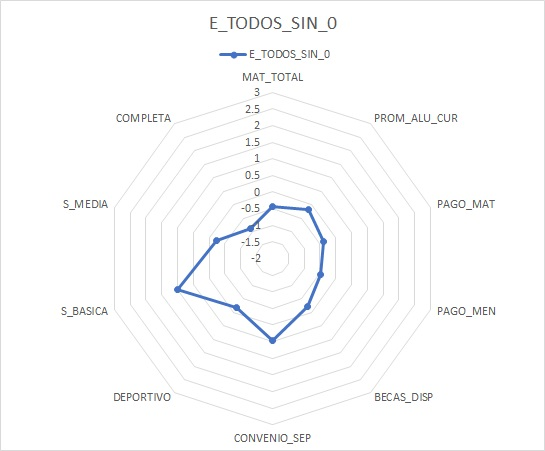
\includegraphics[width=7.3cm]{images/establecimientos/radar_sin_0.jpg}}
  \subfloat[Clúster de establecimientos E\_TODOS\_SIN\_1.]{
   \label{f:radar_estab_sin_1}
    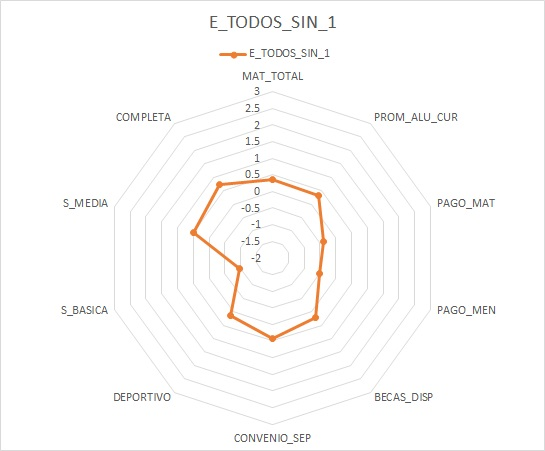
\includegraphics[width=7.3cm]{images/establecimientos/radar_sin_1.jpg}}\hspace{1mm}
  \subfloat[Clúster de establecimientos E\_TODOS\_SIN\_2.]{
   \label{f:radar_estab_sin_2}
    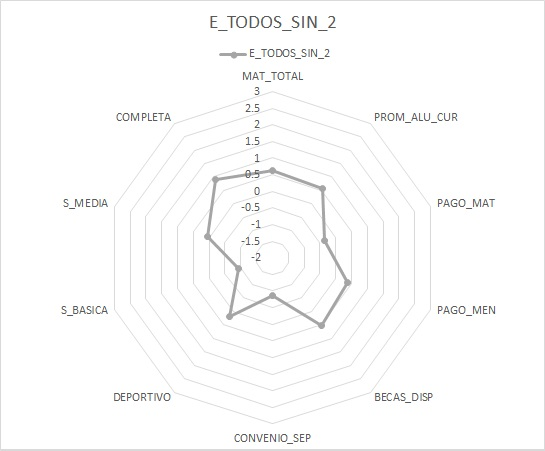
\includegraphics[width=7.3cm]{images/establecimientos/radar_sin_2.jpg}}
  \subfloat[Clúster de establecimientos E\_TODOS\_SIN\_3.]{
   \label{f:radar_estab_sin_3}
    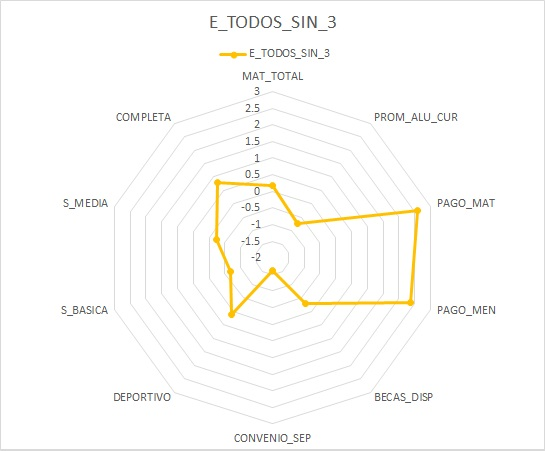
\includegraphics[width=7.3cm]{images/establecimientos/radar_sin_3.jpg}}
 \caption{Promedios de atributos normalizados de establecimientos de la Región Metropolitana.}
 \label{f:radar_estab_sin}
\end{figure}

\begin{table}[H]
\centering
\caption{Clústers de matrículas.}
\label{tab:cl_dependencia_sin}
\begin{tabular}{|c|c|c|c|c|}
\hline
\textbf{Clúster} & \textbf{Municipal} & \textbf{P. Subvencionado} & \textbf{P. Pagado} & \textbf{Corp. Admin. Del.}   \\ \hline
E\_TODOS\_SIN\_0 & 485 & 491 & 1 & 0 \\ \hline
E\_TODOS\_SIN\_1 & 173 & 318 & 0 & 33 \\ \hline
E\_TODOS\_SIN\_2 & 3 & 303 & 2 & 0 \\ \hline
E\_TODOS\_SIN\_3 & 0 & 1 & 258 & 0 \\ \hline
\end{tabular}
\end{table}

De la misma forma se caracterizan los clústers generados al incorporar las variables de relación establecimiento - matrículas, lo que se observa en la figura \ref{f:radar_estab_con} y la tabla \ref{tab:cl_dependencia_con}.

\begin{itemize}
    \item E\_TODOS\_CON\_0: Colegios particulares subvencionados y municipales principalmente de educación básica de matrícula gratuita y mensualidad gratuita o de precio bajo (menor a \$25.000). Poseen convenio SEP e IDE entre 0,5 y 1. Promedio de matrículas: 383, de alumnos por curso: 26 y de becas: 19. La distancia que deben recorrer sus alumnos es de 2.960 (percentil 75). El promedio de sobre edad es de 0,524 y 31\% son mayor o igual a 1 año. Estos se distribuyen de la siguiente forma según los años de sobre edad: 74,8\% (1), 18,9\% (2), 5,2\% (3) y 1,1\% (4).
    \item E\_TODOS\_CON\_1: Colegios principalmente particulares subvencionados, municipales y todos los de corporación de administración delegada con educación media o completa, de matrículas y mensualidades gratuitas o de precio bajo (menor a \$25.000). Poseen convenio SEP e IDE entre -0,5 y 0. Promedio de matrículas: 781, de alumnos por curso: 30 y de becas: 58. La distancia que deben recorrer sus alumnos es de 5.204 (percentil 75). El promedio de sobre edad es de 0,488 y 32,9\% son mayor o igual a 1 año. Estos se distribuyen de la siguiente forma según los años de sobre edad: 75,1\% (1), 20,6\% (2), 3,9\% (3) y 0,5\% (4).
    \item E\_TODOS\_CON\_2: Colegios particulares subvencionados de educación media o completa con matrículas bajas (menor a \$10.000) y mensualidades medias (\$25.000 - \$100.000). En su mayoría no poseen convenio SEP, nivel deportivo bajo e IDE entre 0 y 1,5. Promedio de matrículas: 895, de alumnos por curso: 32 y de becas: 91. La distancia que deben recorrer sus alumnos es de 5.207 (percentil 75). El promedio de sobre edad es de 0,297 y 24\% son mayor o igual a 1 año. Estos se distribuyen de la siguiente forma según los años de sobre edad: 85,3\% (1), 13\% (2), 1,6\% (3) y 0,1\% (4).
    \item E\_TODOS\_CON\_3: Colegios particulares pagados principalmente de educación completa con matrículas y mensualidades elevadas (sobre \$50.000). No poseen convenio SEP y su IDE esta 0,5, pero predominantemente entre 1 y 1,5. Promedio de matrículas: 686, de alumnos por curso: 21 y de becas: 8. La distancia que deben recorrer sus alumnos es de 9.761 (percentil 75). El promedio de sobre edad es de 0,488 y 38,1\% son mayor o igual a 1 año. Estos se distribuyen de la siguiente forma según los años de sobre edad: 94,9\% (1), 4,6\% (2), 0,4\% (3) y 0\% (4).
\end{itemize}

\begin{figure}[H]
 \centering
  \subfloat[Clúster de establecimientos E\_TODOS\_CON\_0.]{
   \label{f:radar_estab_con_0}
    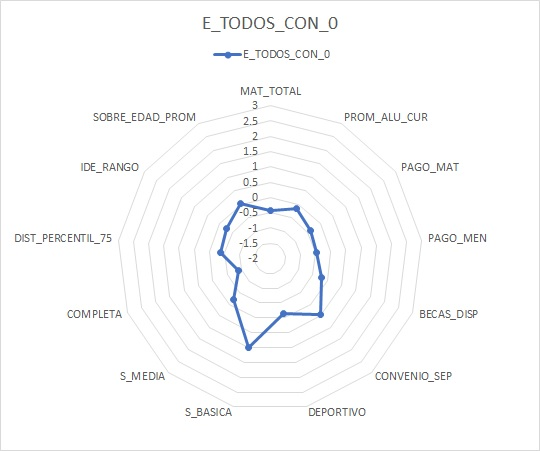
\includegraphics[width=7.3cm]{images/establecimientos/radar_con_0.jpg}}
  \subfloat[Clúster de establecimientos E\_TODOS\_CON\_1.]{
   \label{f:radar_estab_con_1}
    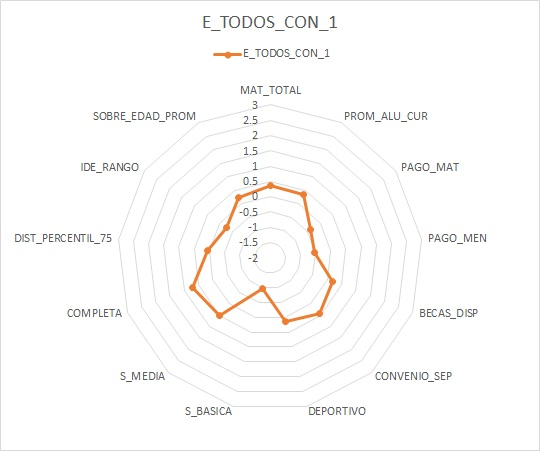
\includegraphics[width=7.3cm]{images/establecimientos/radar_con_1.jpg}}\hspace{1mm}
  \subfloat[Clúster de establecimientos E\_TODOS\_CON\_2.]{
   \label{f:radar_estab_con_2}
    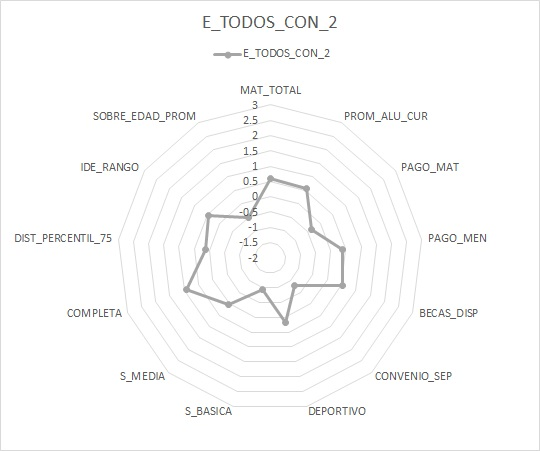
\includegraphics[width=7.3cm]{images/establecimientos/radar_con_2.jpg}}
  \subfloat[Clúster de establecimientos E\_TODOS\_CON\_3.]{
   \label{f:radar_estab_con_3}
    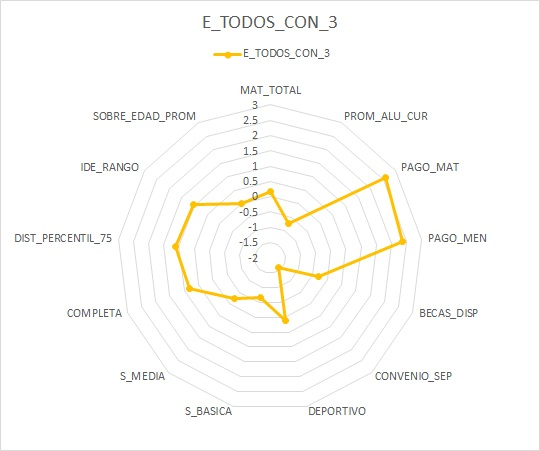
\includegraphics[width=7.3cm]{images/establecimientos/radar_con_3.jpg}}
 \caption{Promedios de atributos normalizados de establecimientos (con atributos relacionales) de la Región Metropolitana.}\
 \label{f:radar_estab_con}
\end{figure}

\begin{table}[H]
\centering
\caption{Clústers de matrículas.}
\label{tab:cl_dependencia_con}
\begin{tabular}{|c|c|c|c|c|}
\hline
\textbf{Clúster} & \textbf{Municipal} & \textbf{P. Subvencionado} & \textbf{P. Pagado} & \textbf{Corp. Admin. Del.}   \\ \hline
E\_TODOS\_CON\_0 & 485 & 489 & 1 & 0 \\ \hline
E\_TODOS\_CON\_1 & 173 & 307 & 0 & 33 \\ \hline
E\_TODOS\_CON\_2 & 3 & 316 & 2 & 0 \\ \hline
E\_TODOS\_CON\_3 & 0 & 1 & 258 & 0 \\ \hline
\end{tabular}
\end{table}

Al momento de comparar ambos resultados se puede ver que al incluir las variables de relación los clústers no muestran una gran variación, pero si aumenta el nivel de detalle de cada clúster. A partir de esto se aprecia que los primeros dos clústers son colegios gratuitos o baratos con un IDE bajo que se diferencian entre ellos principalmente por el nivel de educación que imparten. El tercer clúster se diferencia de los anteriores en que su nivel de copago es de un nivel medio al igual que su IDE. Finalmente el cuarto clúster tiene un nivel de copago elevado y un mejor IDE. Un factor que los diferencia a todos es la distancia que recorren sus estudiantes para llegar al establecimiento, ya que desde el primero al cuarto la distancia va en aumento. Finalmente otro punto interesante de analizar es la sobre edad, que en el caso de los colegios mas caros se concentra con un 95\% en un año de sobre edad. En el resto de los clústers el valor fluctúa entre un 75\% y 85\%, y el resto de distribuye de 2 a 4 años de sobre edad.

\begin{figure}[H]
 \centering
  \subfloat[Clúster de matrículas M\_TODAS\_SIN\_0.]{
   \label{f:radar_estab_con_0}
    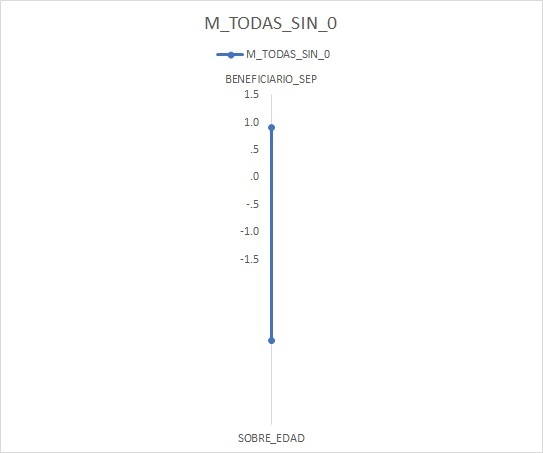
\includegraphics[width=7.3cm]{images/matriculas/radar_mat_sin_0.jpg}}
  \subfloat[Clúster de matrículas M\_TODAS\_SIN\_1.]{
   \label{f:radar_estab_con_1}
    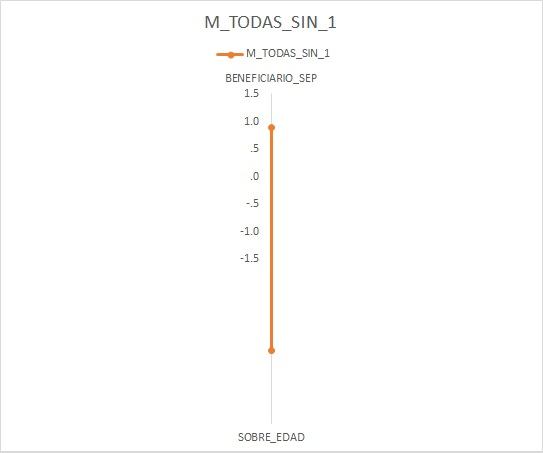
\includegraphics[width=7.3cm]{images/matriculas/radar_mat_sin_1.jpg}}\hspace{1mm}
  \subfloat[Clúster de matrículas M\_TODAS\_SIN\_2.]{
   \label{f:radar_estab_con_2}
    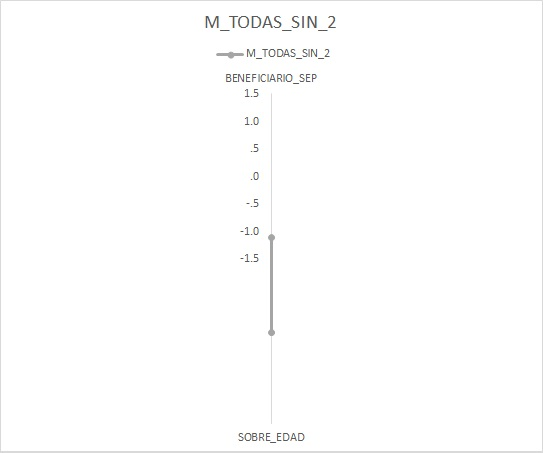
\includegraphics[width=7.3cm]{images/matriculas/radar_mat_sin_2.jpg}}
  \subfloat[Clúster de matrículas M\_TODAS\_SIN\_3.]{
   \label{f:radar_estab_con_3}
    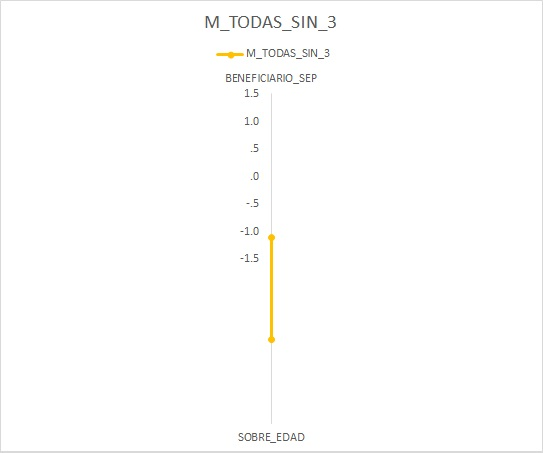
\includegraphics[width=7.3cm]{images/matriculas/radar_mat_sin_3.jpg}}
 \caption{Promedios de atributos normalizados de matrículas de la Región Metropolitana.}\
 \label{f:radar_estab_con}
\end{figure}

\begin{figure}[H]
 \centering
  \subfloat[Clúster de matrículas M\_TODAS\_CON\_0.]{
   \label{f:radar_estab_con_0}
    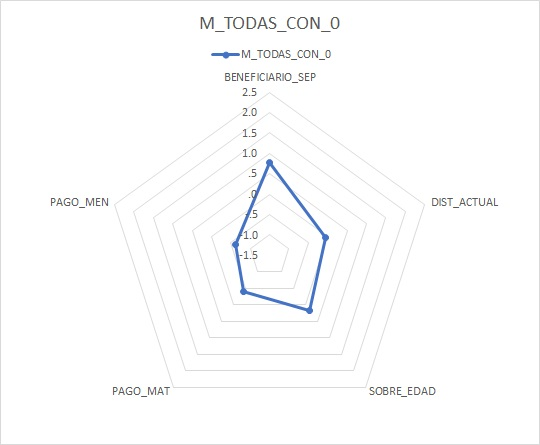
\includegraphics[width=7.3cm]{images/matriculas/radar_mat_con_0.jpg}}
  \subfloat[Clúster de matrículas M\_TODAS\_CON\_1.]{
   \label{f:radar_estab_con_1}
    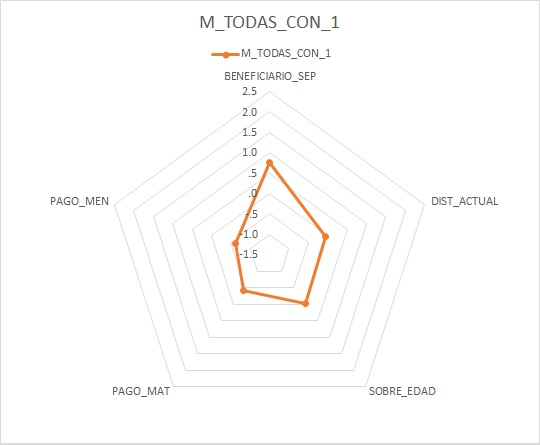
\includegraphics[width=7.3cm]{images/matriculas/radar_mat_con_1.jpg}}\hspace{1mm}
  \subfloat[Clúster de matrículas M\_TODAS\_CON\_2.]{
   \label{f:radar_estab_con_2}
    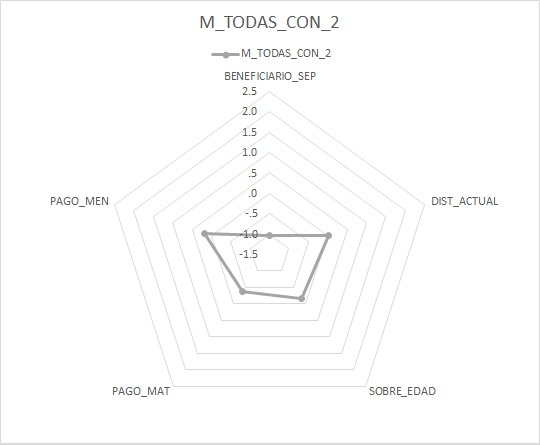
\includegraphics[width=7.3cm]{images/matriculas/radar_mat_con_2.jpg}}
  \subfloat[Clúster de matrículas M\_TODAS\_CON\_3.]{
   \label{f:radar_estab_con_3}
    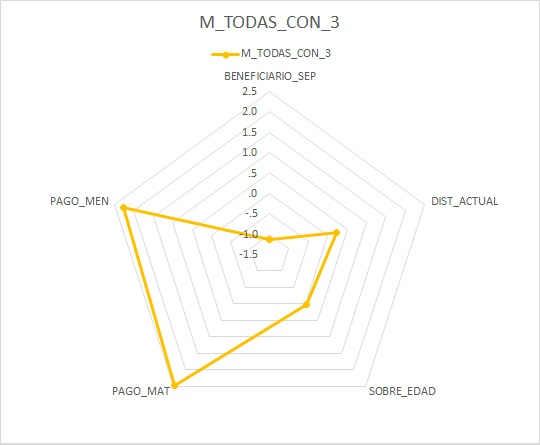
\includegraphics[width=7.3cm]{images/matriculas/radar_mat_con_3.jpg}}
 \caption{Promedios de atributos normalizados de matrículas (con atributos relacionales) de la Región Metropolitana.}\
 \label{f:radar_estab_con}
\end{figure}

\begin{figure}[H]
 \centering
  \subfloat[Establecimientos clúster E\_TODOS\_SIN\_0.]{
   \label{f:}
    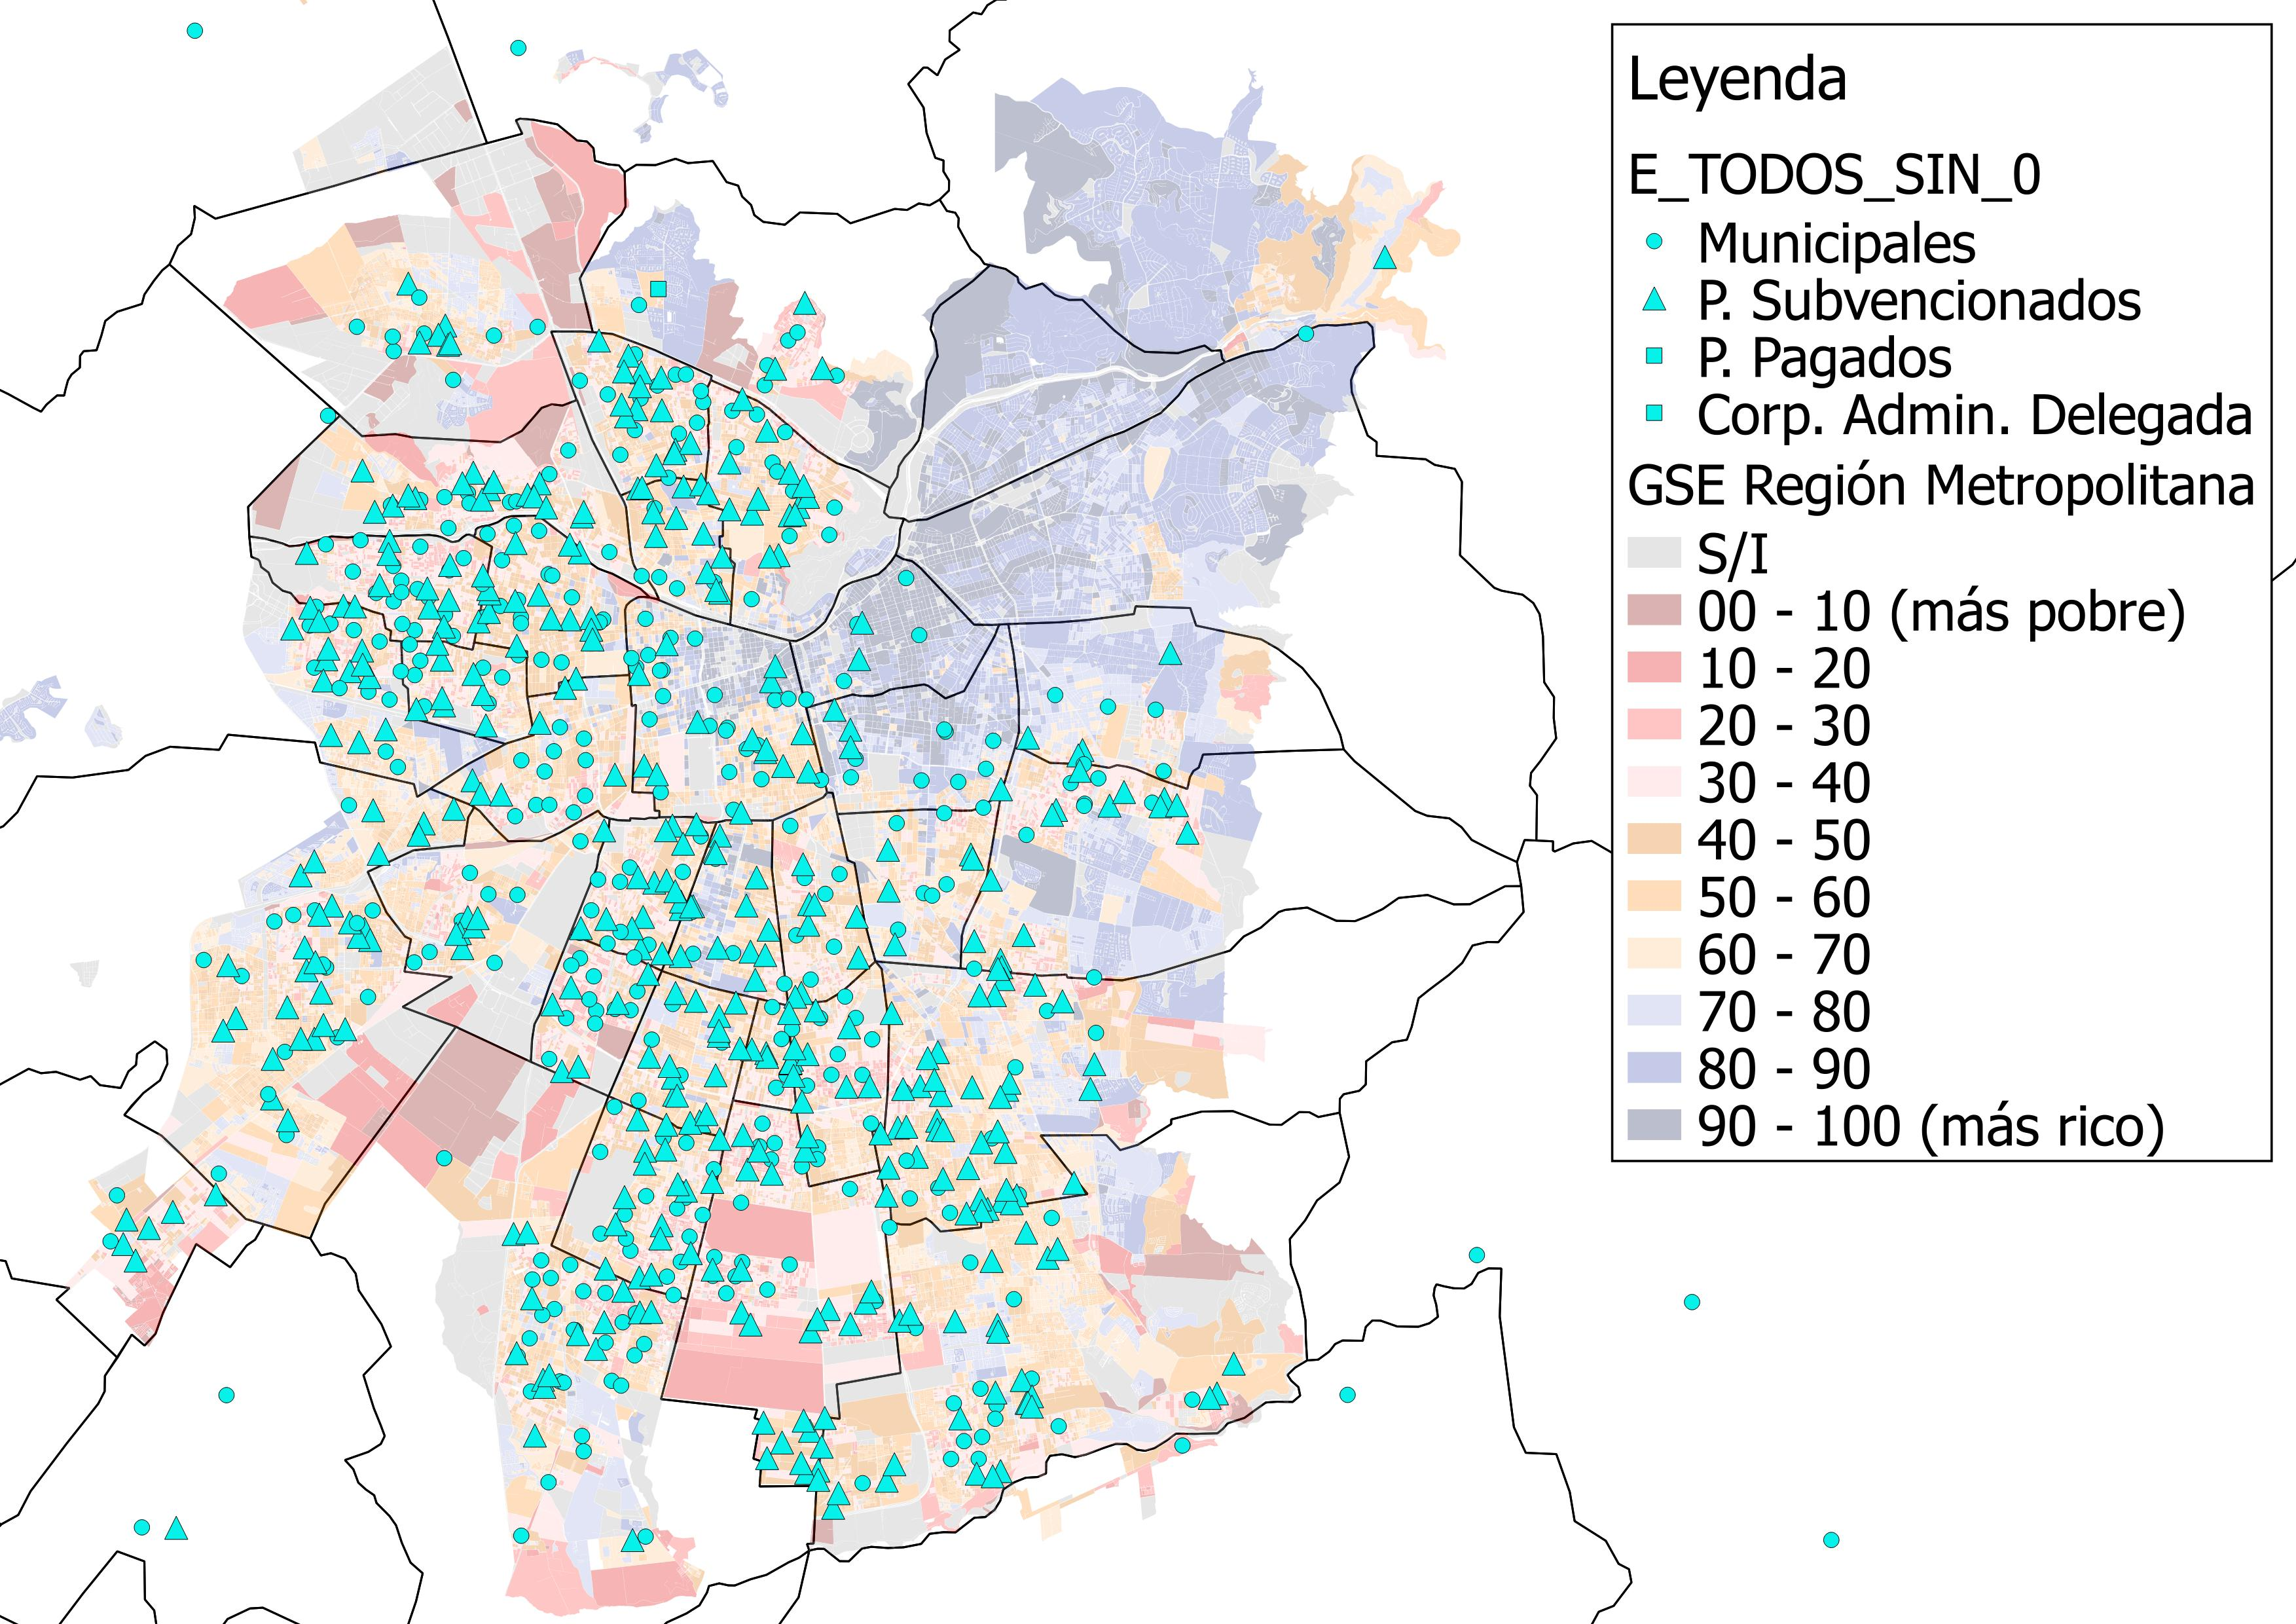
\includegraphics[width=7.5cm]{images/establecimientos/E_TODOS_SIN_0.jpg}}
  \subfloat[Establecimientos clúster E\_TODOS\_SIN\_1.]{
   \label{f:}
    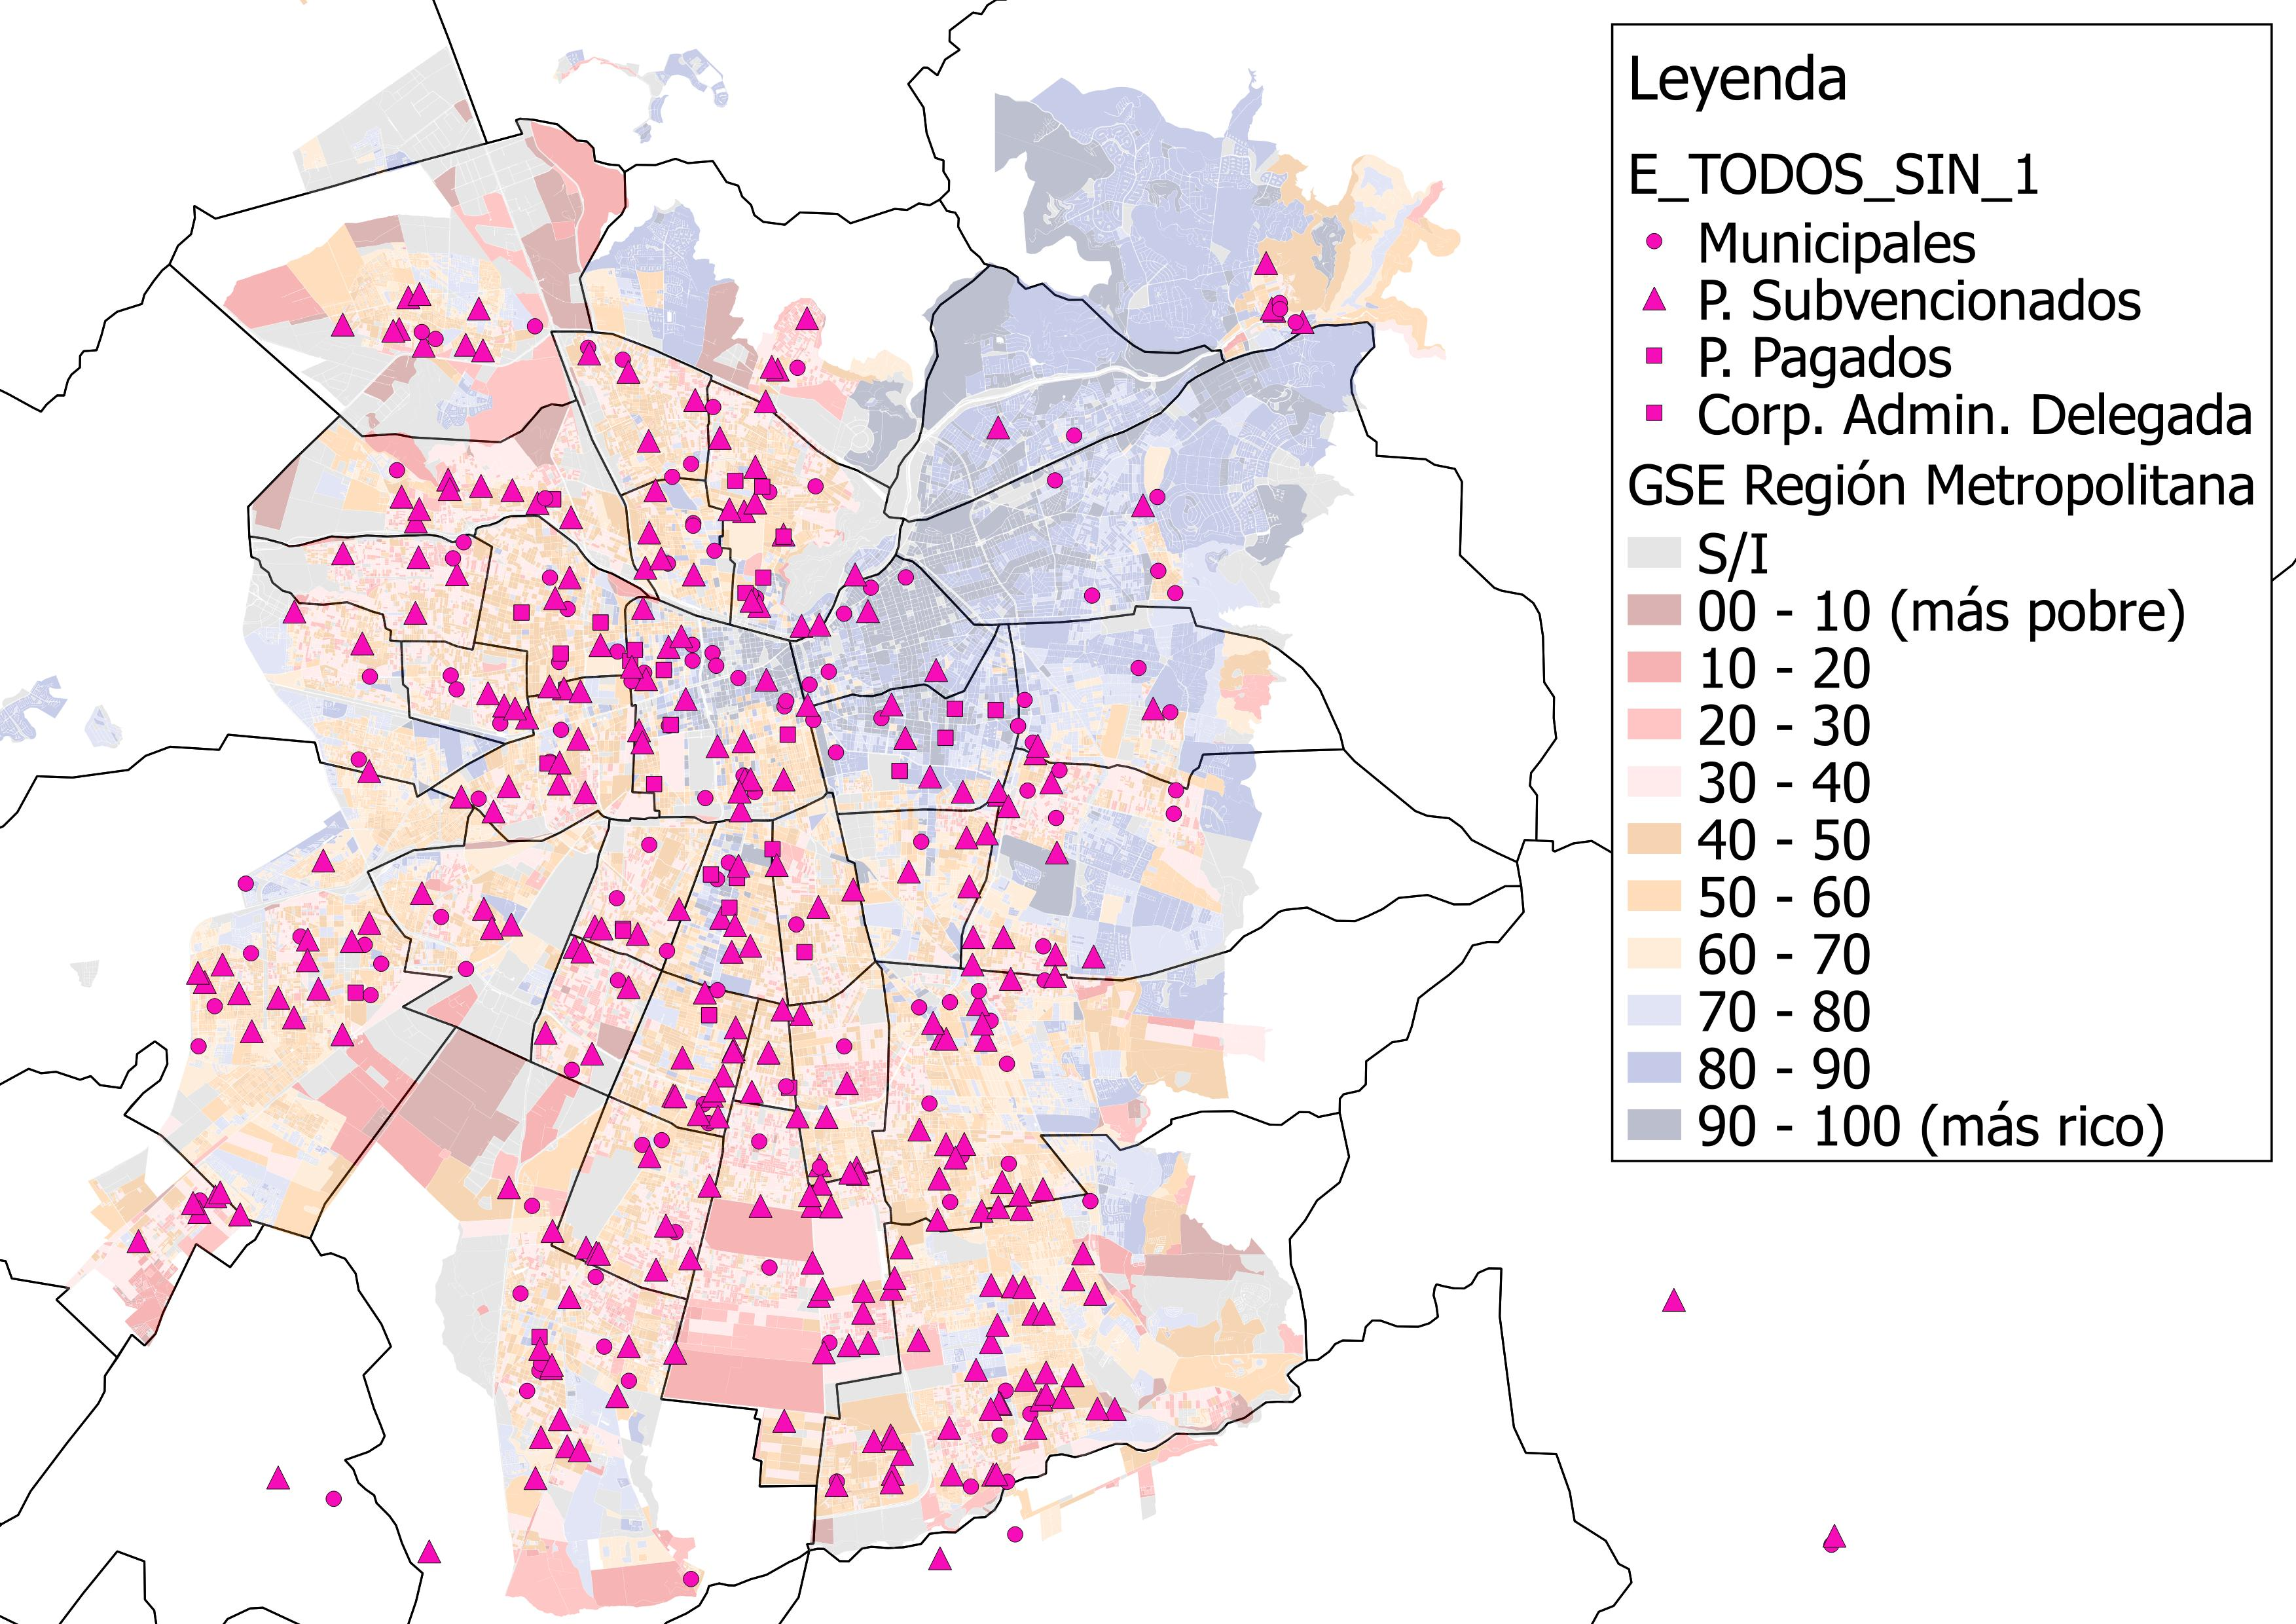
\includegraphics[width=7.5cm]{images/establecimientos/E_TODOS_SIN_1.jpg}}\hspace{1mm}
  \subfloat[Establecimientos clúster E\_TODOS\_SIN\_2.]{
   \label{f:}
    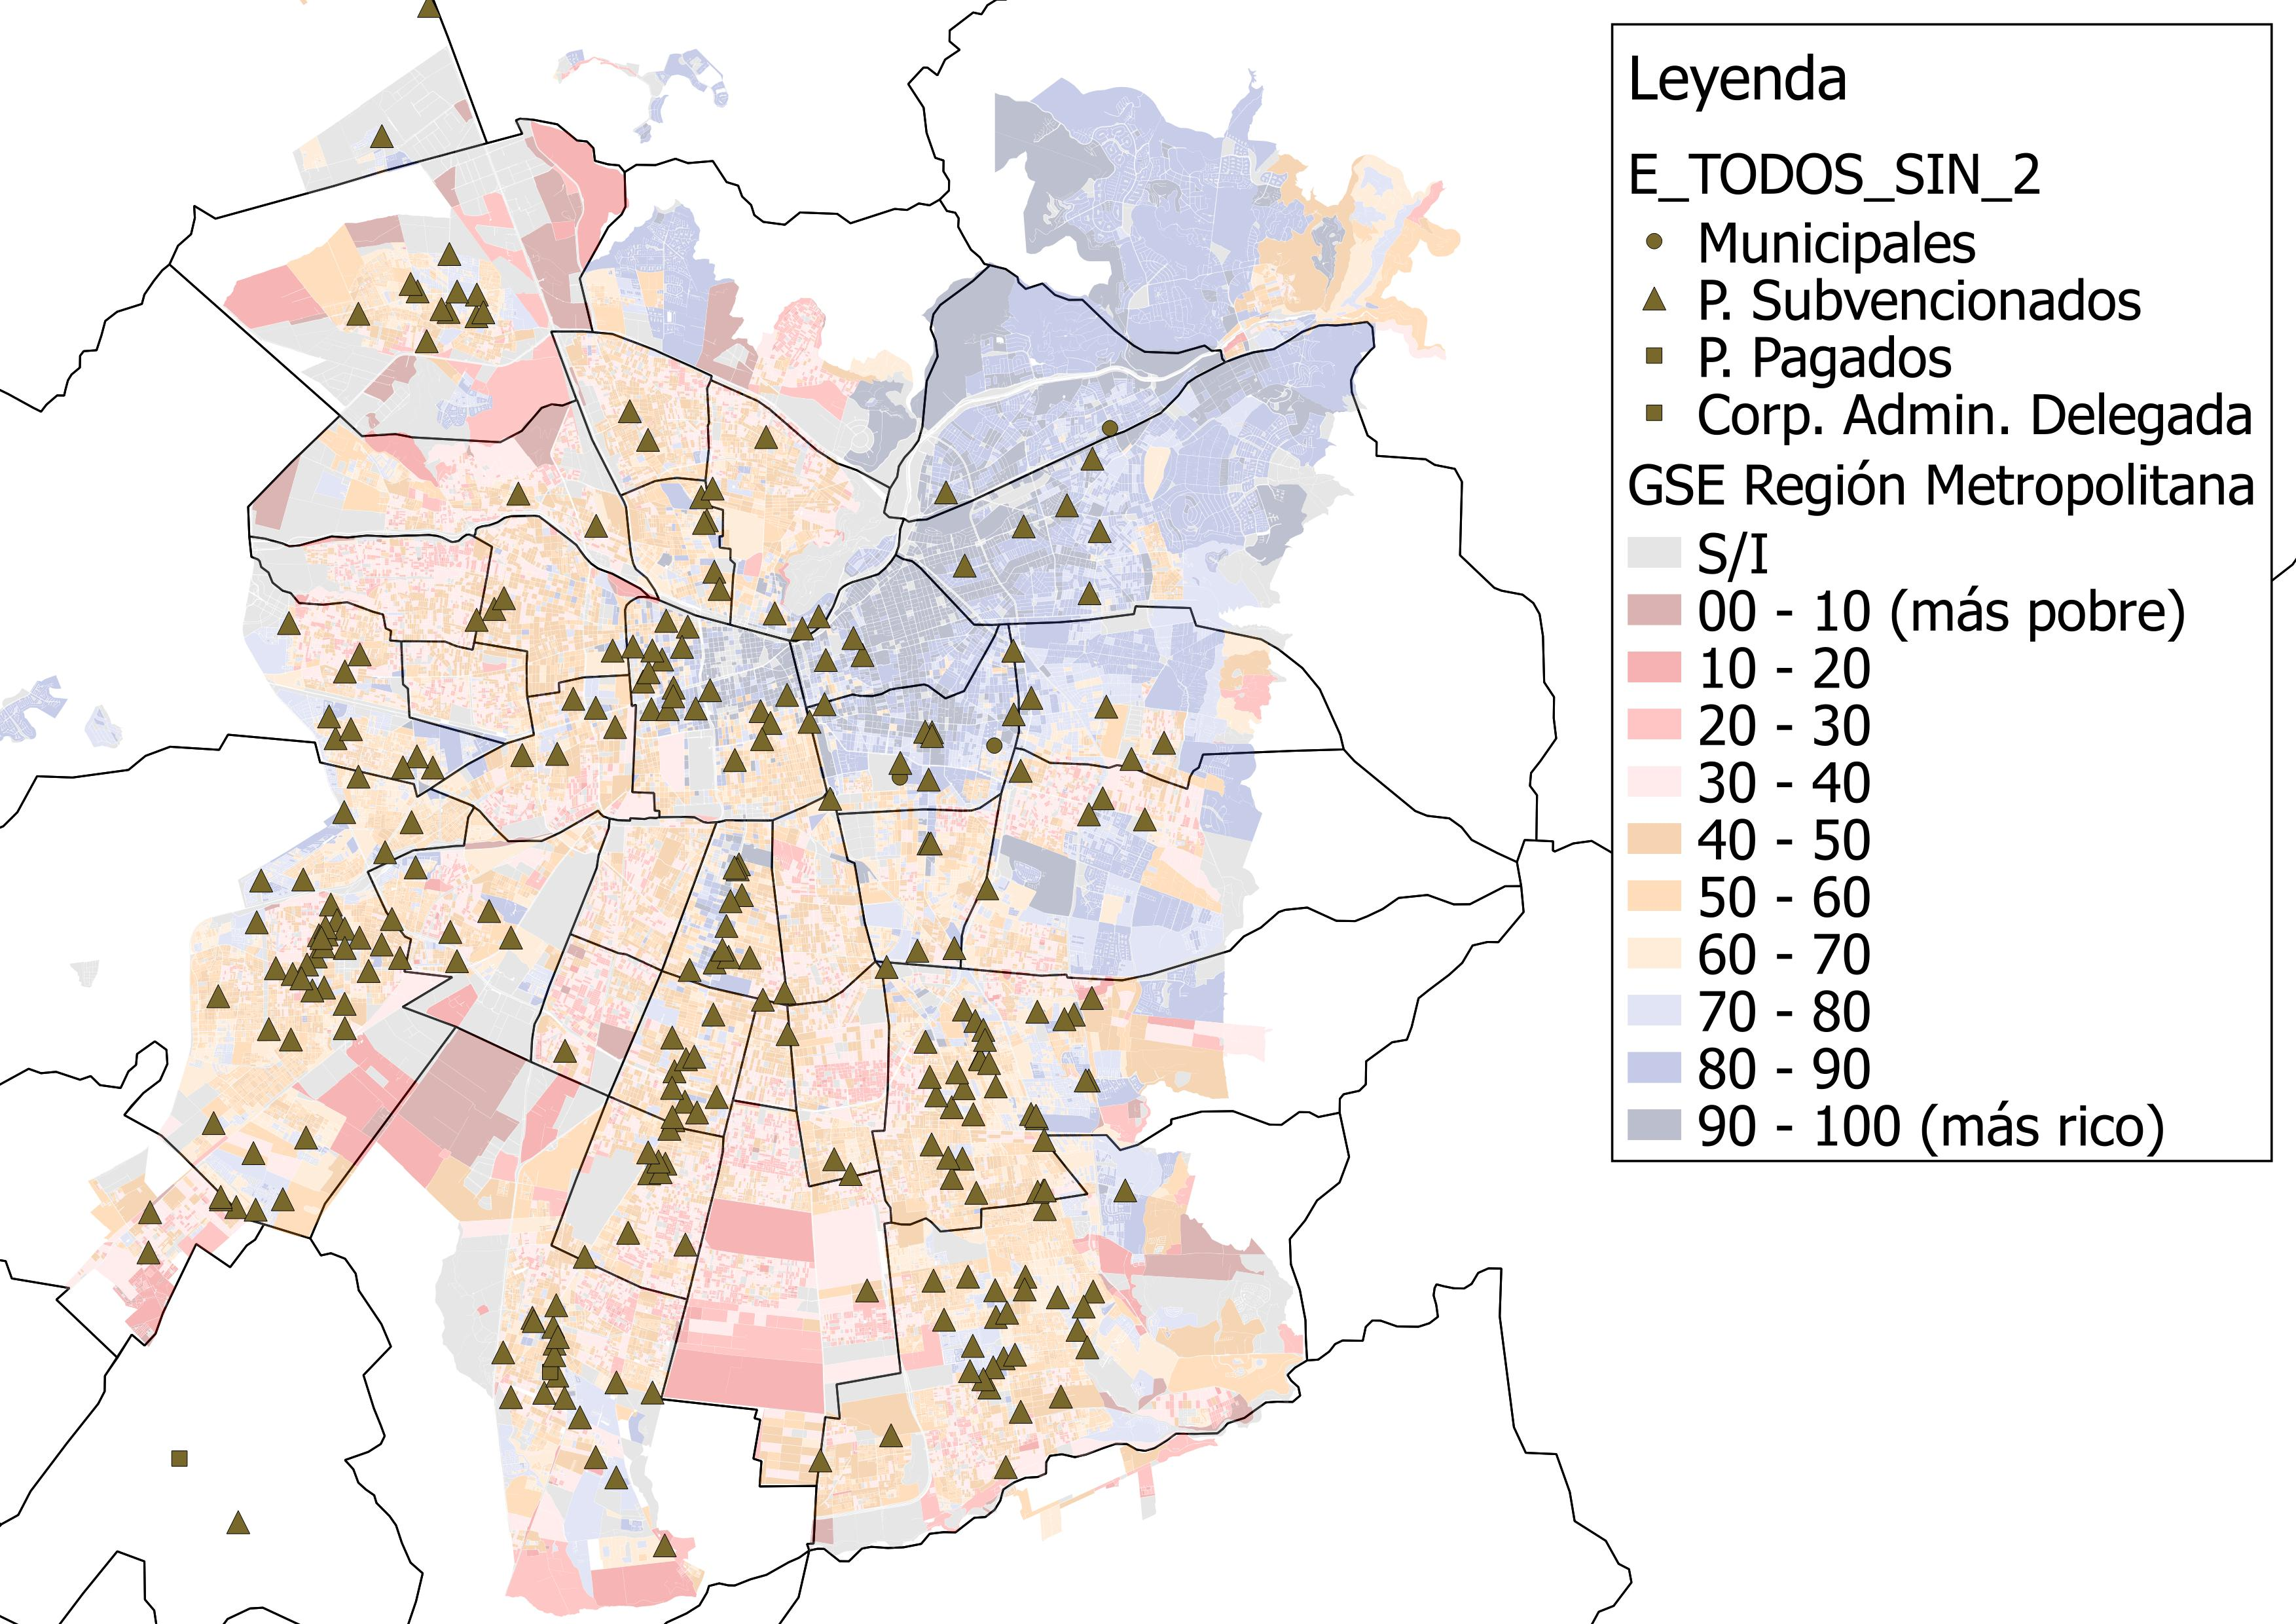
\includegraphics[width=7.5cm]{images/establecimientos/E_TODOS_SIN_2.jpg}}
  \subfloat[Establecimientos clúster E\_TODOS\_SIN\_3.]{
   \label{f:}
    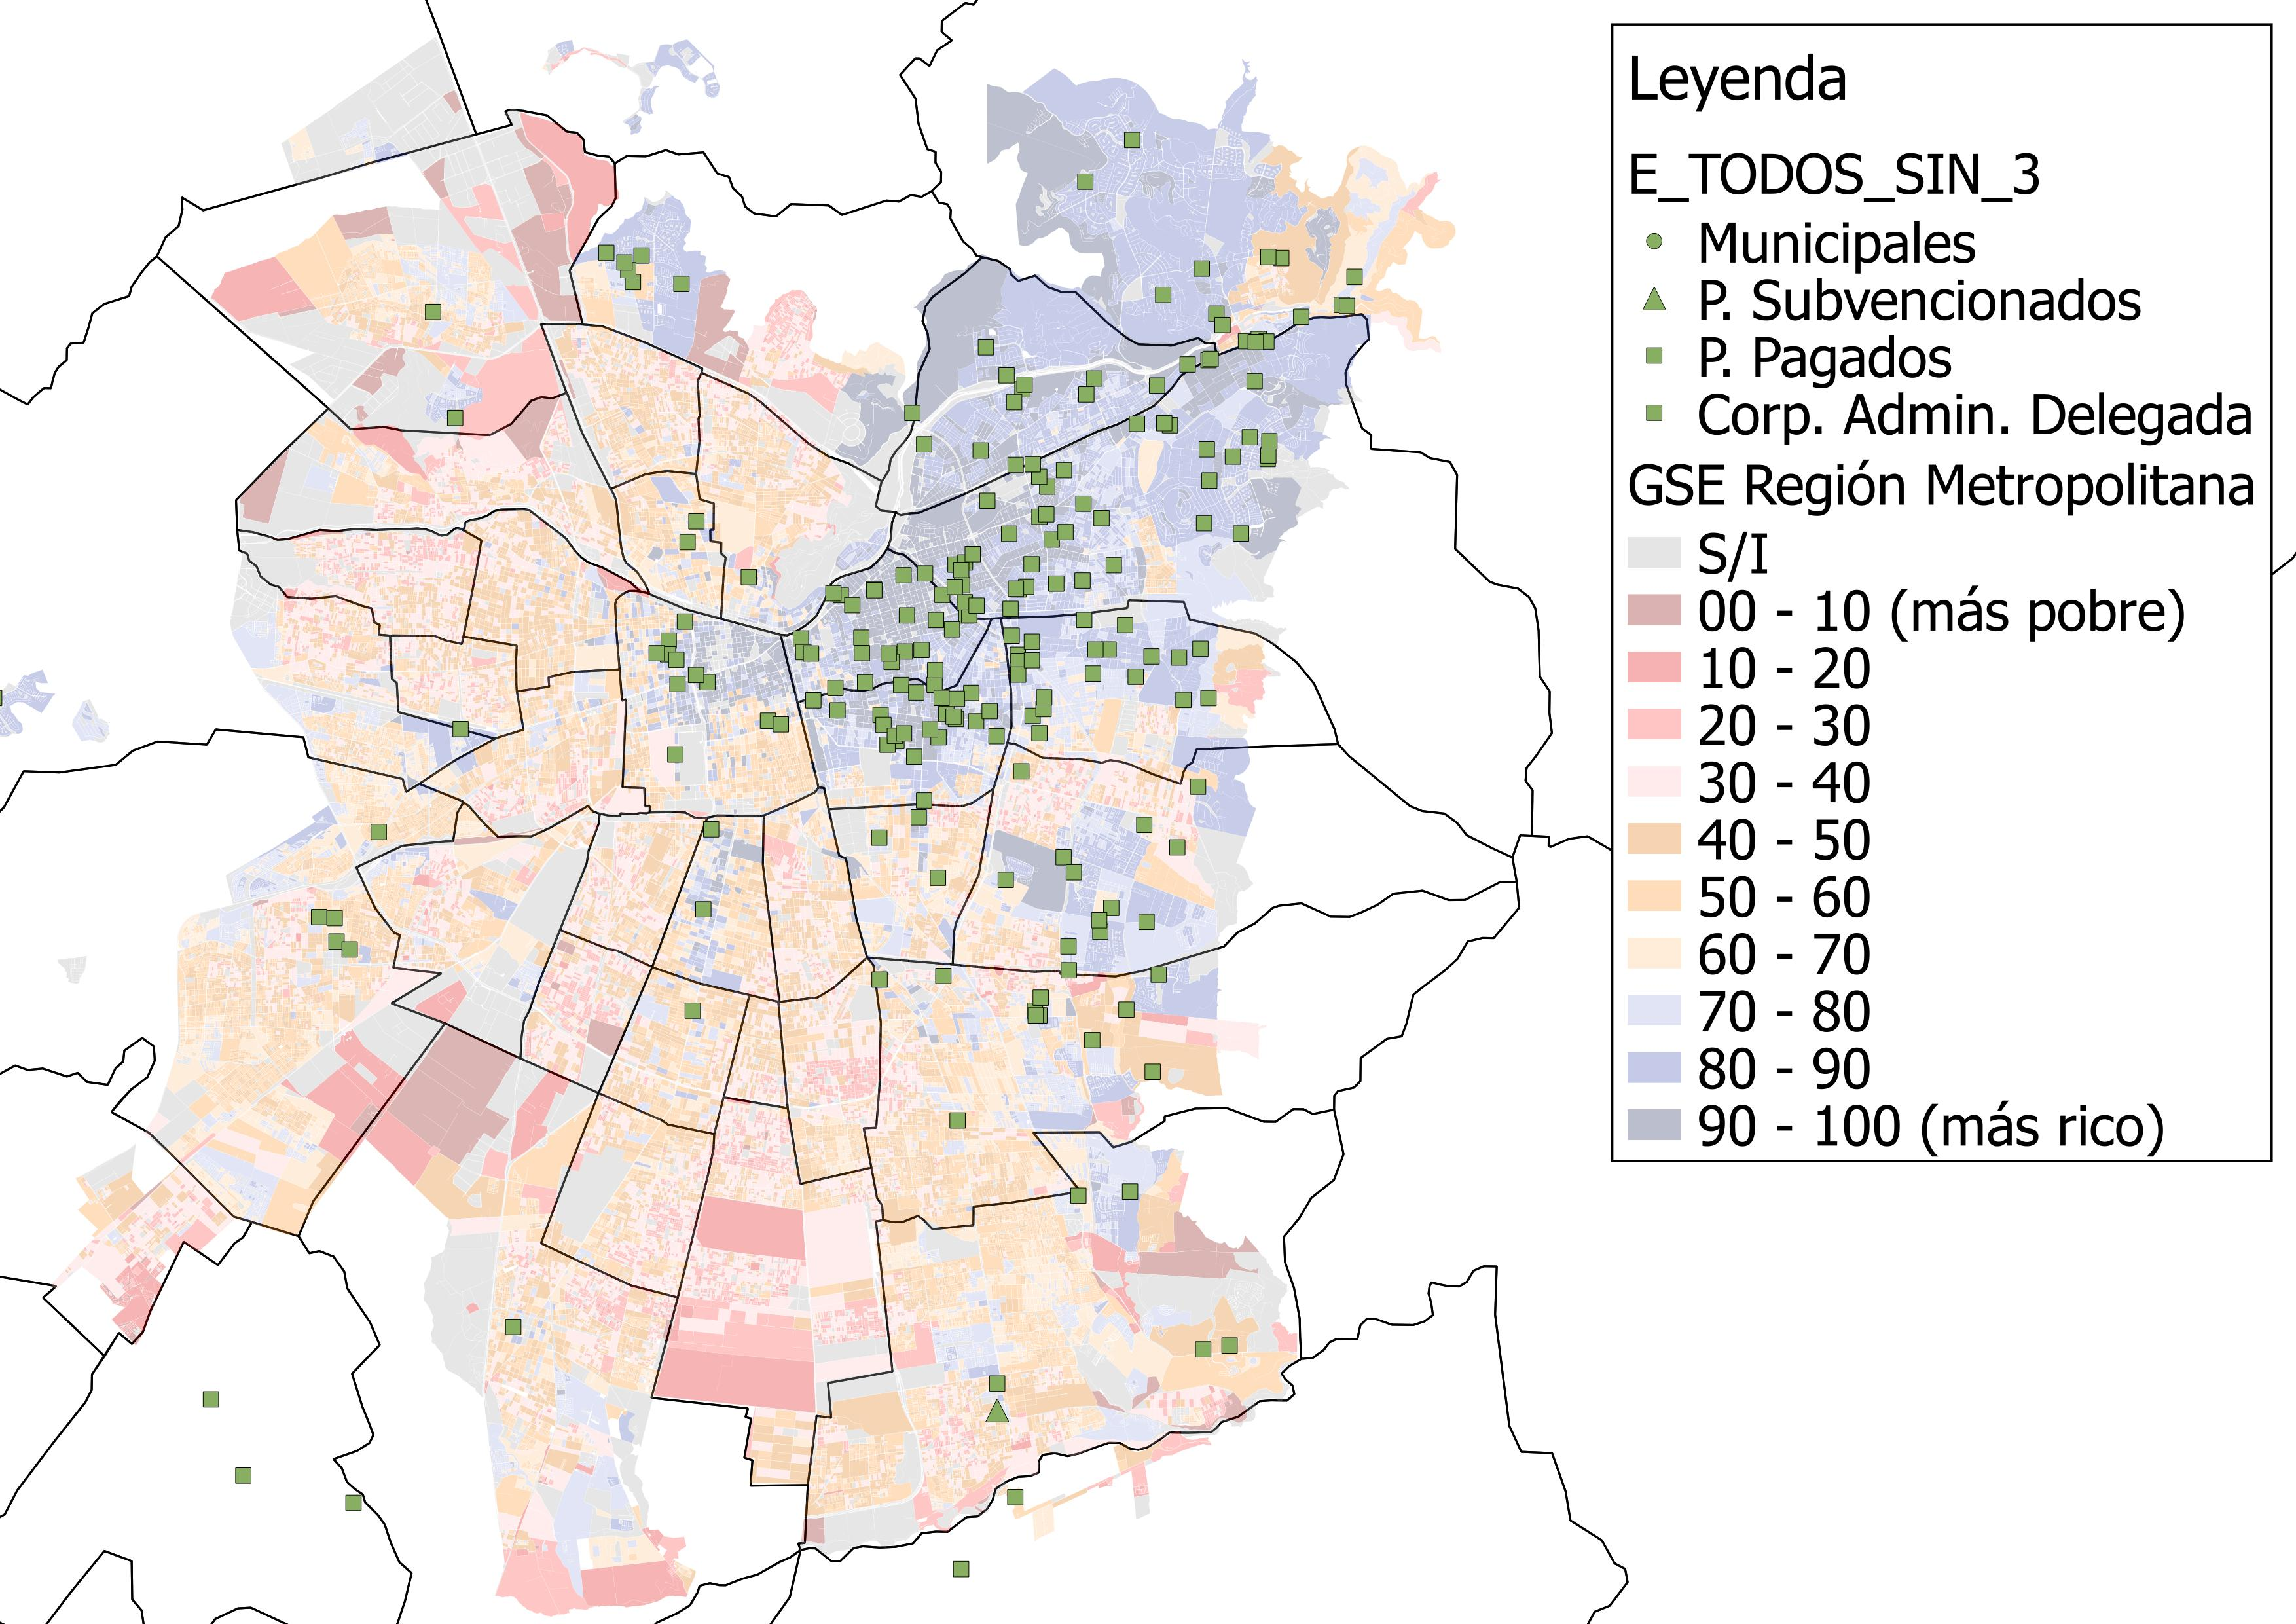
\includegraphics[width=7.5cm]{images/establecimientos/E_TODOS_SIN_3.jpg}}
 \caption{Mapas de clústers de establecimientos sobre mapa GSE de la Región Metropolitana.}
 \label{f:}
\end{figure}

\begin{figure}[H]
 \centering
  \subfloat[Establecimientos clúster E\_TODOS\_CON\_0.]{
   \label{f:}
    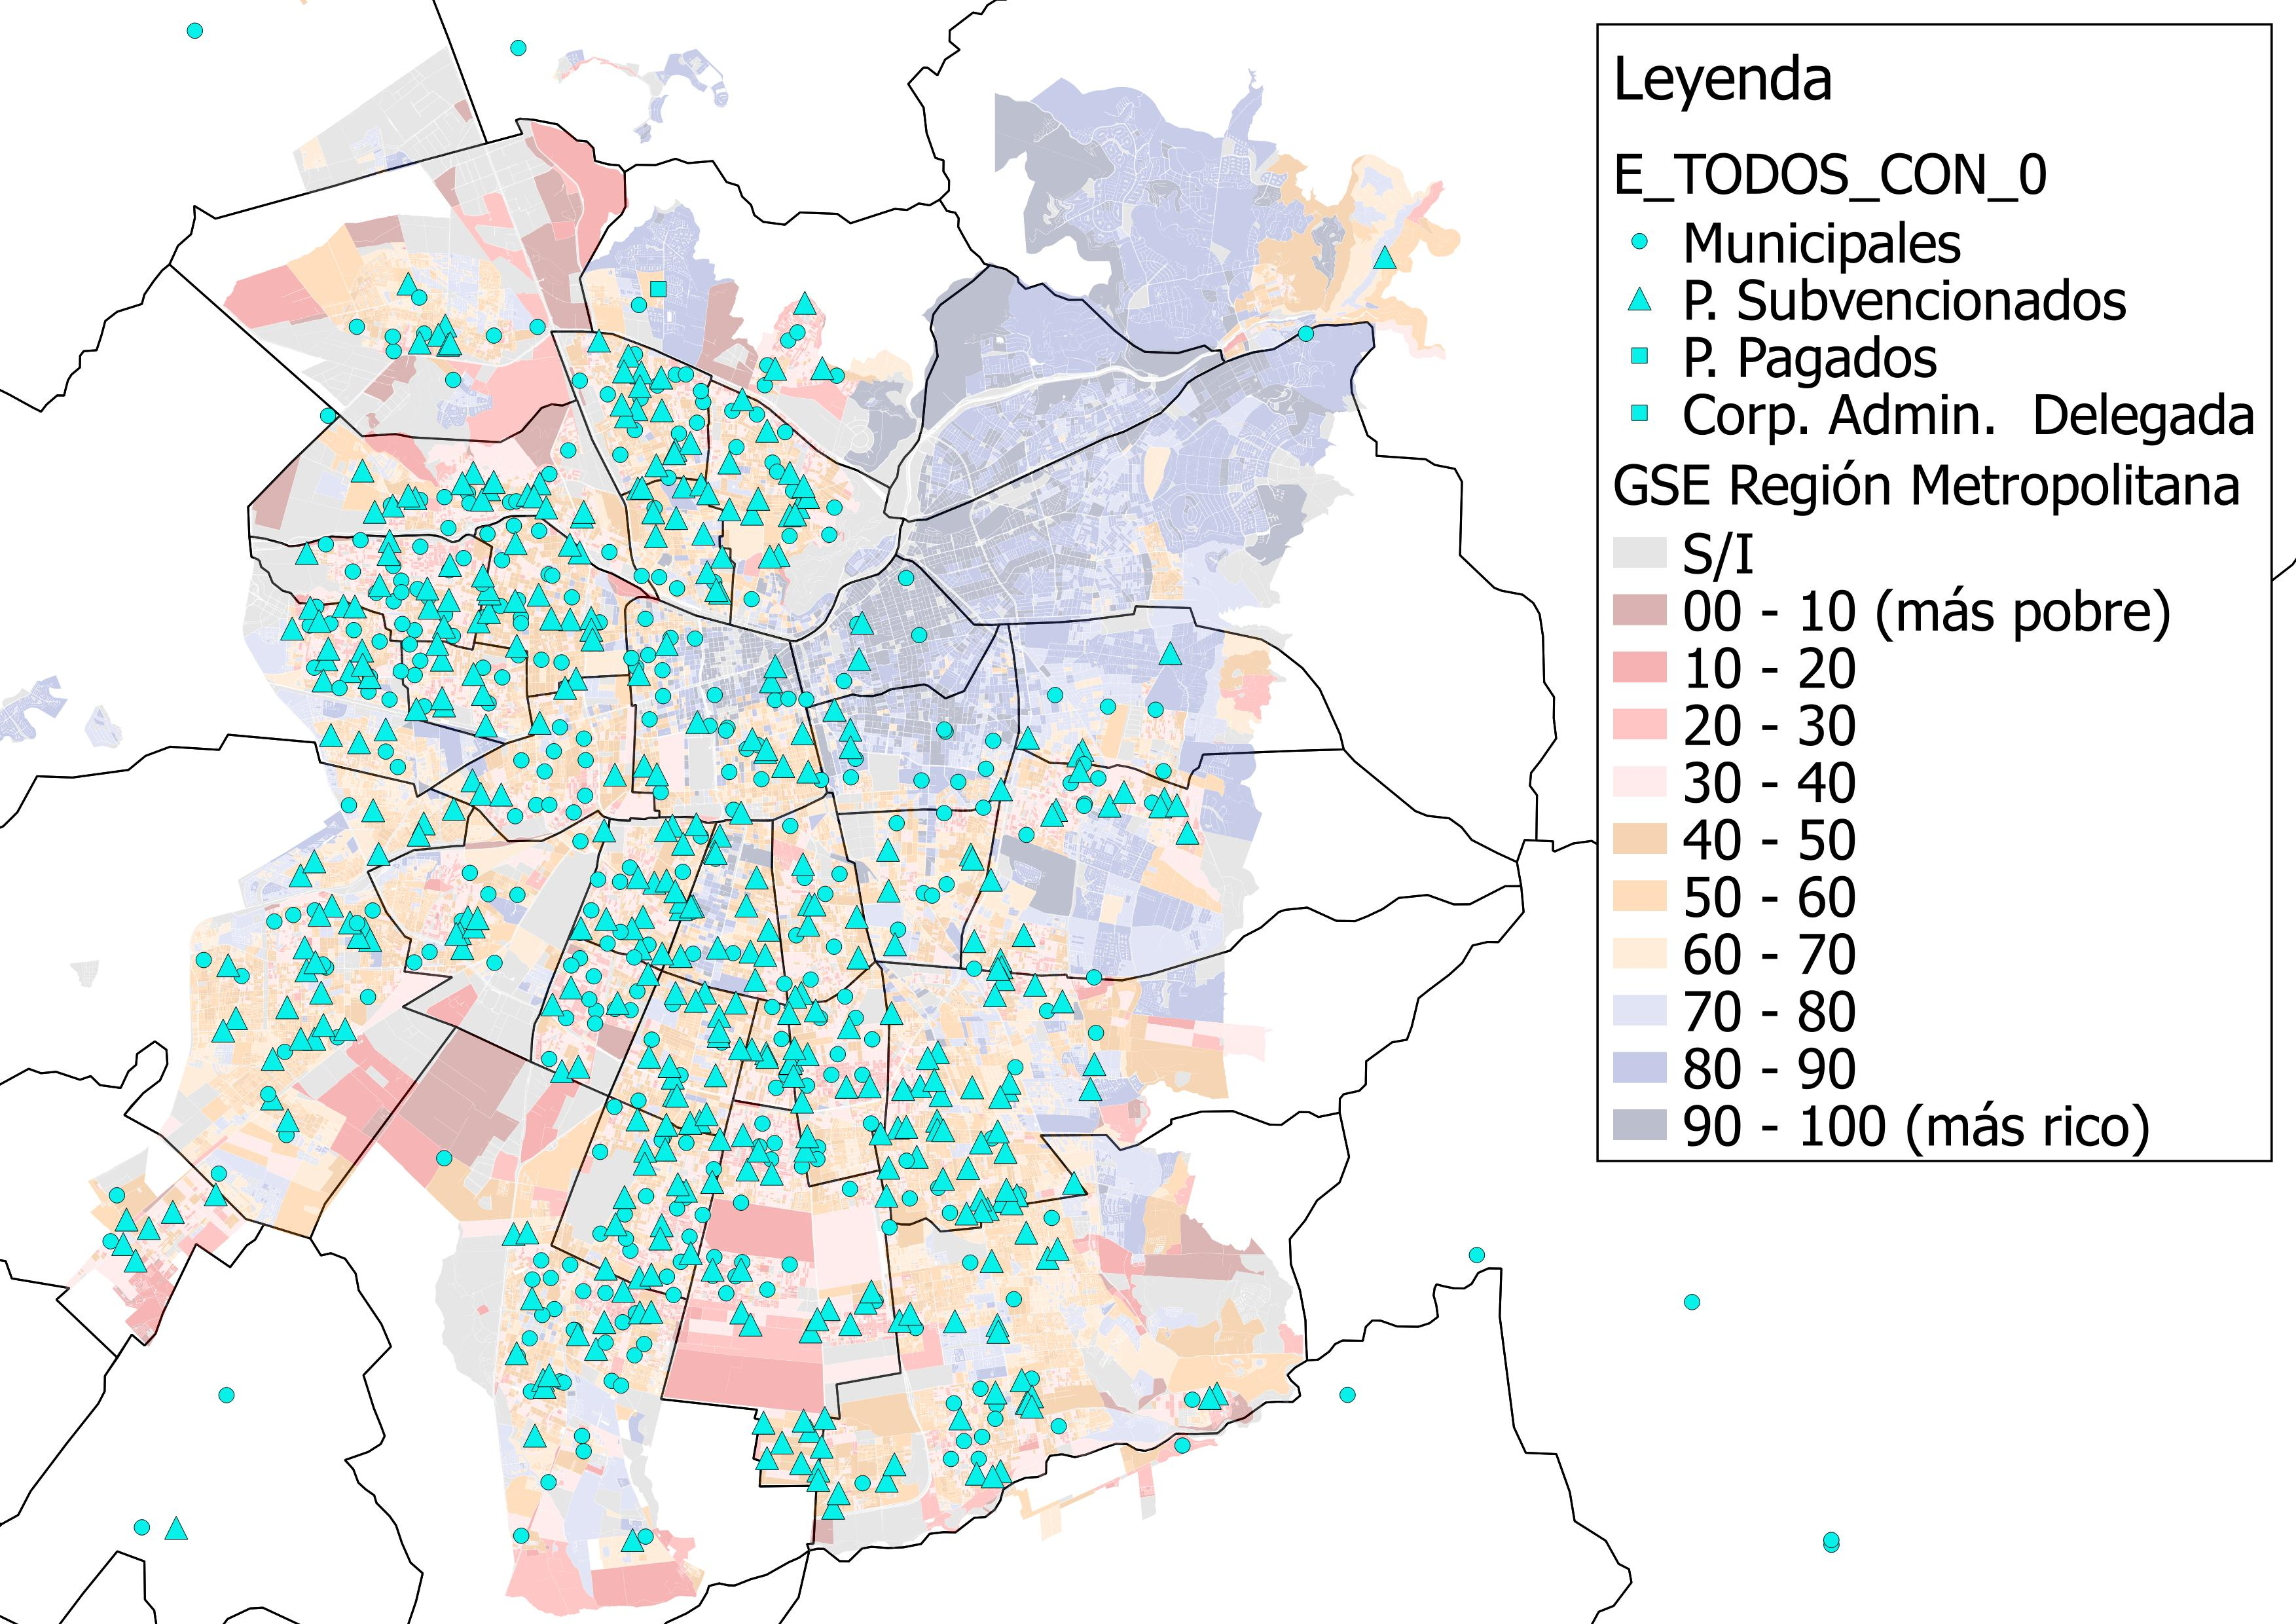
\includegraphics[width=7.5cm]{images/establecimientos/E_TODOS_CON_0.jpg}}
  \subfloat[Establecimientos clúster E\_TODOS\_CON\_1.]{
   \label{f:}
    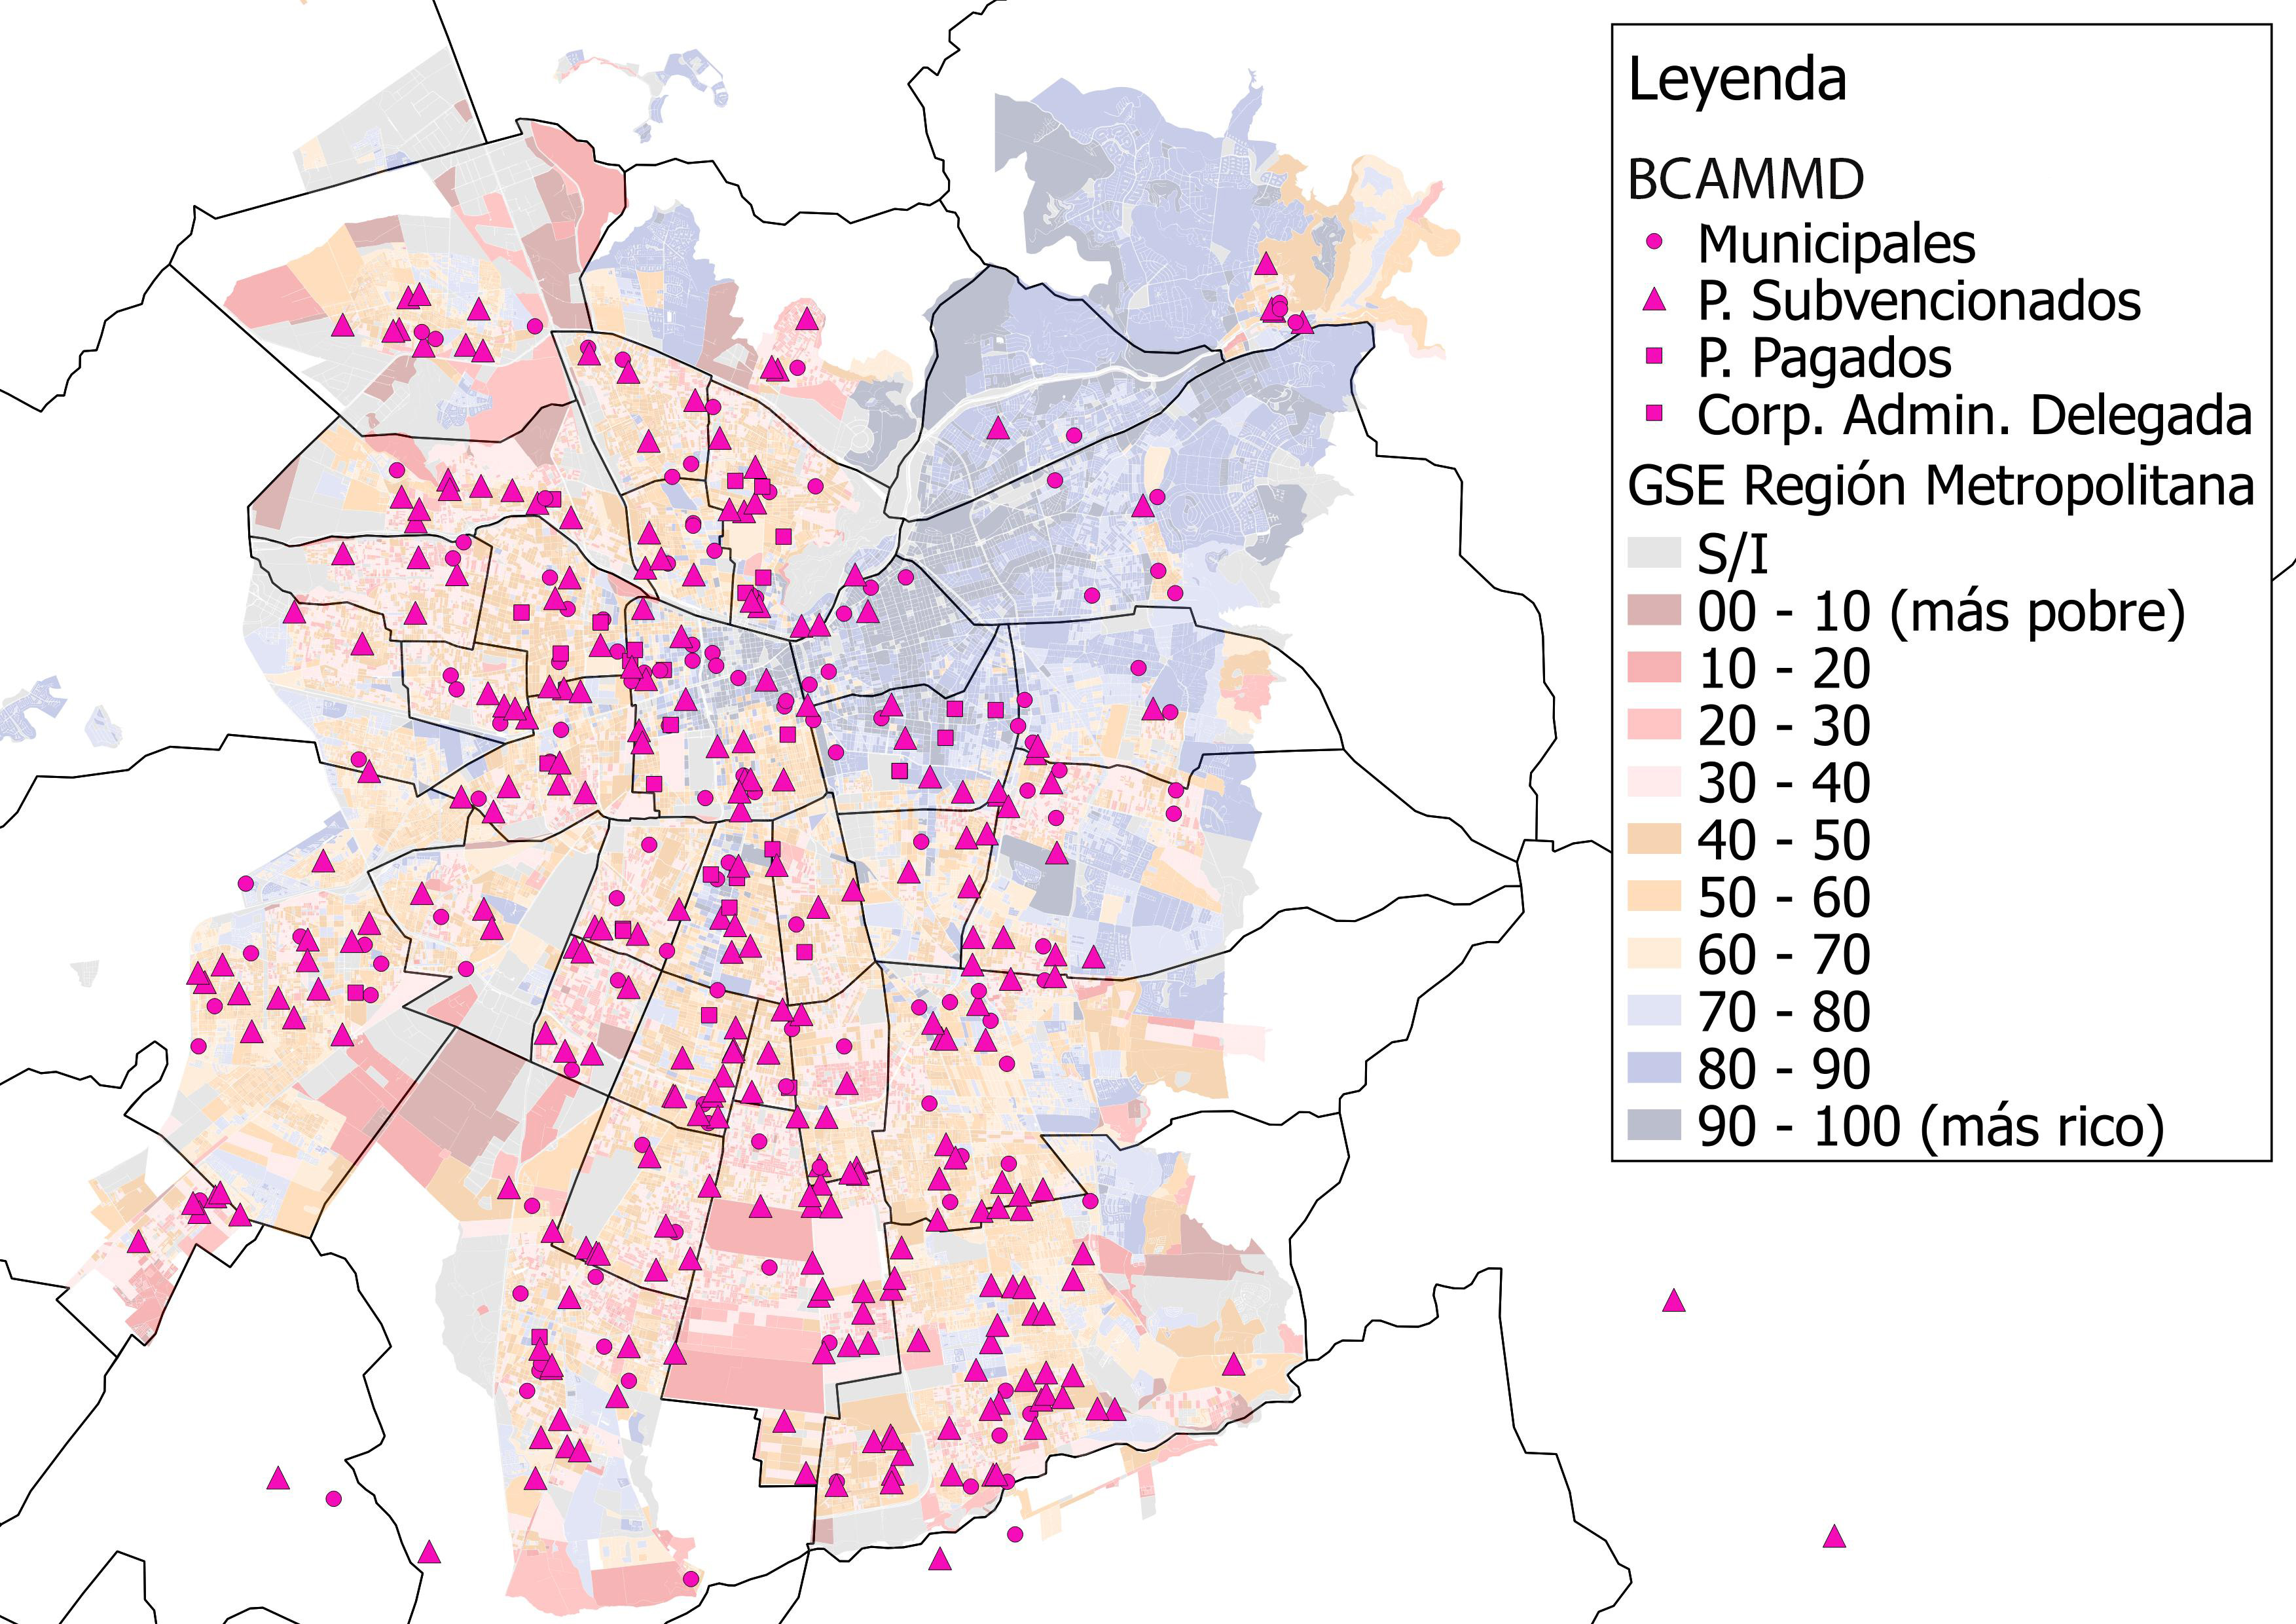
\includegraphics[width=7.5cm]{images/establecimientos/E_TODOS_CON_1.jpg}}\hspace{1mm}
  \subfloat[Establecimientos clúster E\_TODOS\_CON\_2.]{
   \label{f:}
    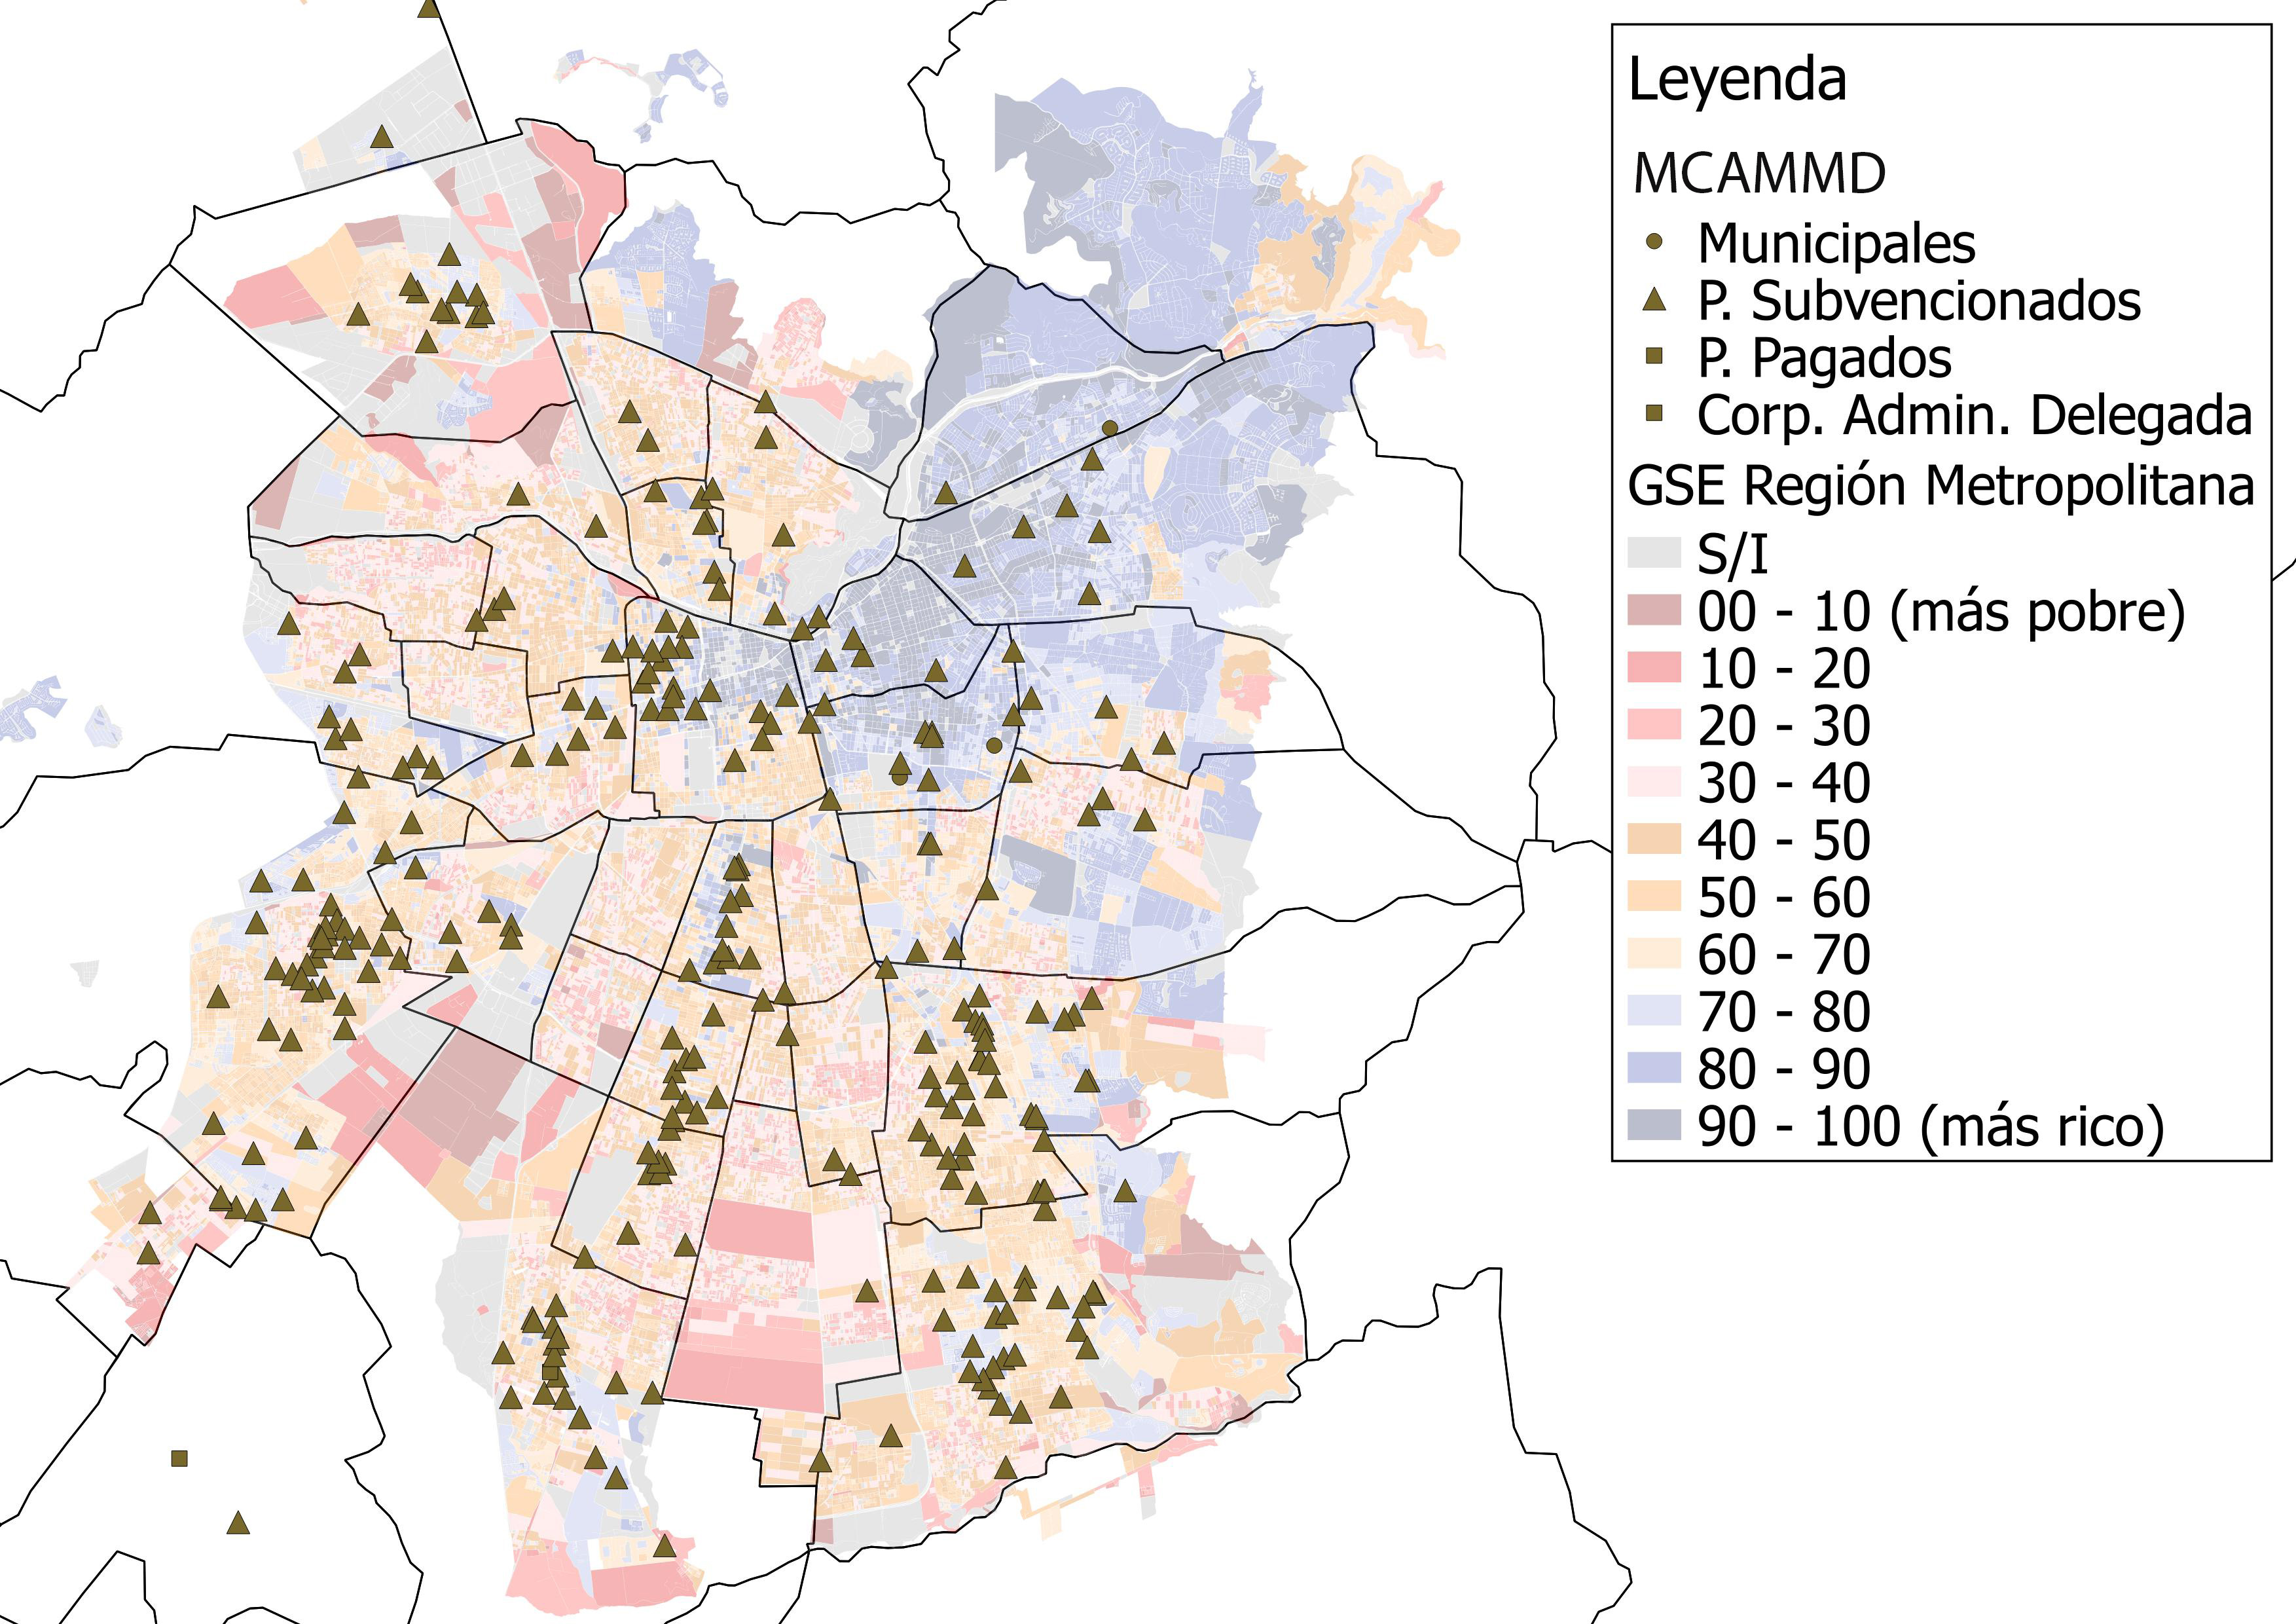
\includegraphics[width=7.5cm]{images/establecimientos/E_TODOS_CON_2.jpg}}
  \subfloat[Establecimientos clúster E\_TODOS\_CON\_3.]{
   \label{f:}
    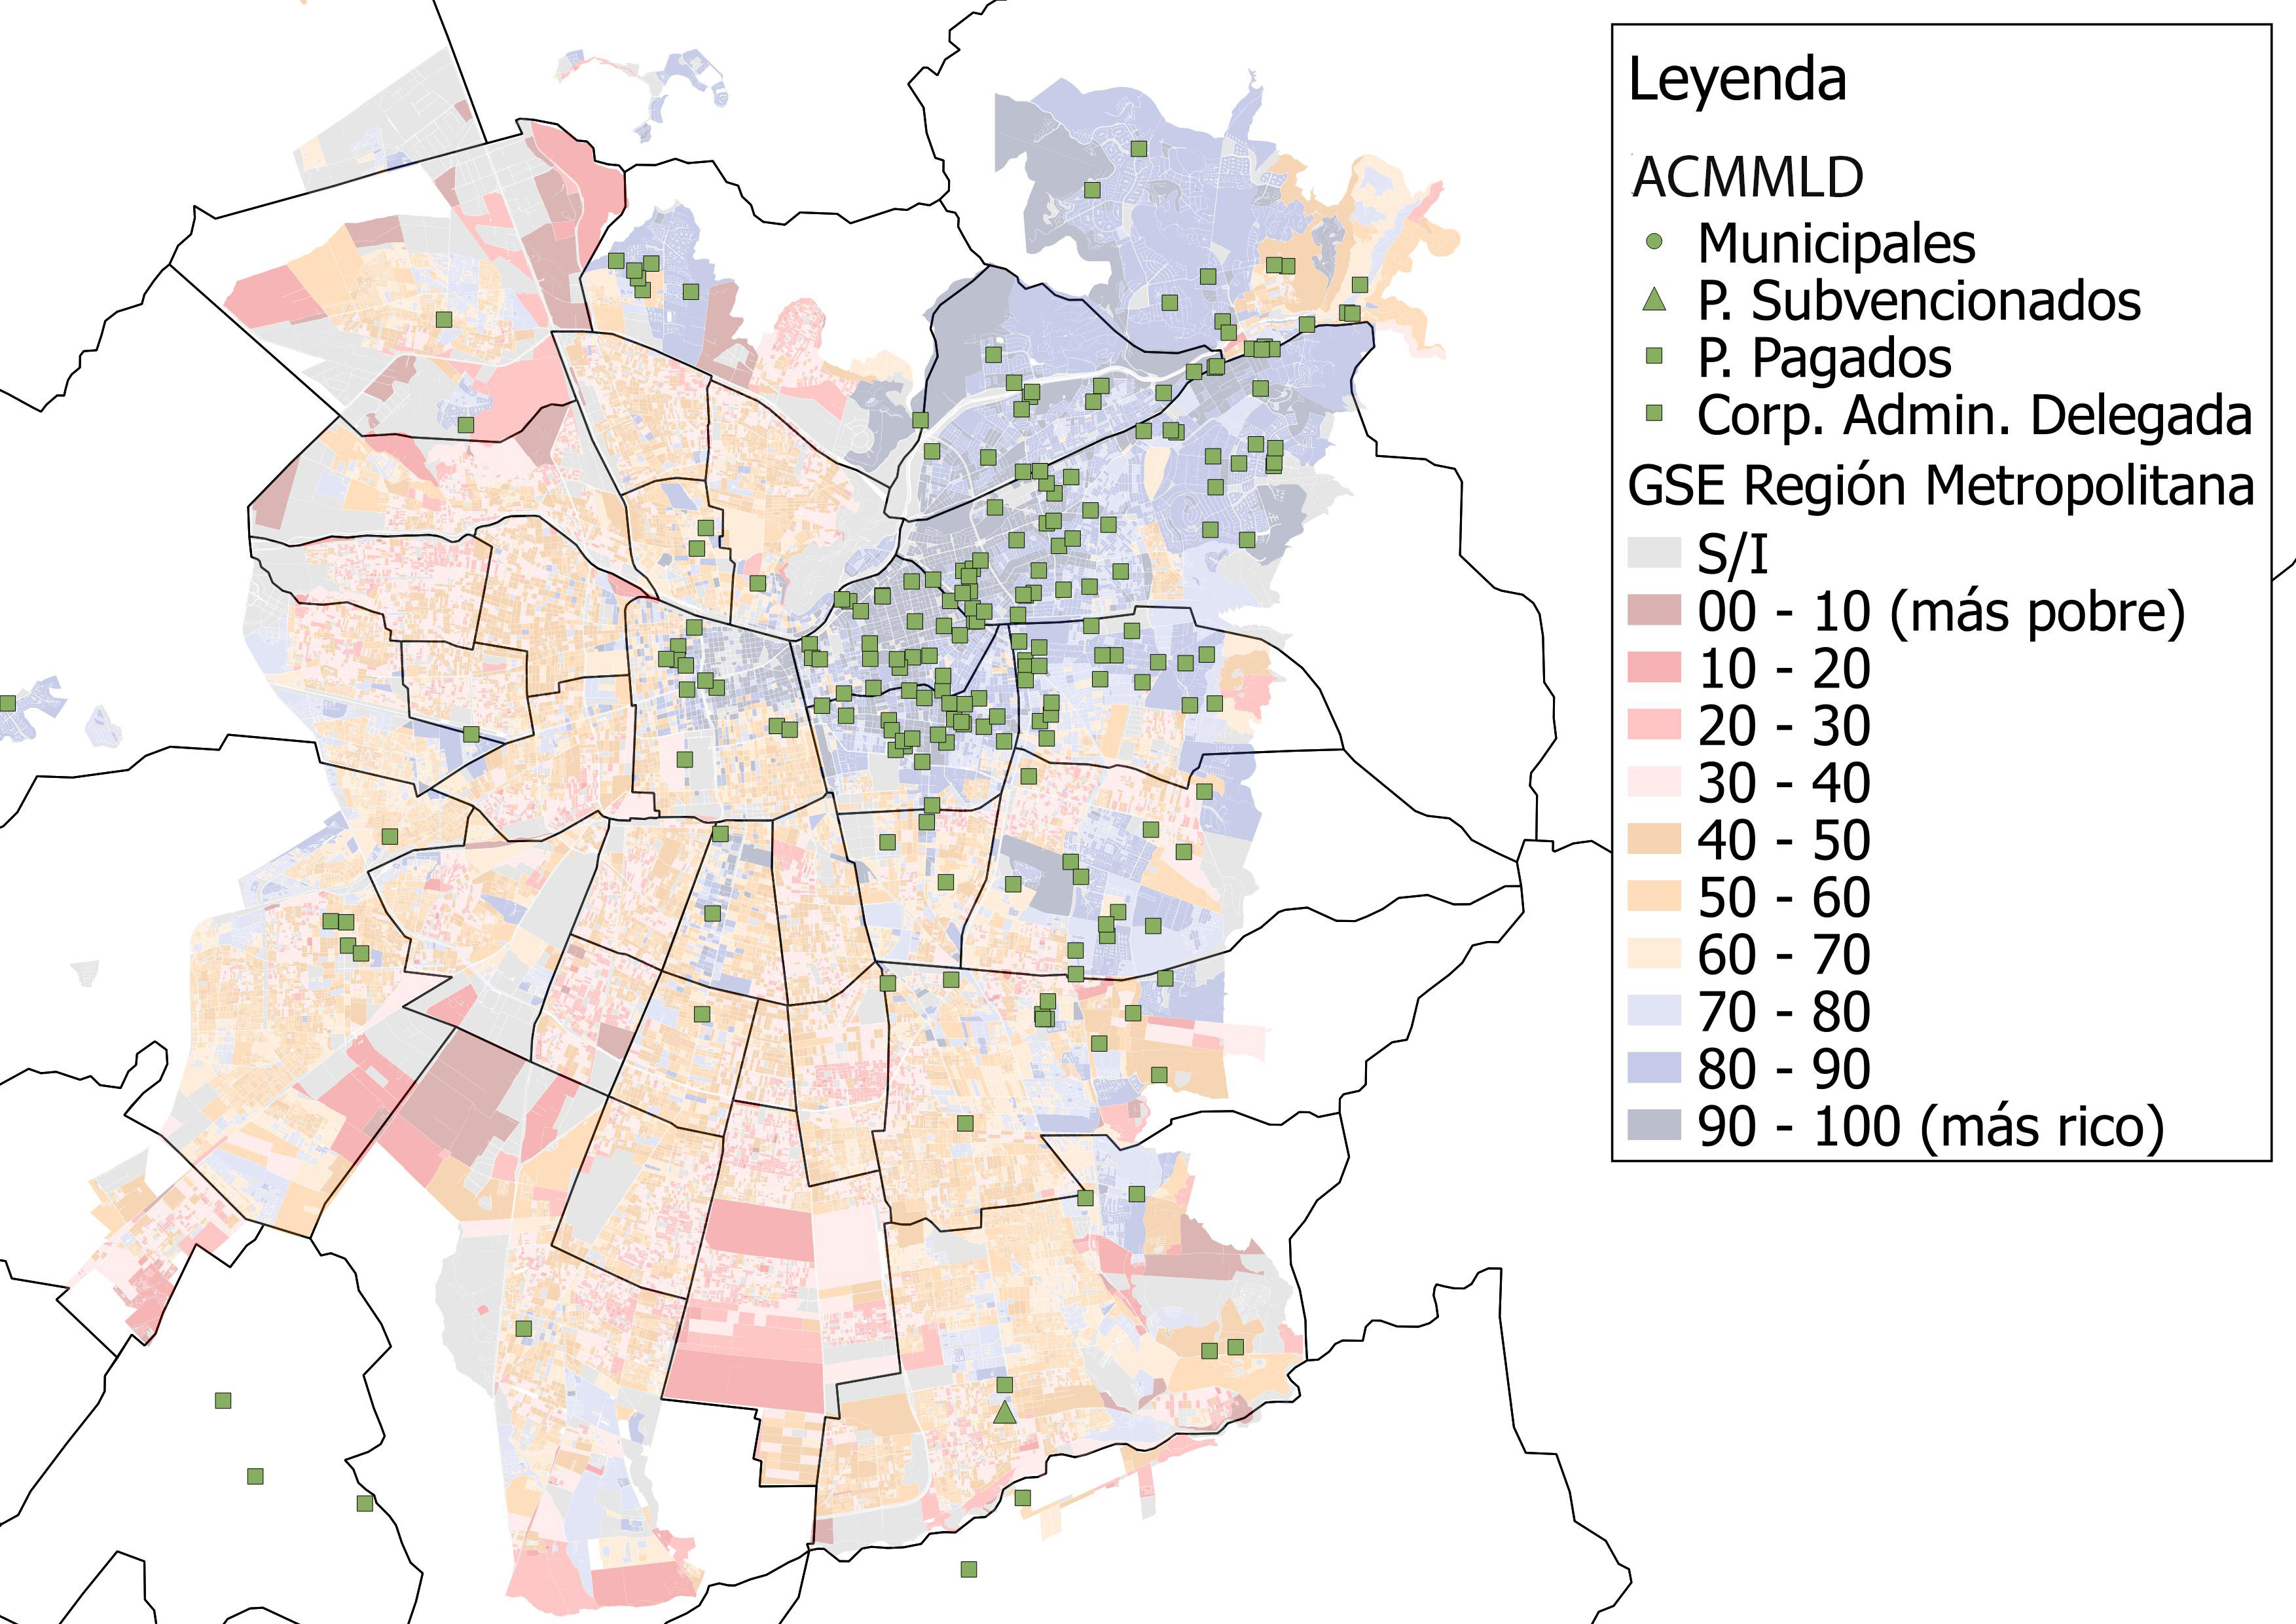
\includegraphics[width=7.5cm]{images/establecimientos/E_TODOS_CON_3.jpg}}
 \caption{Mapas de clústers de establecimientos (con atributos relacionales) sobre mapa GSE de la Región Metropolitana.}
 \label{f:}
\end{figure}

\begin{figure}[H]
 \centering
  \subfloat[Matrículas en colegios de E\_TODOS\_SIN\_0.]{
   \label{f:}
    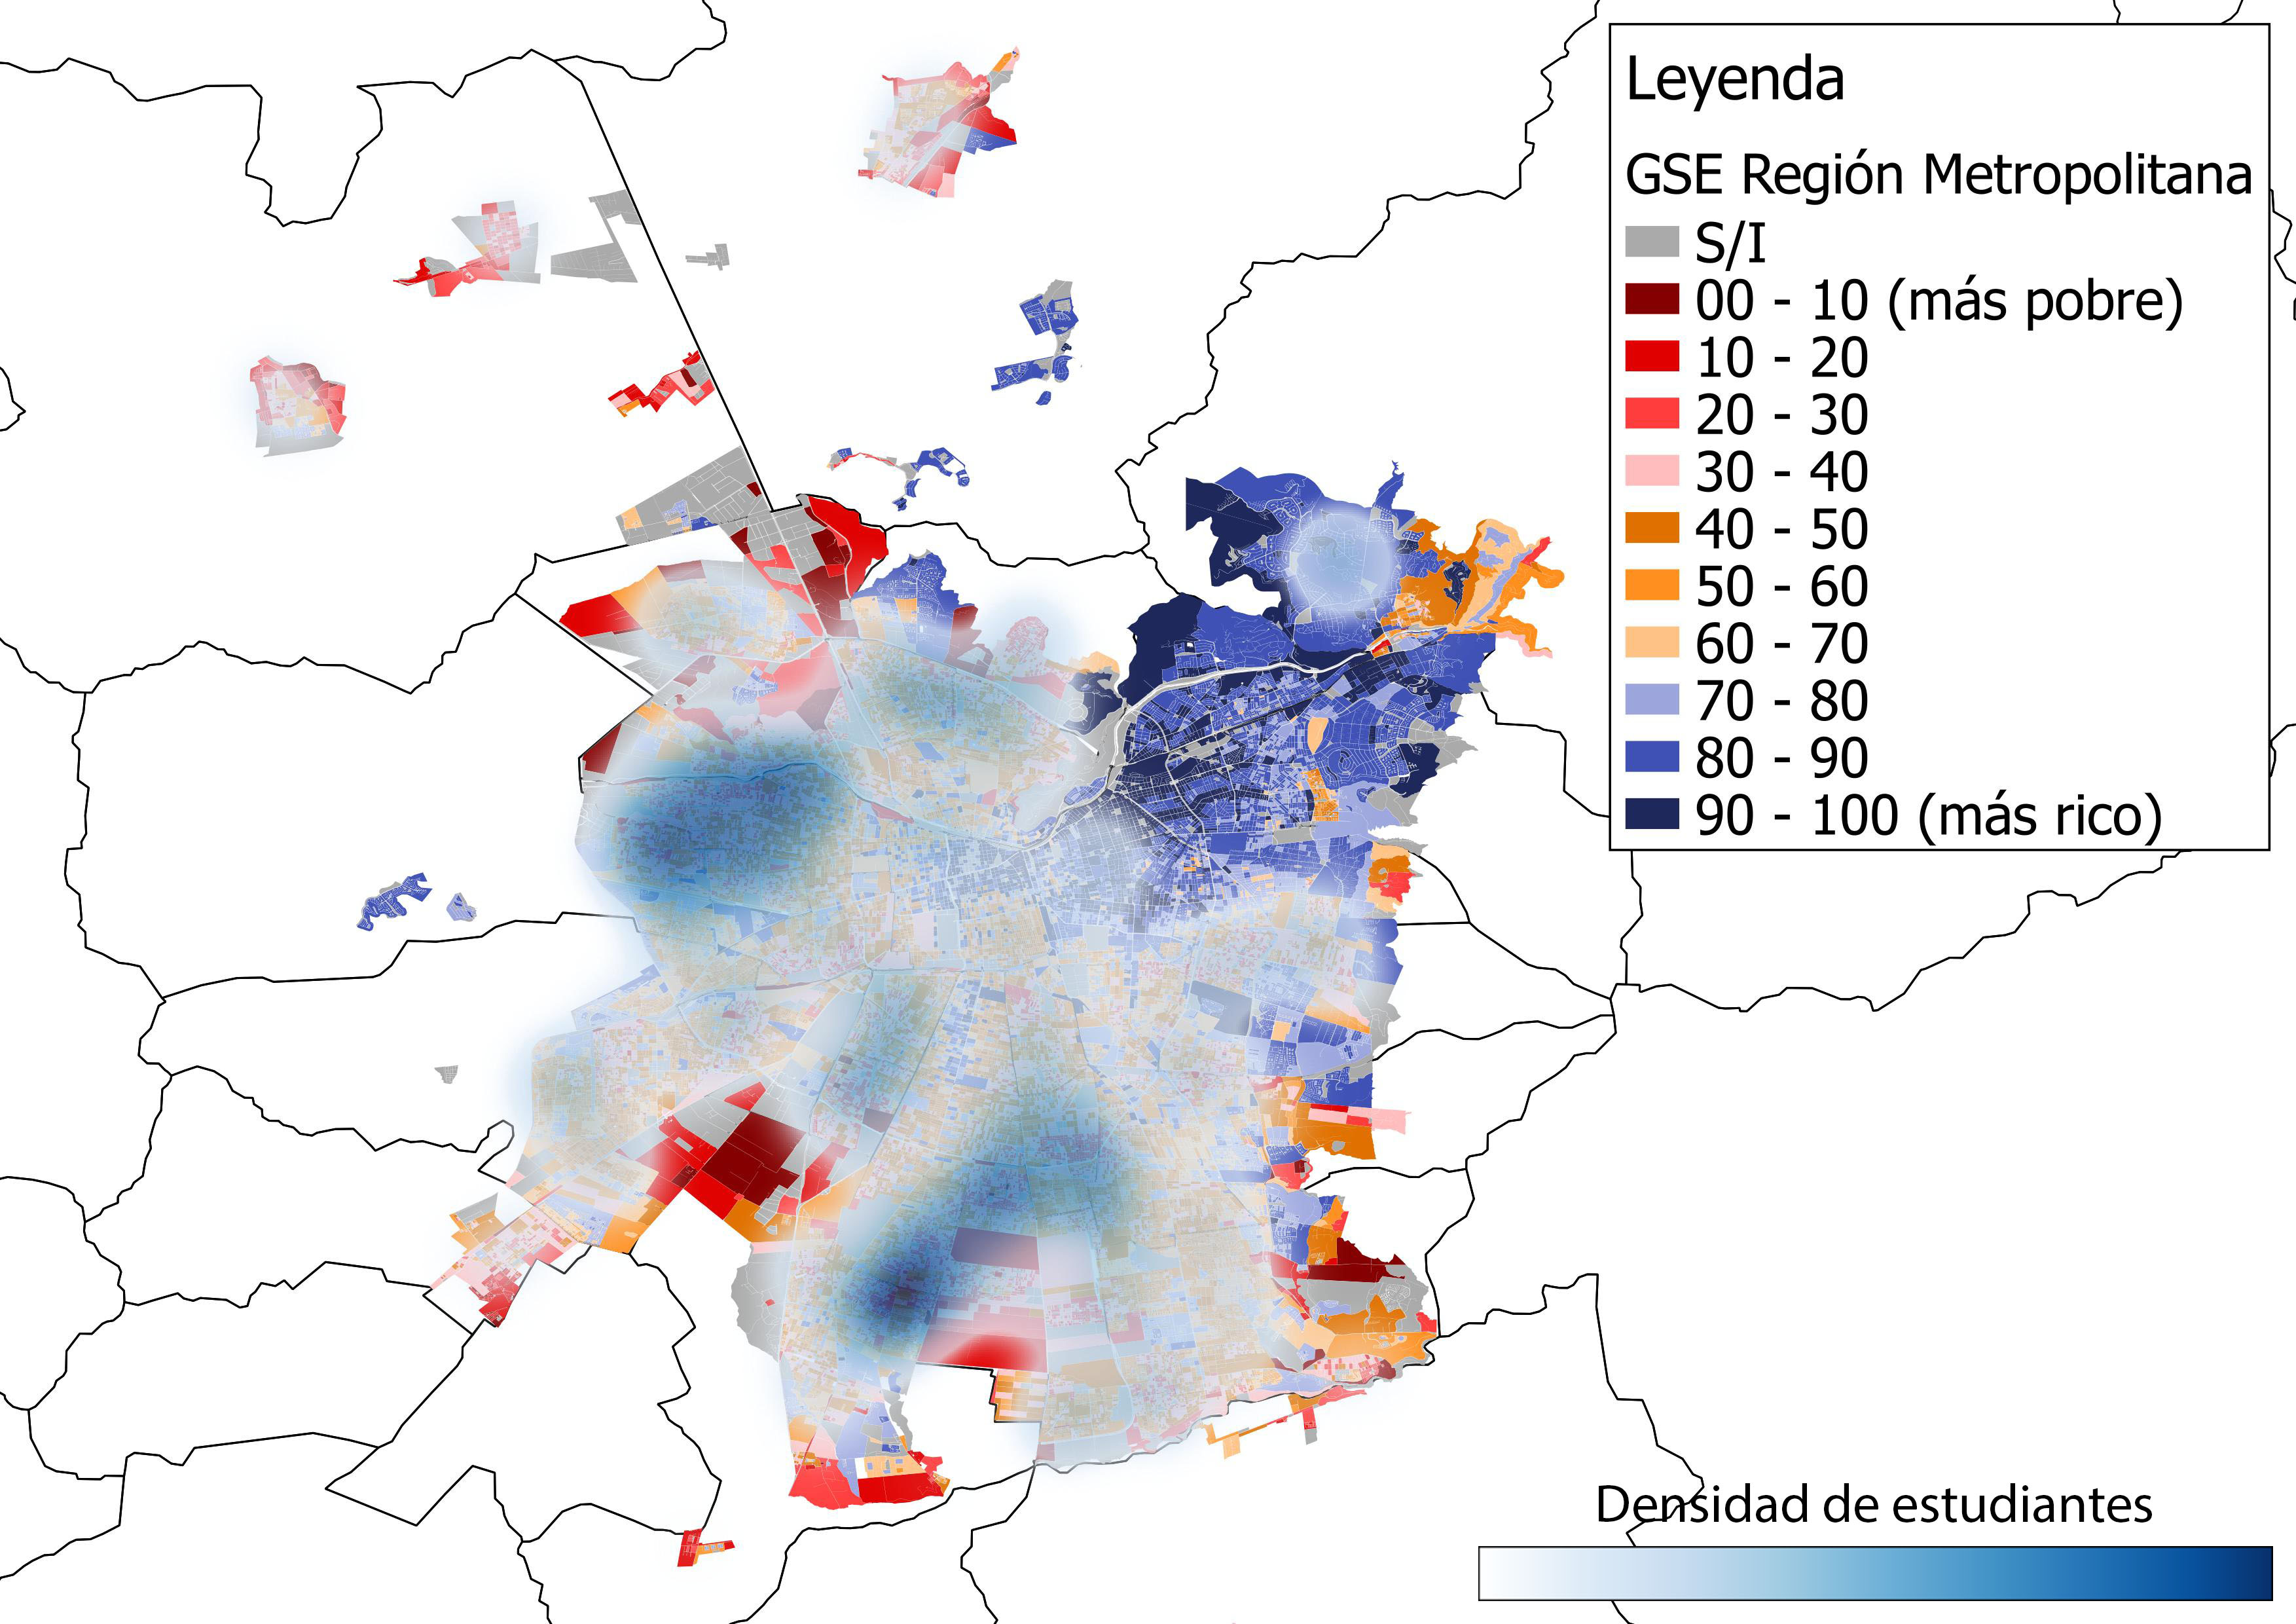
\includegraphics[width=7.5cm]{images/matriculas/E_SIN_0_final.jpg}}
  \subfloat[Matrículas en colegios de E\_TODOS\_SIN\_1.]{
   \label{f:}
    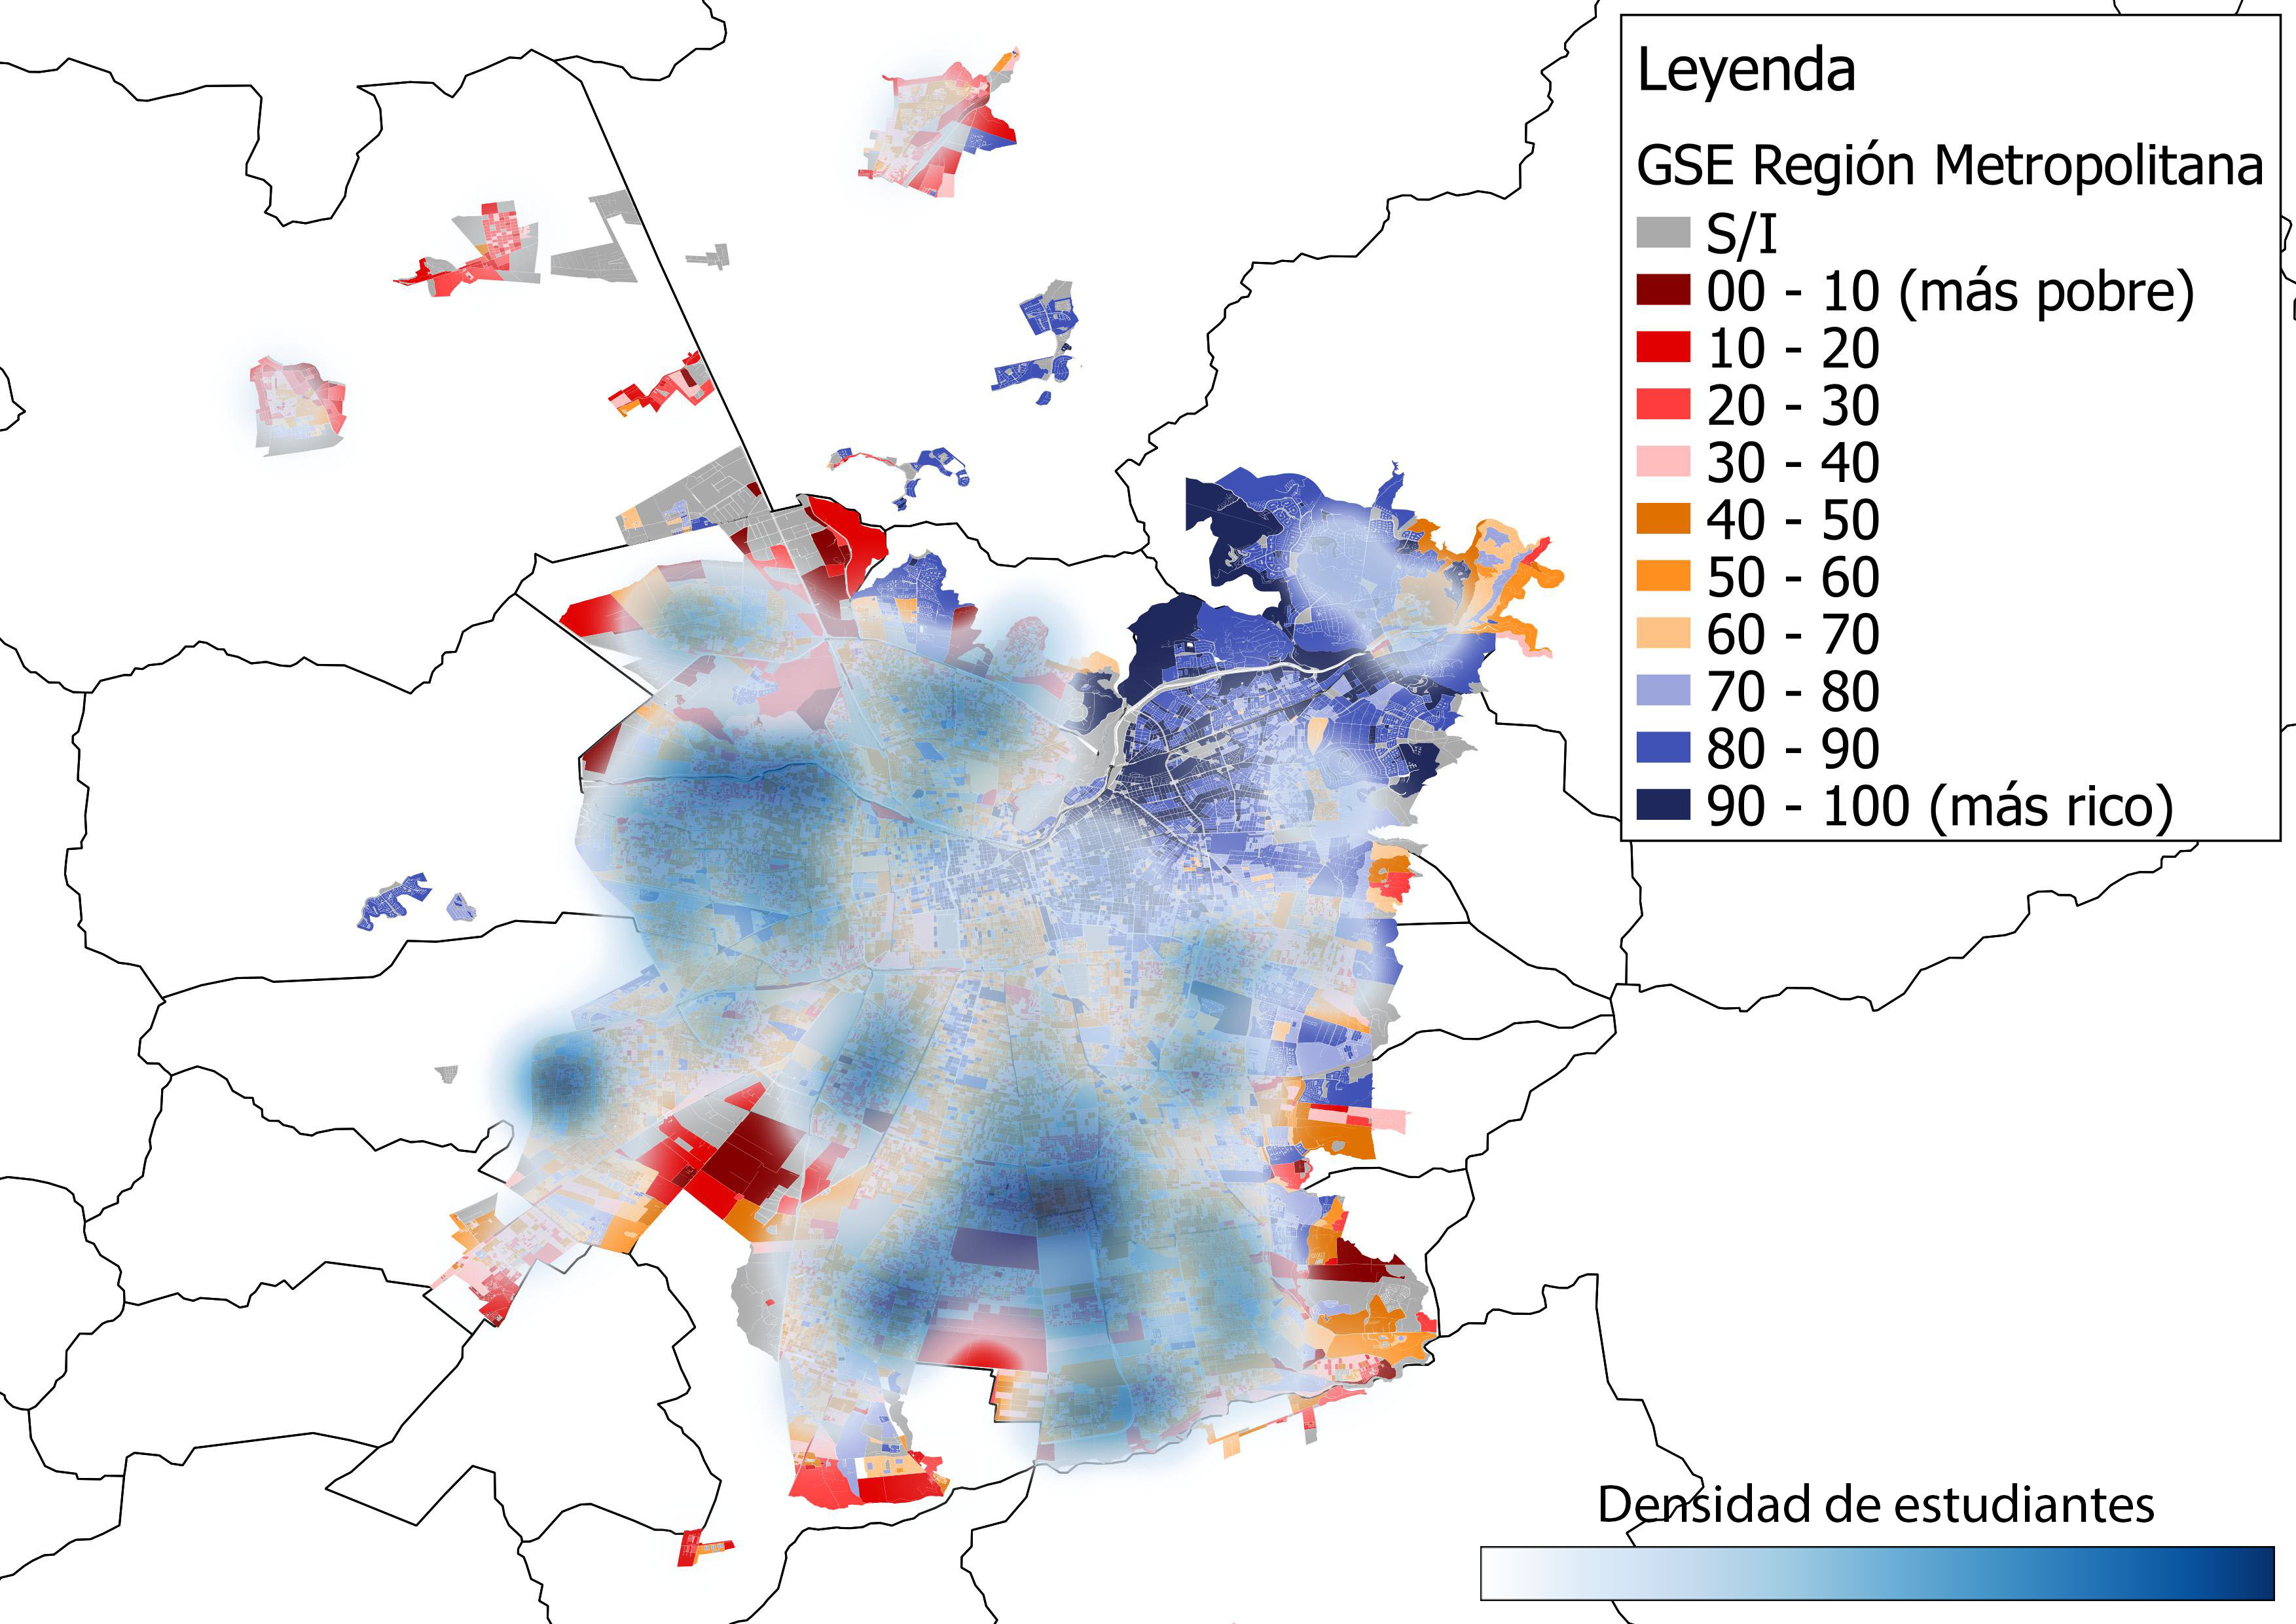
\includegraphics[width=7.5cm]{images/matriculas/E_SIN_1_final.jpg}}\hspace{1mm}
  \subfloat[Matrículas en colegios de E\_TODOS\_SIN\_2.]{
   \label{f:}
    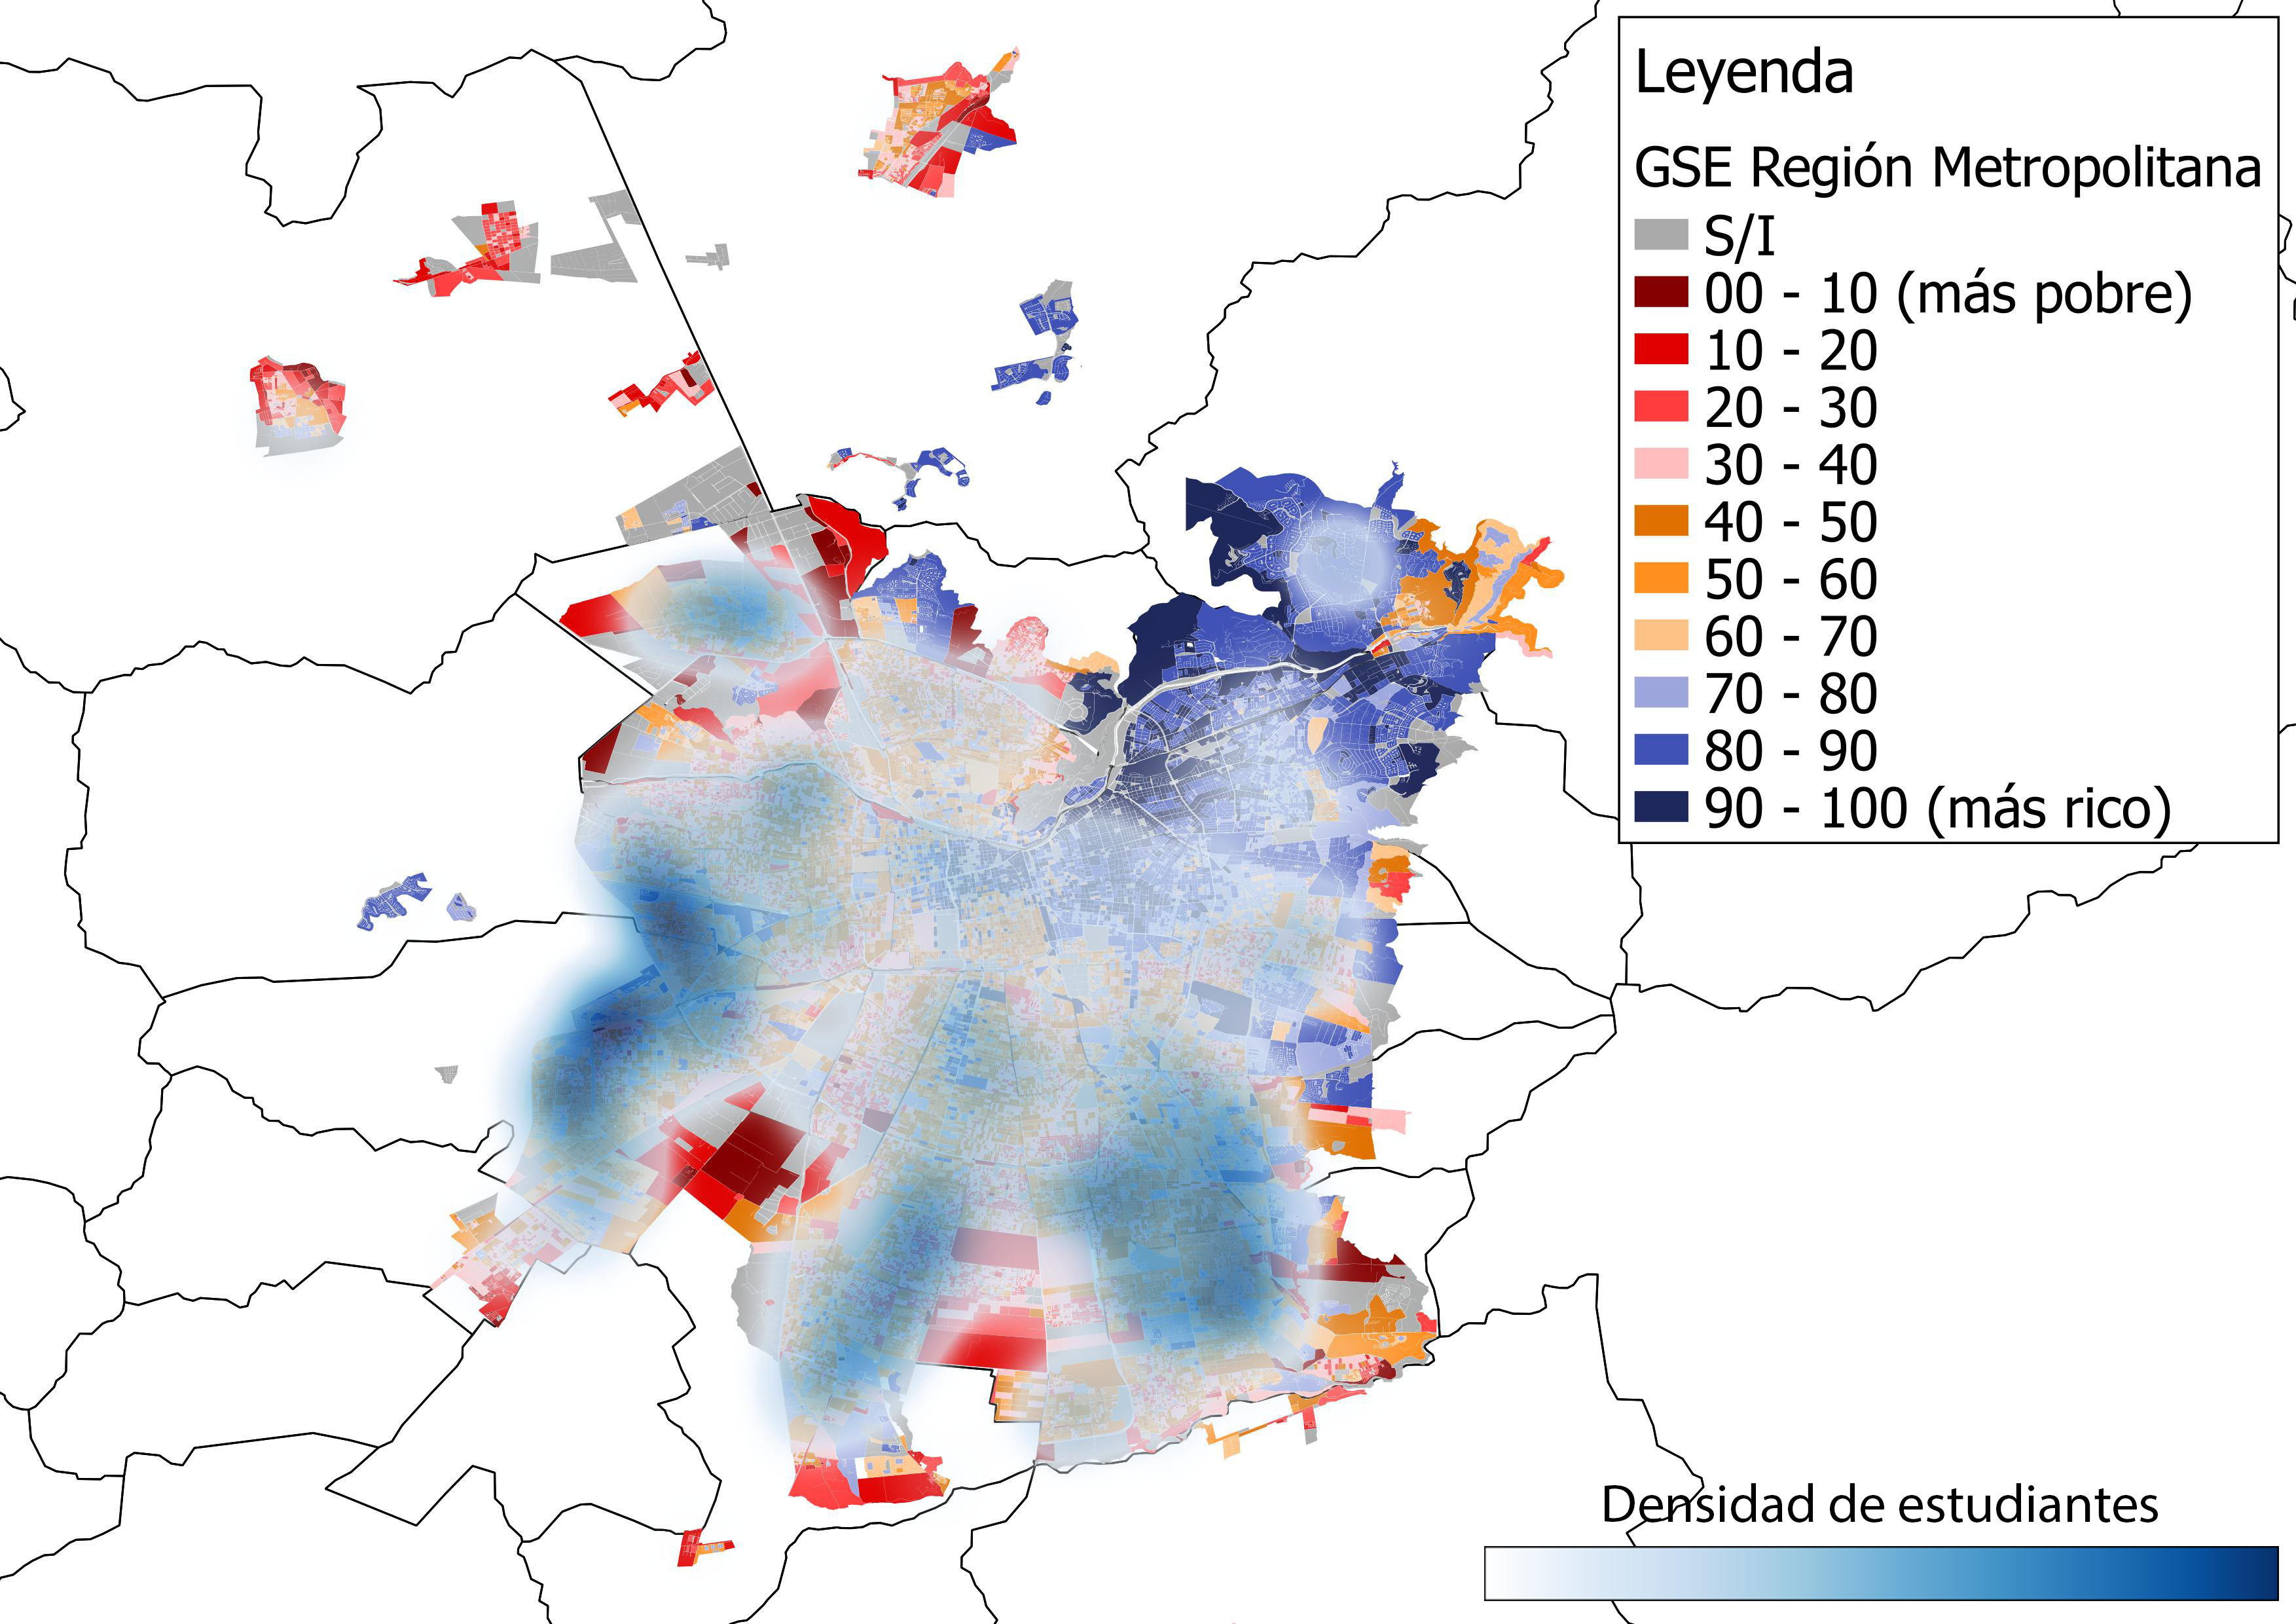
\includegraphics[width=7.5cm]{images/matriculas/E_SIN_2_final.jpg}}
  \subfloat[Matrículas en colegios de E\_TODOS\_SIN\_3.]{
   \label{f:}
    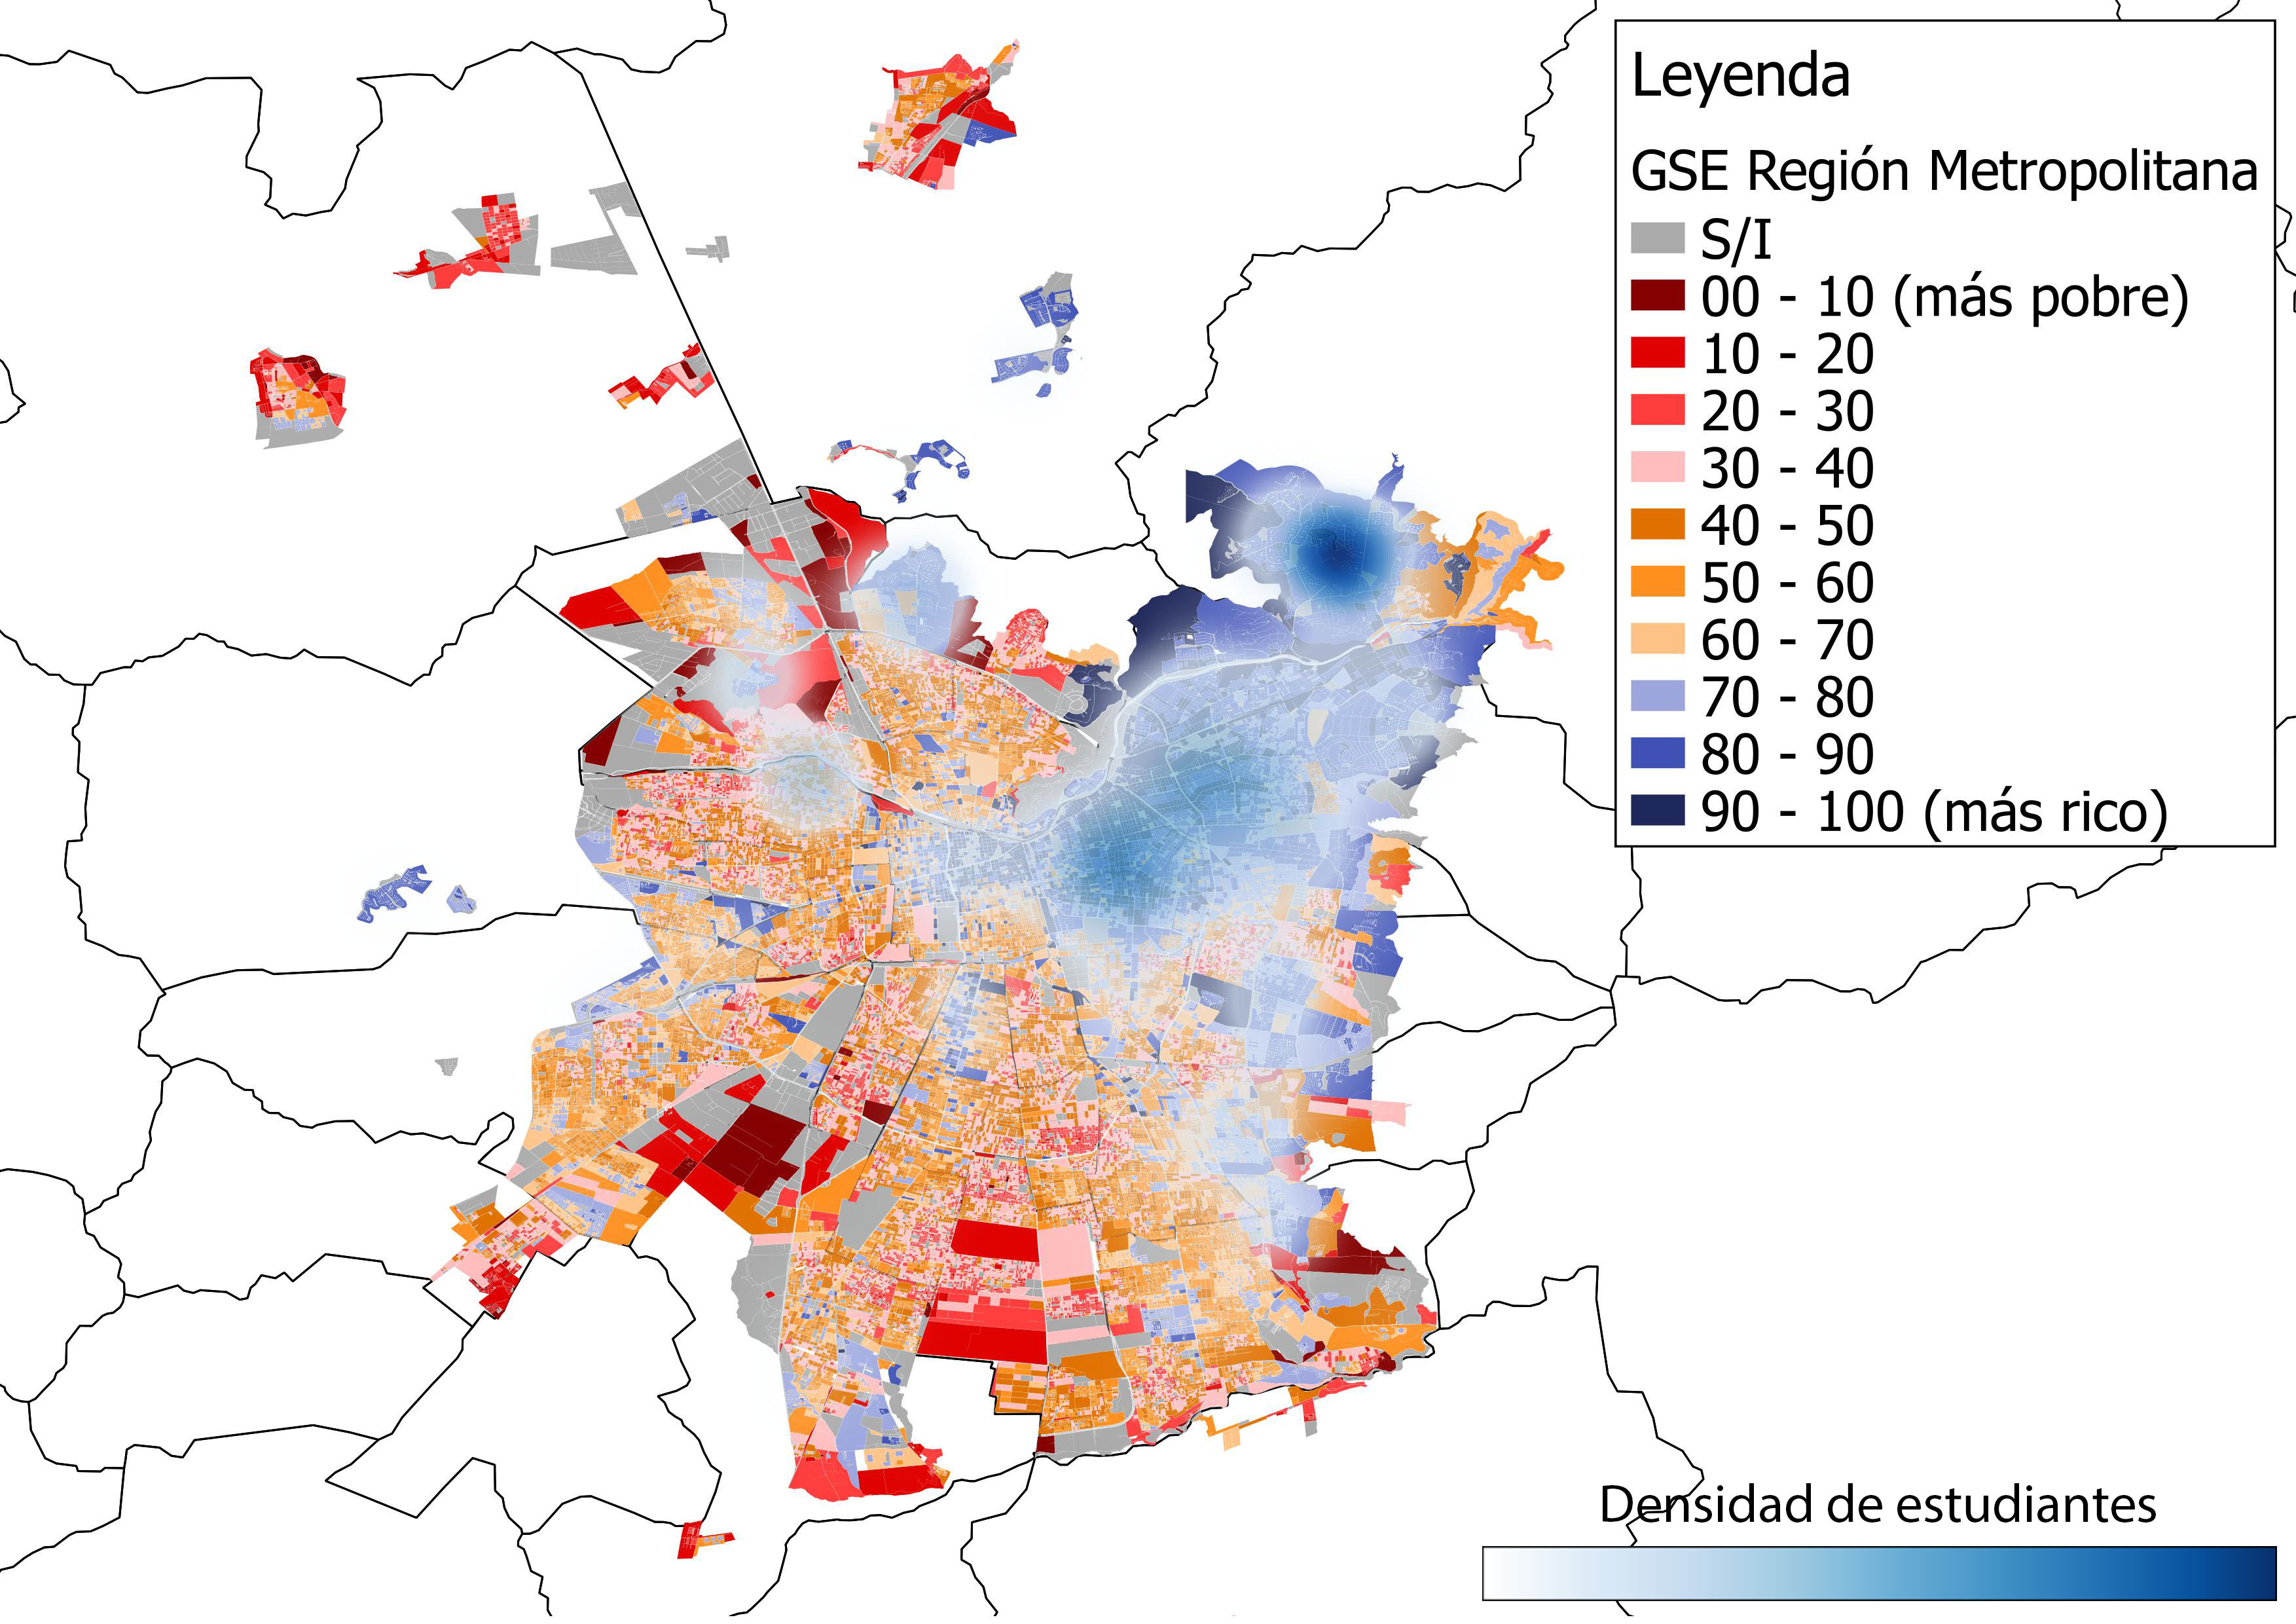
\includegraphics[width=7.5cm]{images/matriculas/E_SIN_3_final.jpg}}
 \caption{Mapas de calor de matrículas en clústers de establecimientos sobre mapa GSE de la Región Metropolitana.}
 \label{f:}
\end{figure}

\begin{figure}[H]
 \centering
  \subfloat[Matrículas clúster M\_TODAS\_SIN\_0.]{
   \label{f:}
    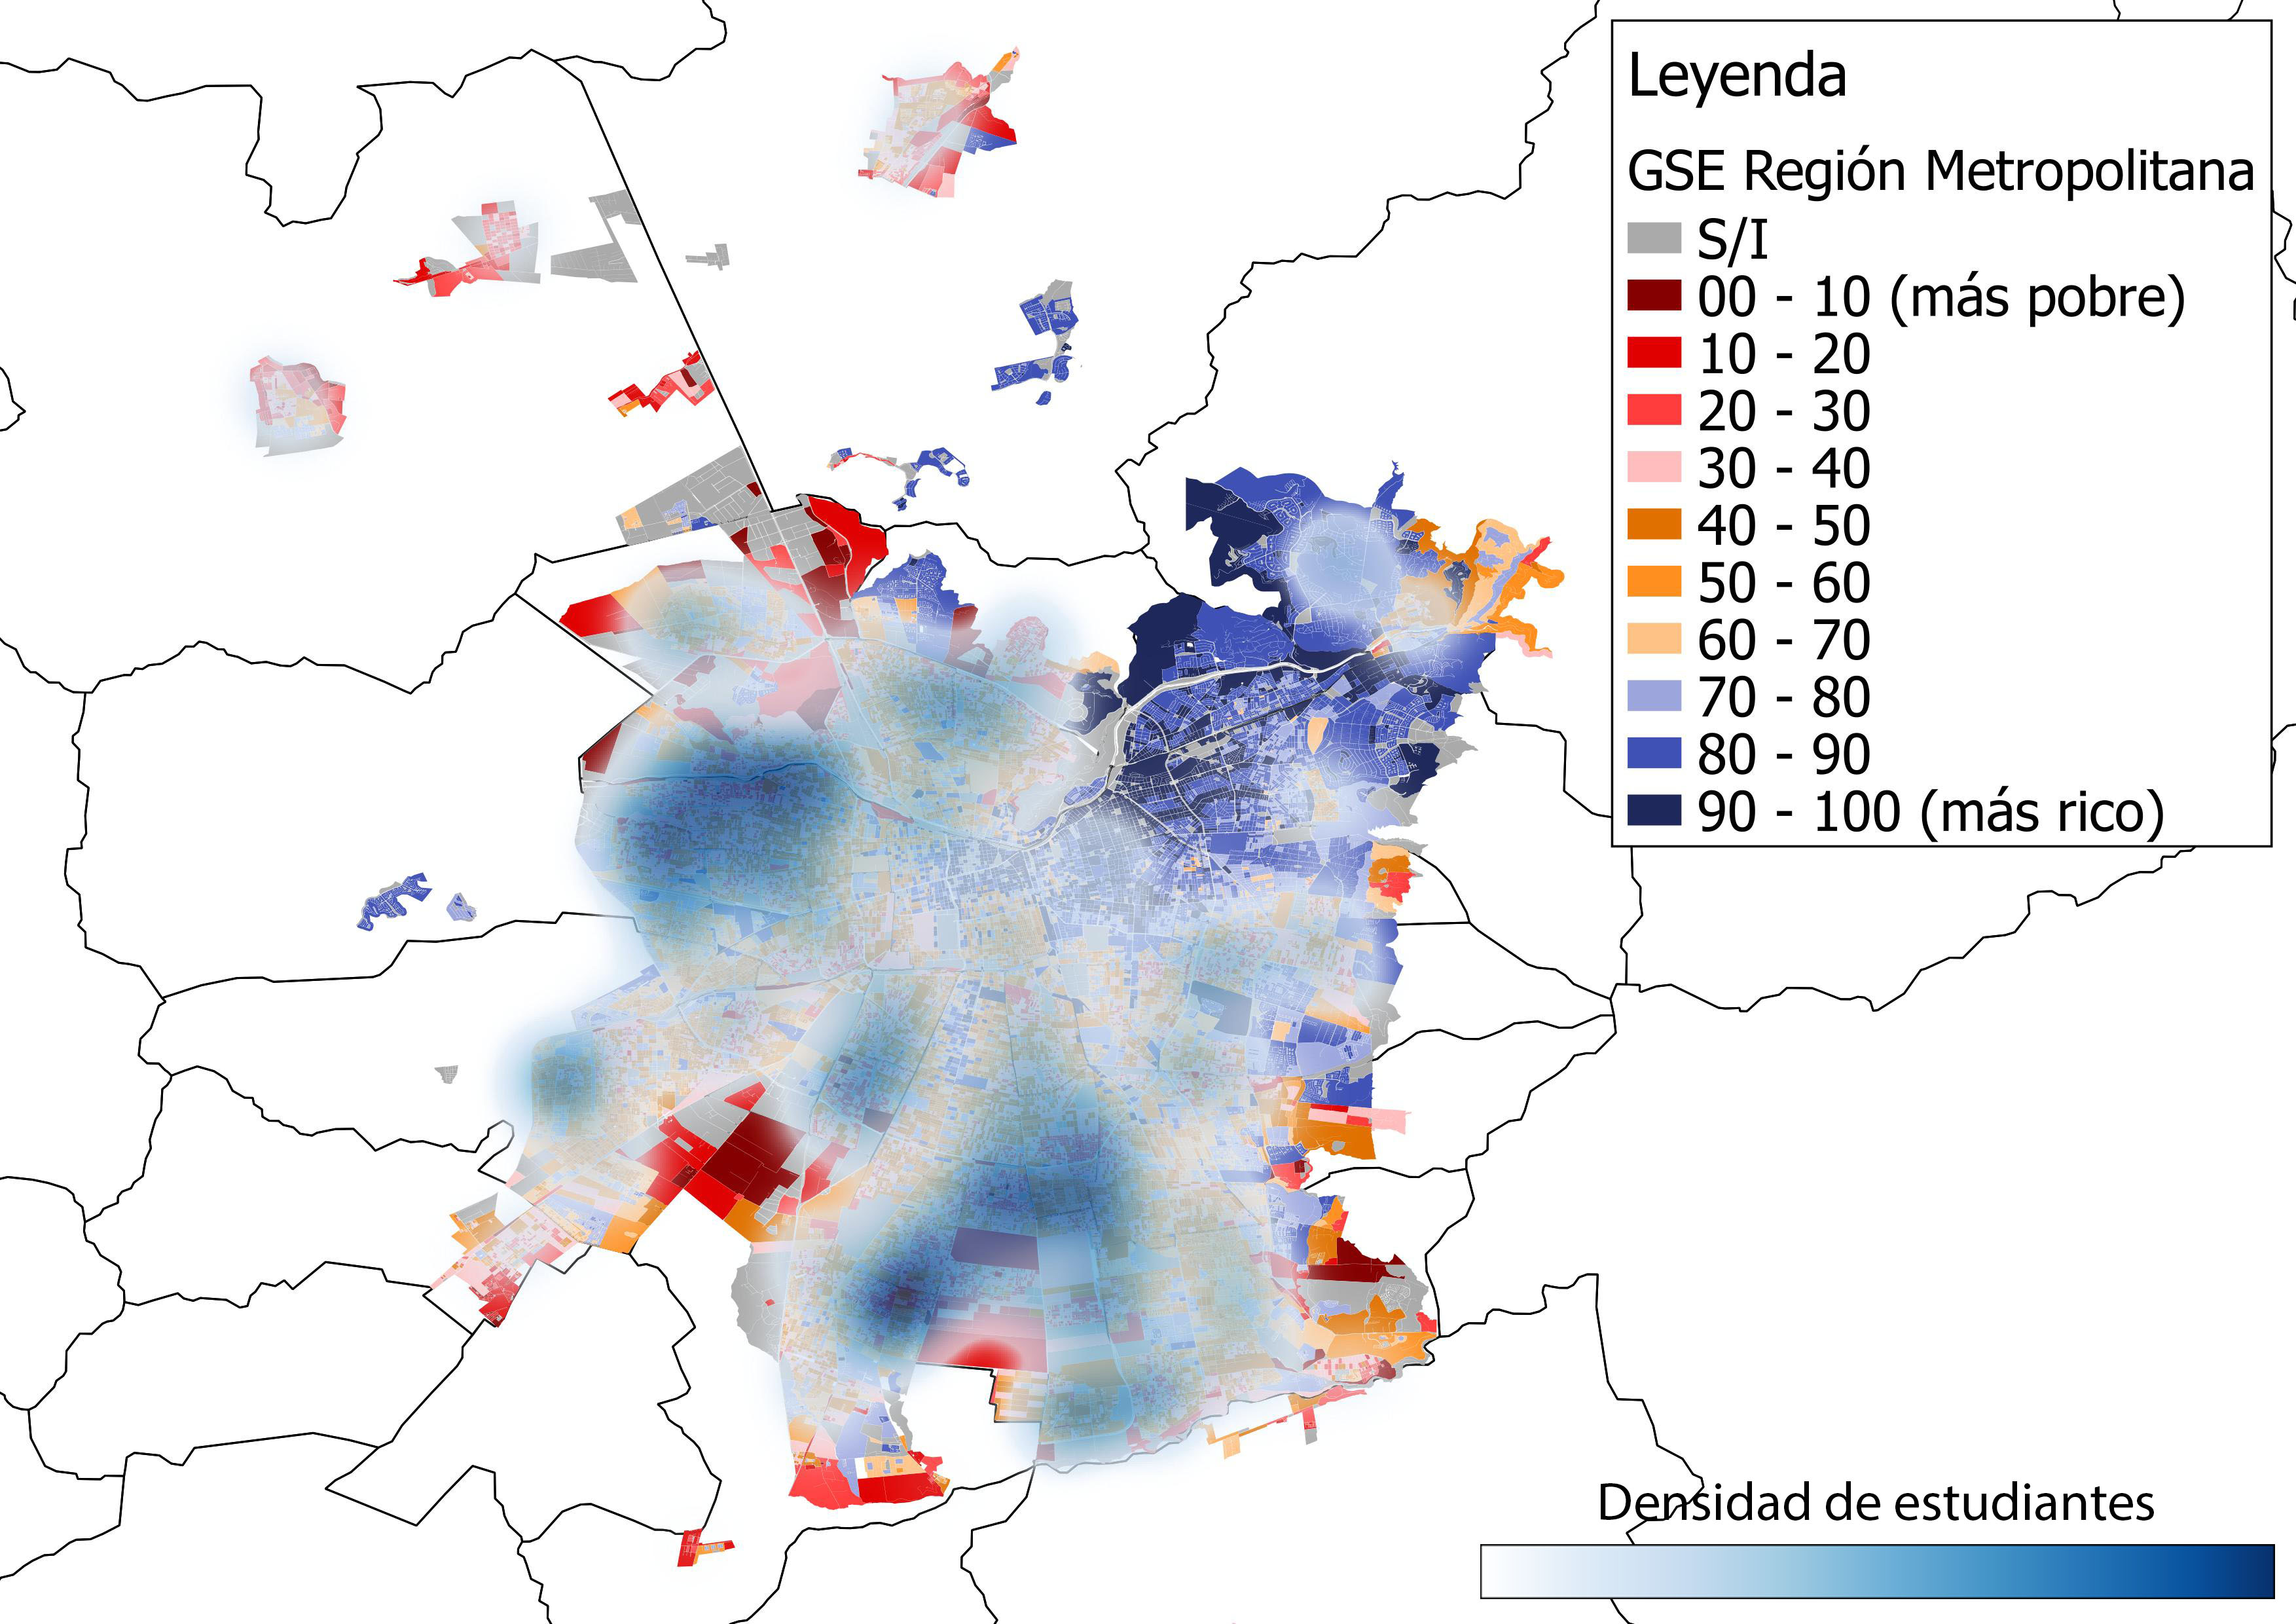
\includegraphics[width=7.5cm]{images/matriculas/M_SIN_0_final.jpg}}
  \subfloat[Matrículas clúster M\_TODAS\_SIN\_1.]{
   \label{f:}
    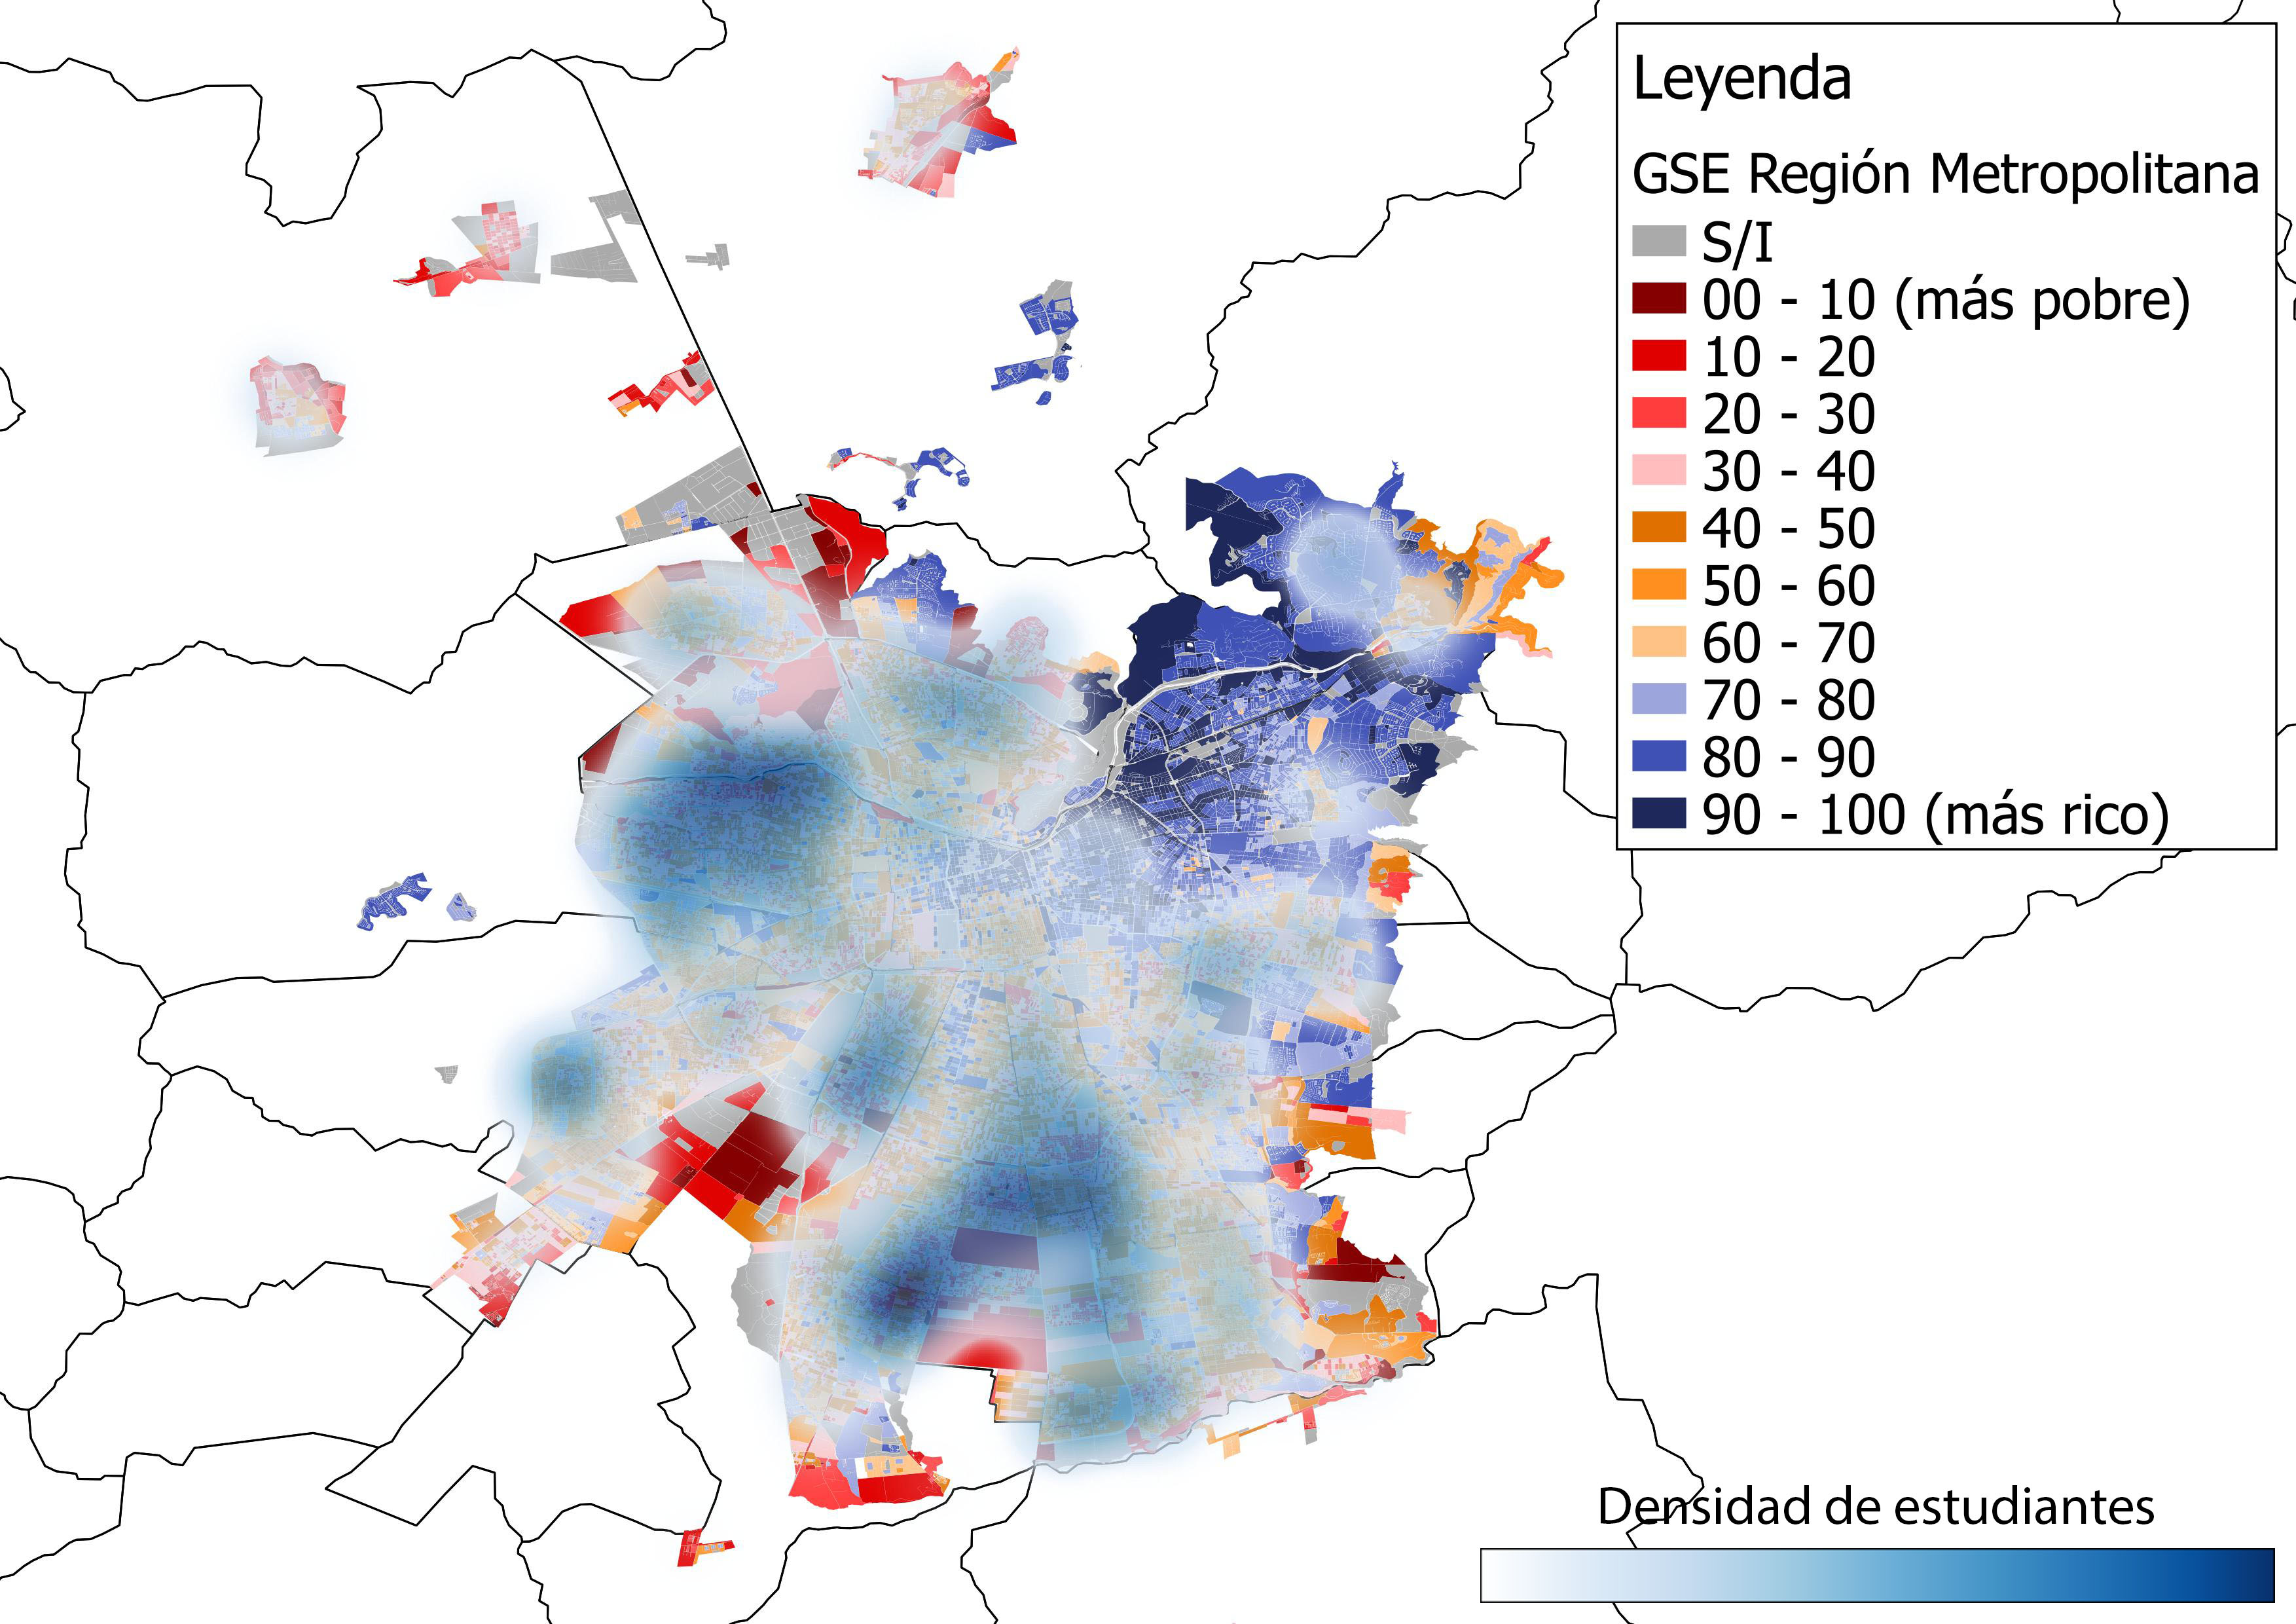
\includegraphics[width=7.5cm]{images/matriculas/M_SIN_1_final.jpg}}\hspace{1mm}
  \subfloat[Matrículas clúster M\_TODAS\_SIN\_2.]{
   \label{f:}
    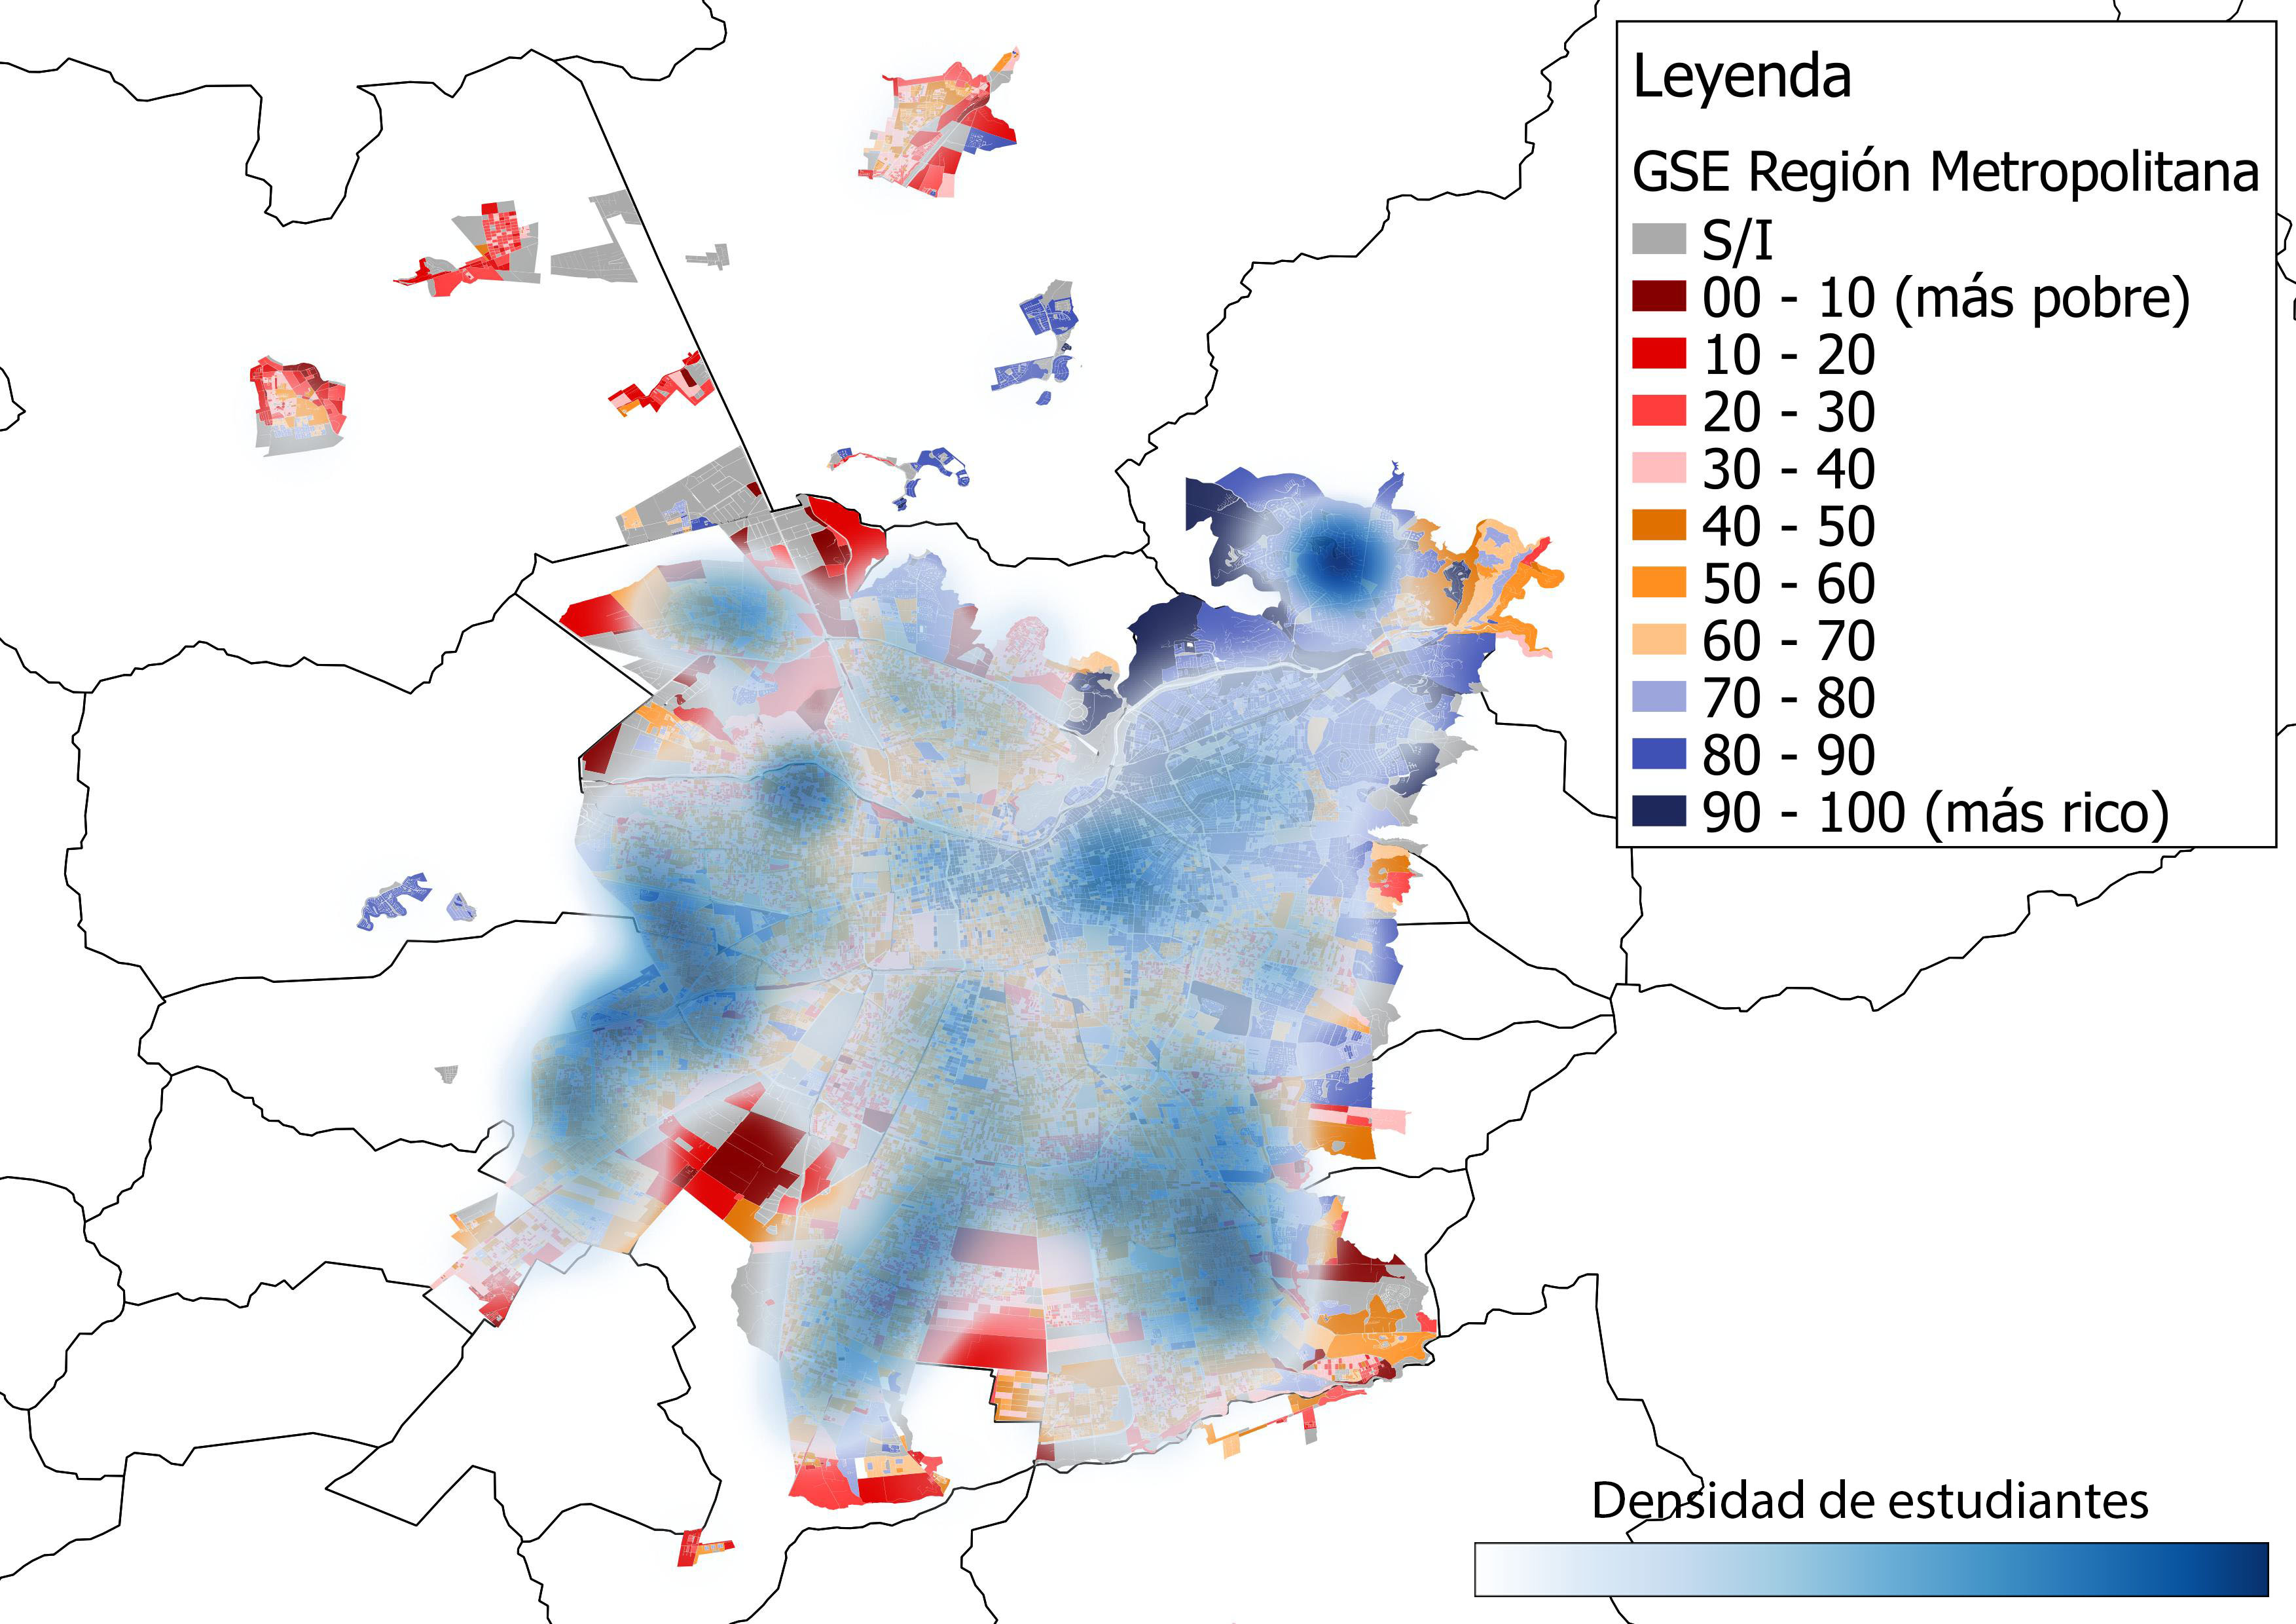
\includegraphics[width=7.5cm]{images/matriculas/M_SIN_2_final.jpg}}
  \subfloat[Matrículas clúster M\_TODAS\_SIN\_3.]{
   \label{f:}
    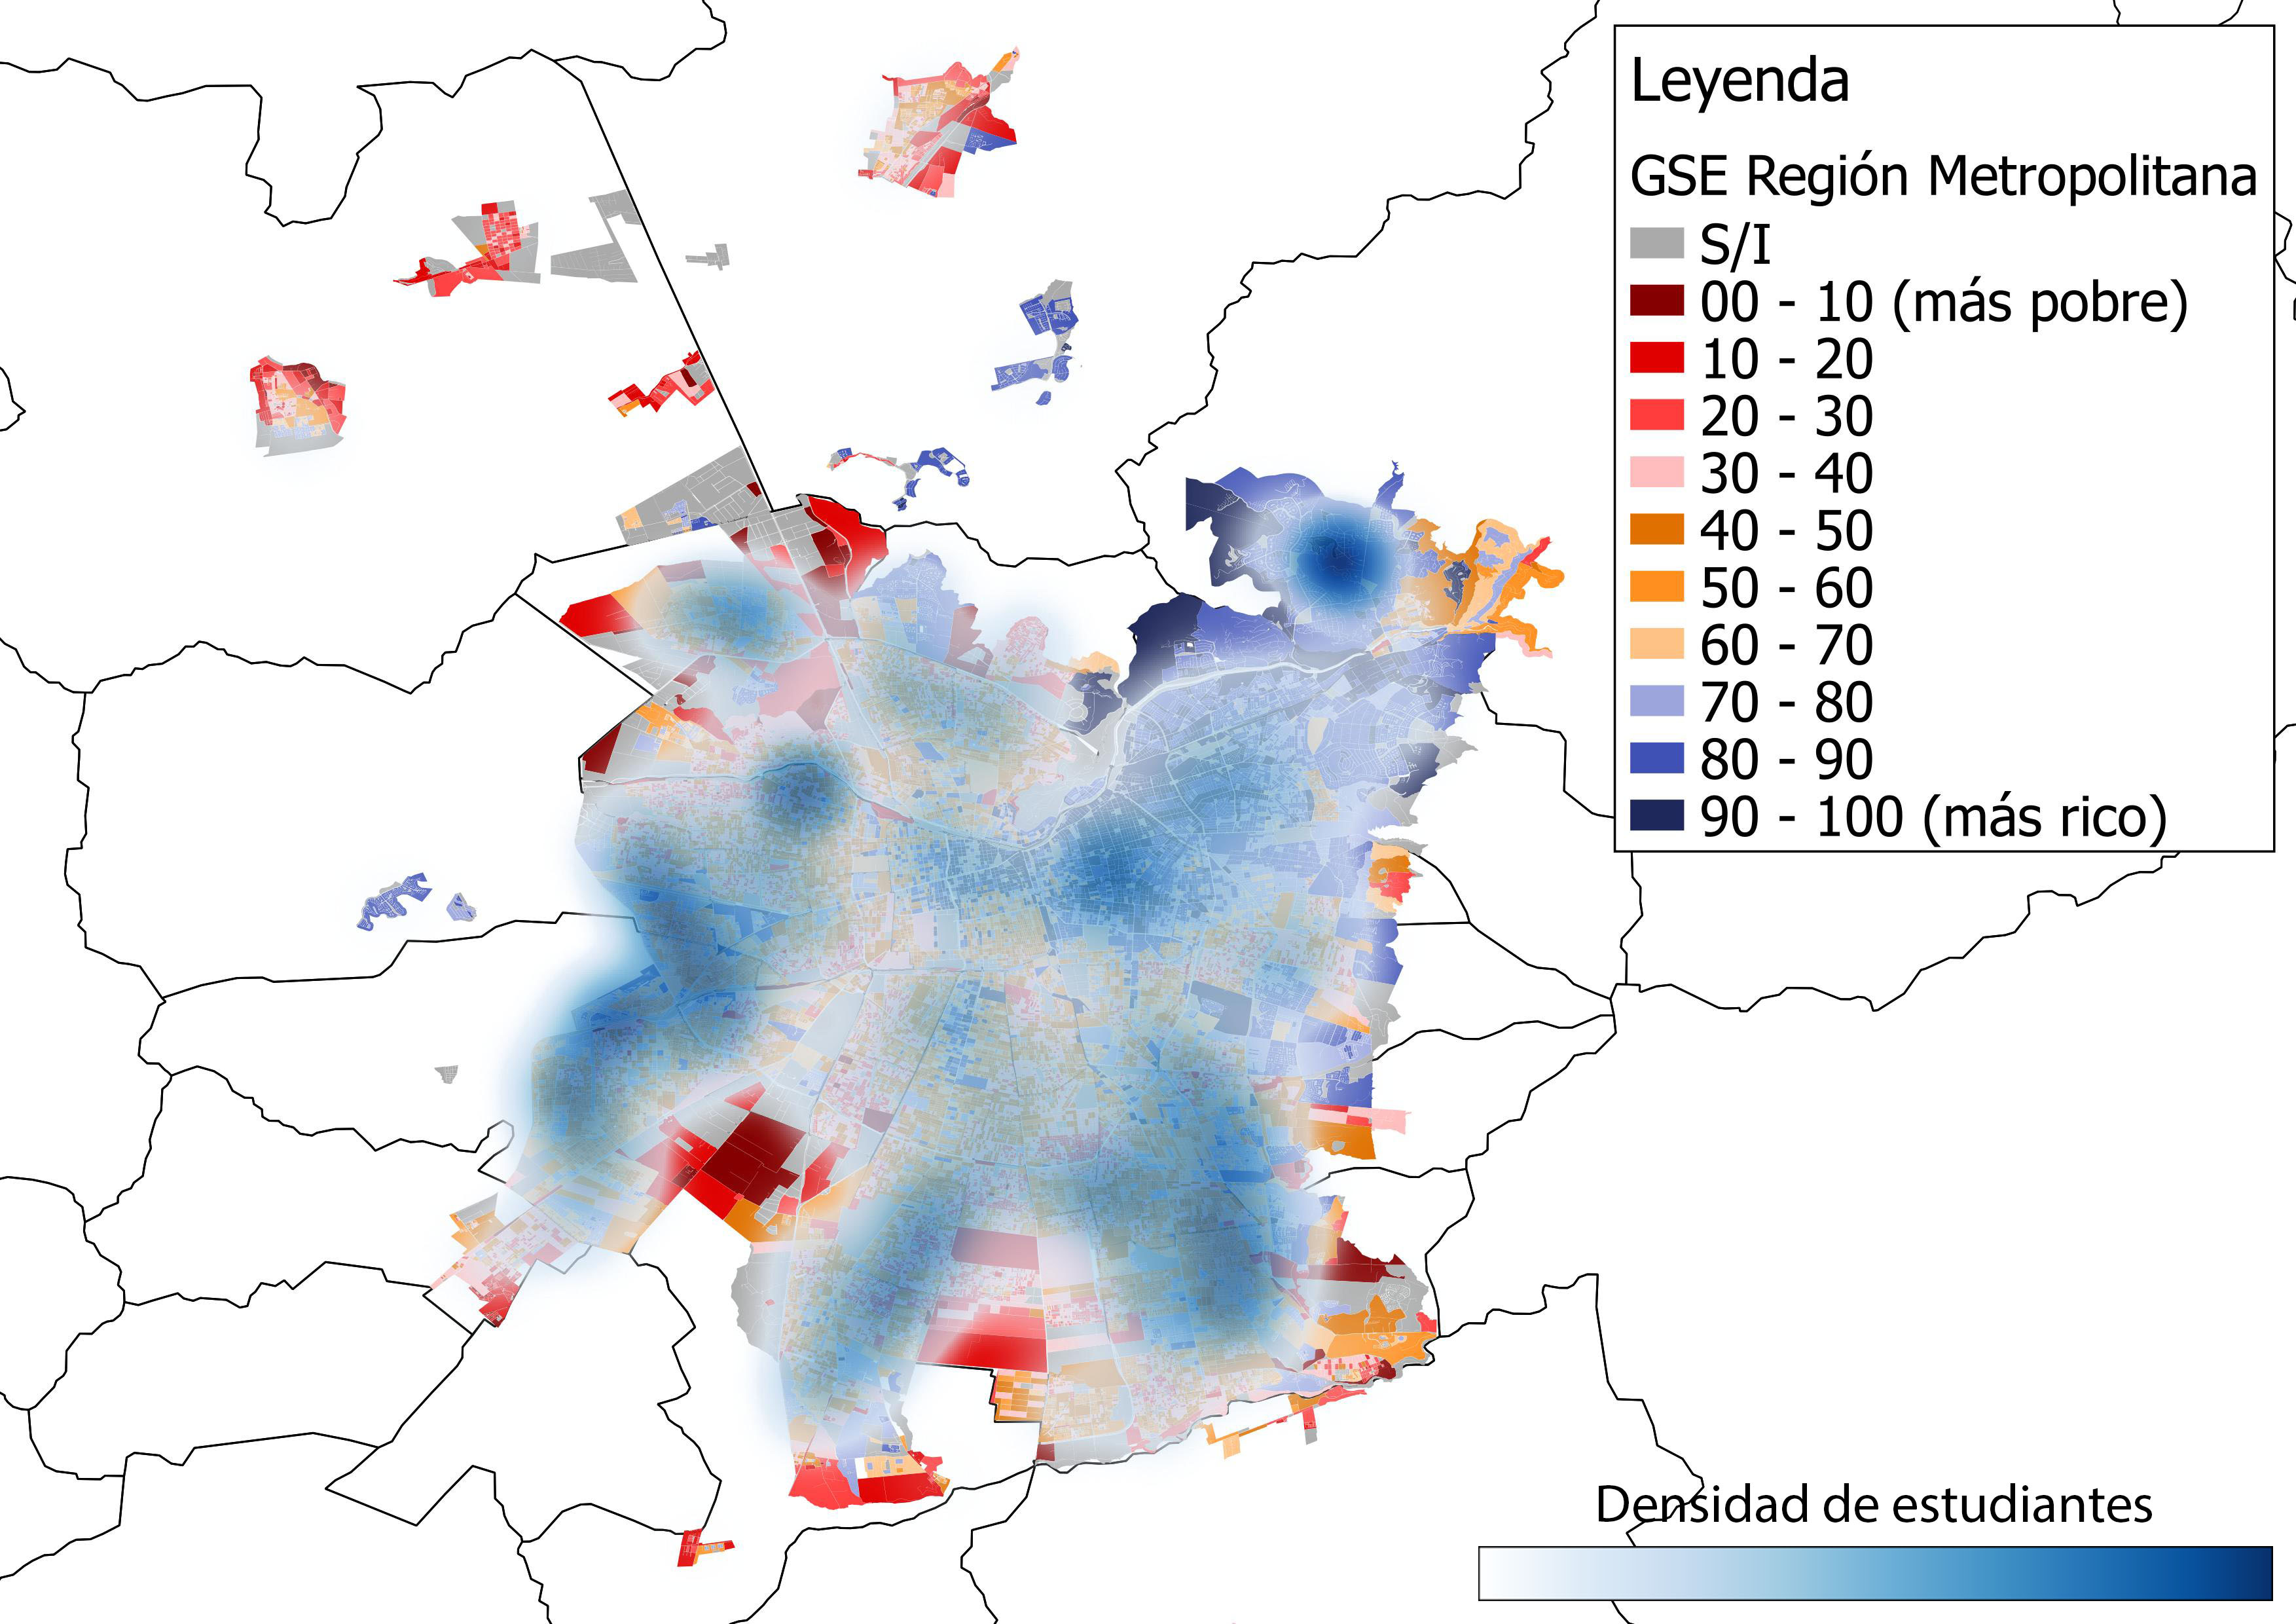
\includegraphics[width=7.5cm]{images/matriculas/M_SIN_3_final.jpg}}
 \caption{Mapas de calor de clústers de matrículas sobre mapa GSE de la Región Metropolitana.}
 \label{f:}
\end{figure}

\begin{figure}[H]
 \centering
  \subfloat[Matrículas en colegios de E\_TODOS\_CON\_0.]{
   \label{f:}
    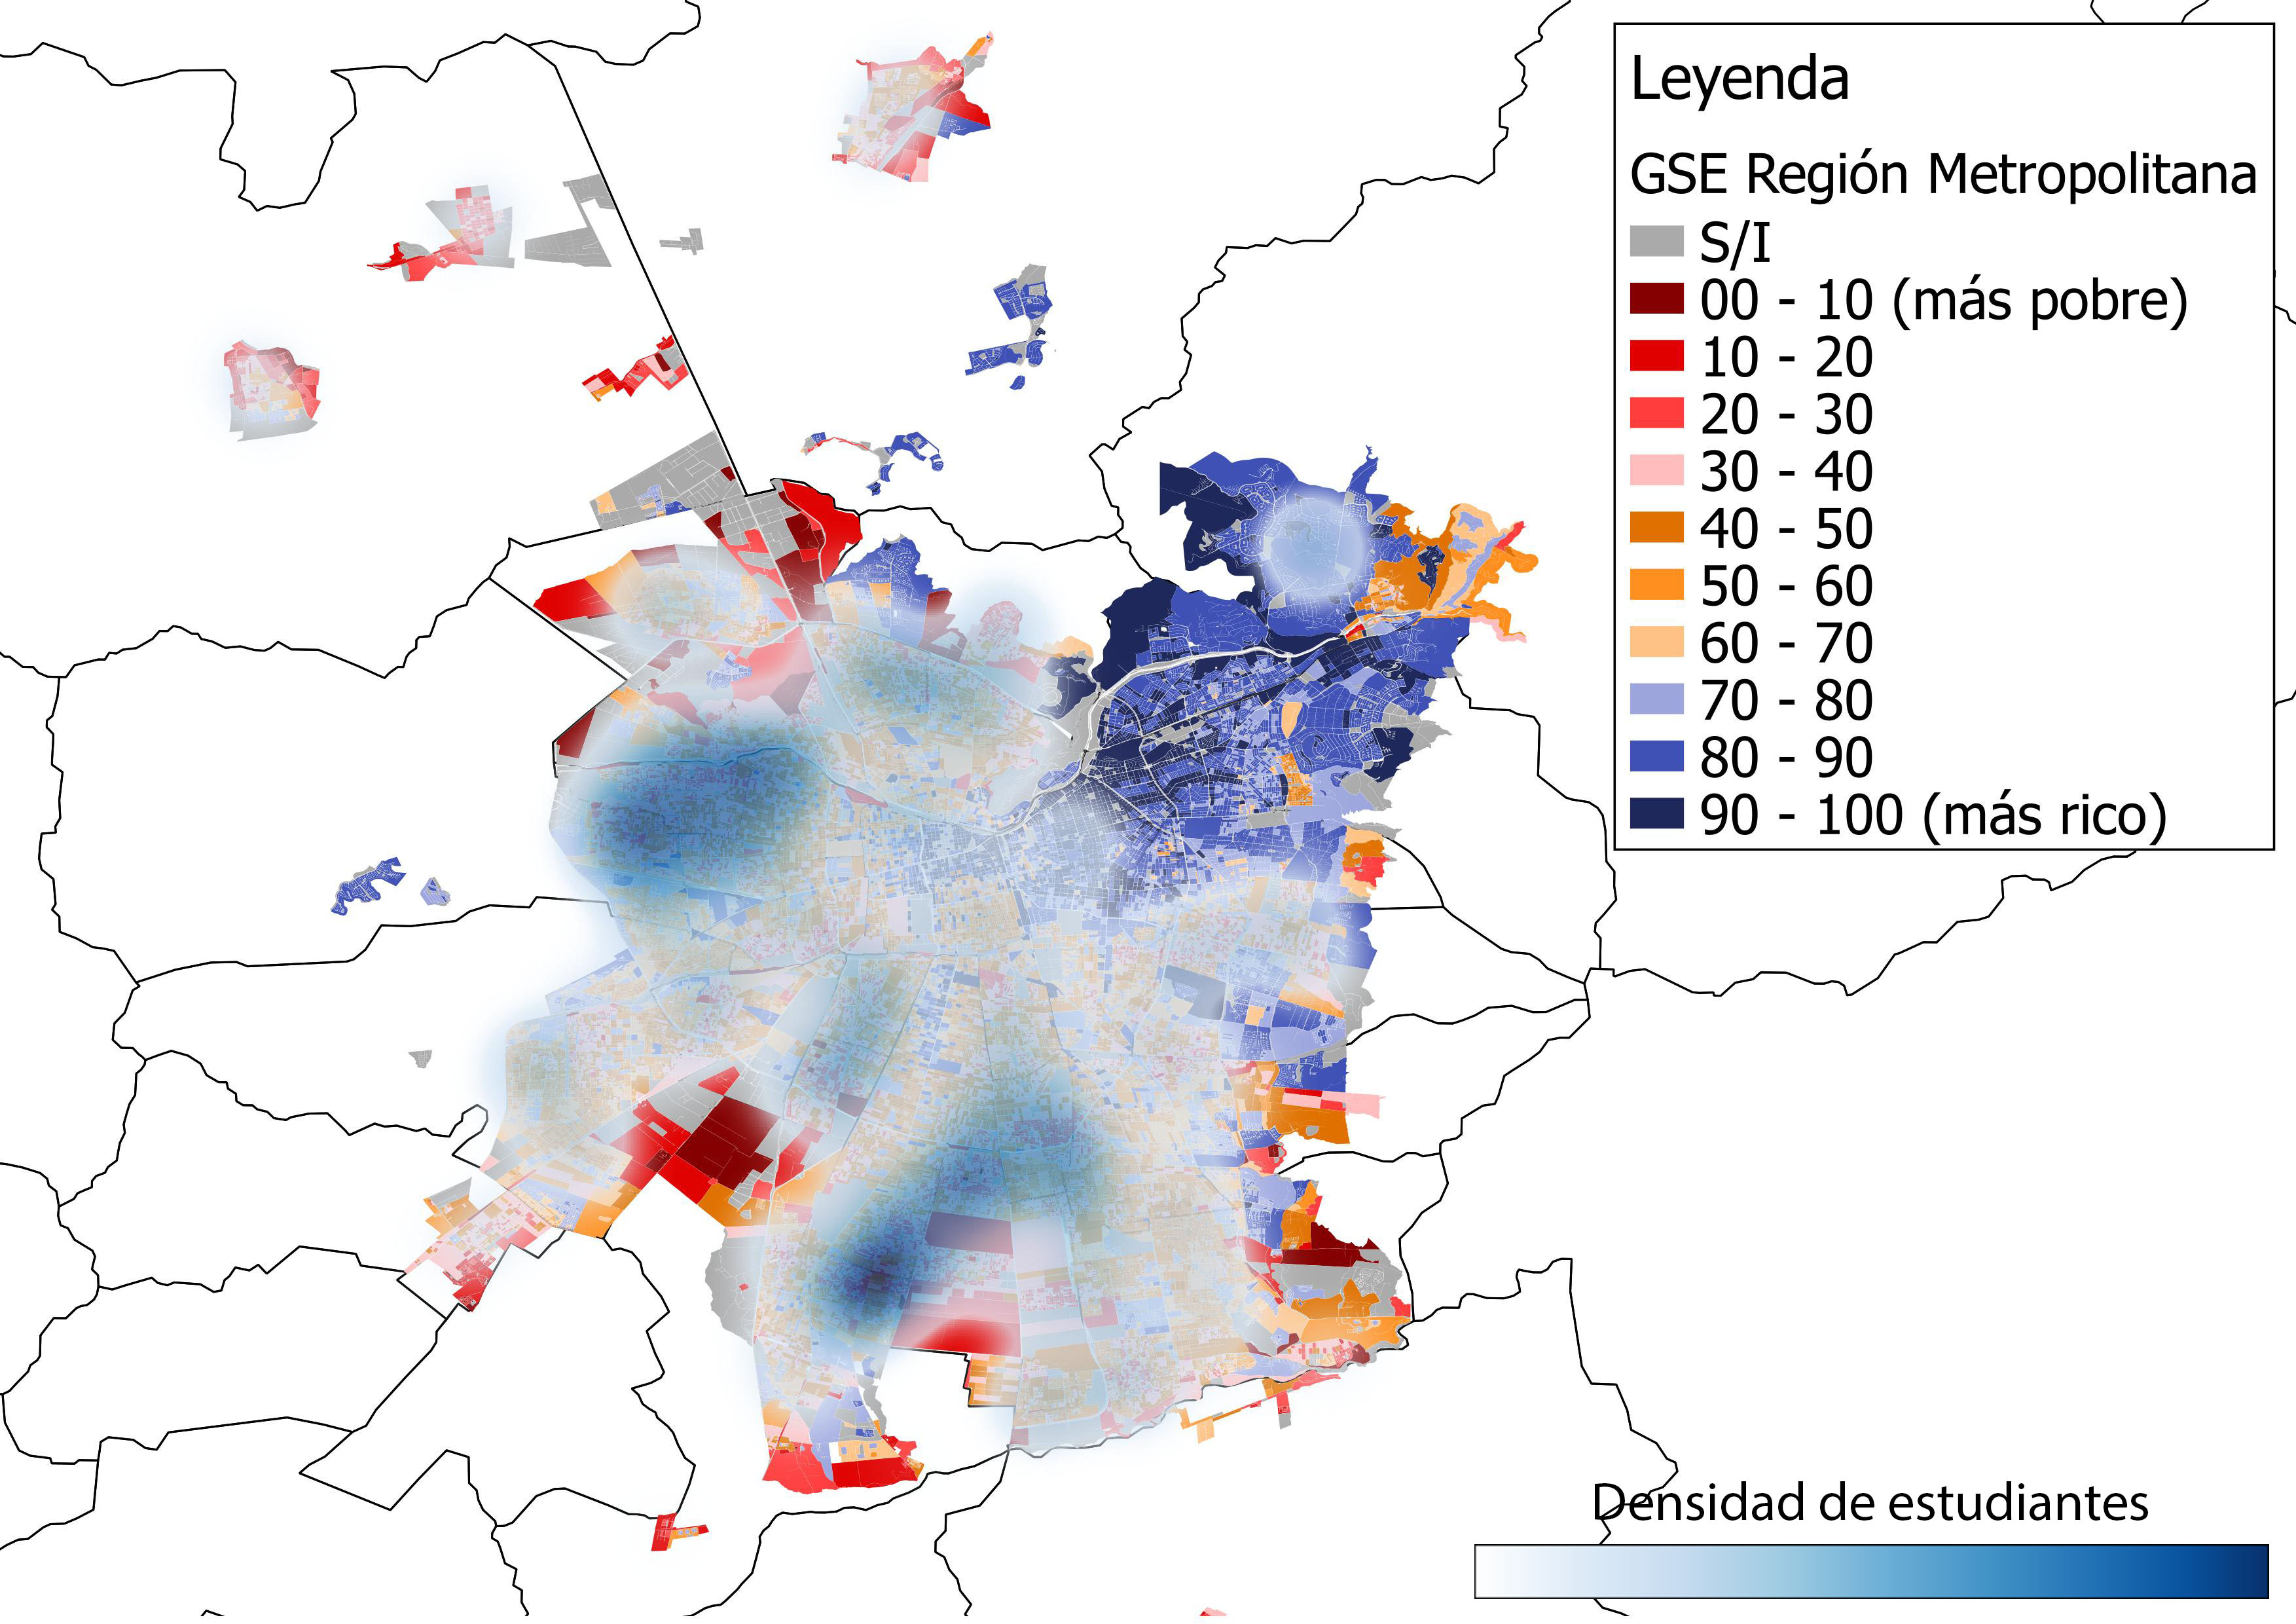
\includegraphics[width=7.5cm]{images/matriculas/E_CON_0_final.jpg}}
  \subfloat[Matrículas en colegios de E\_TODOS\_CON\_1.]{
   \label{f:}
    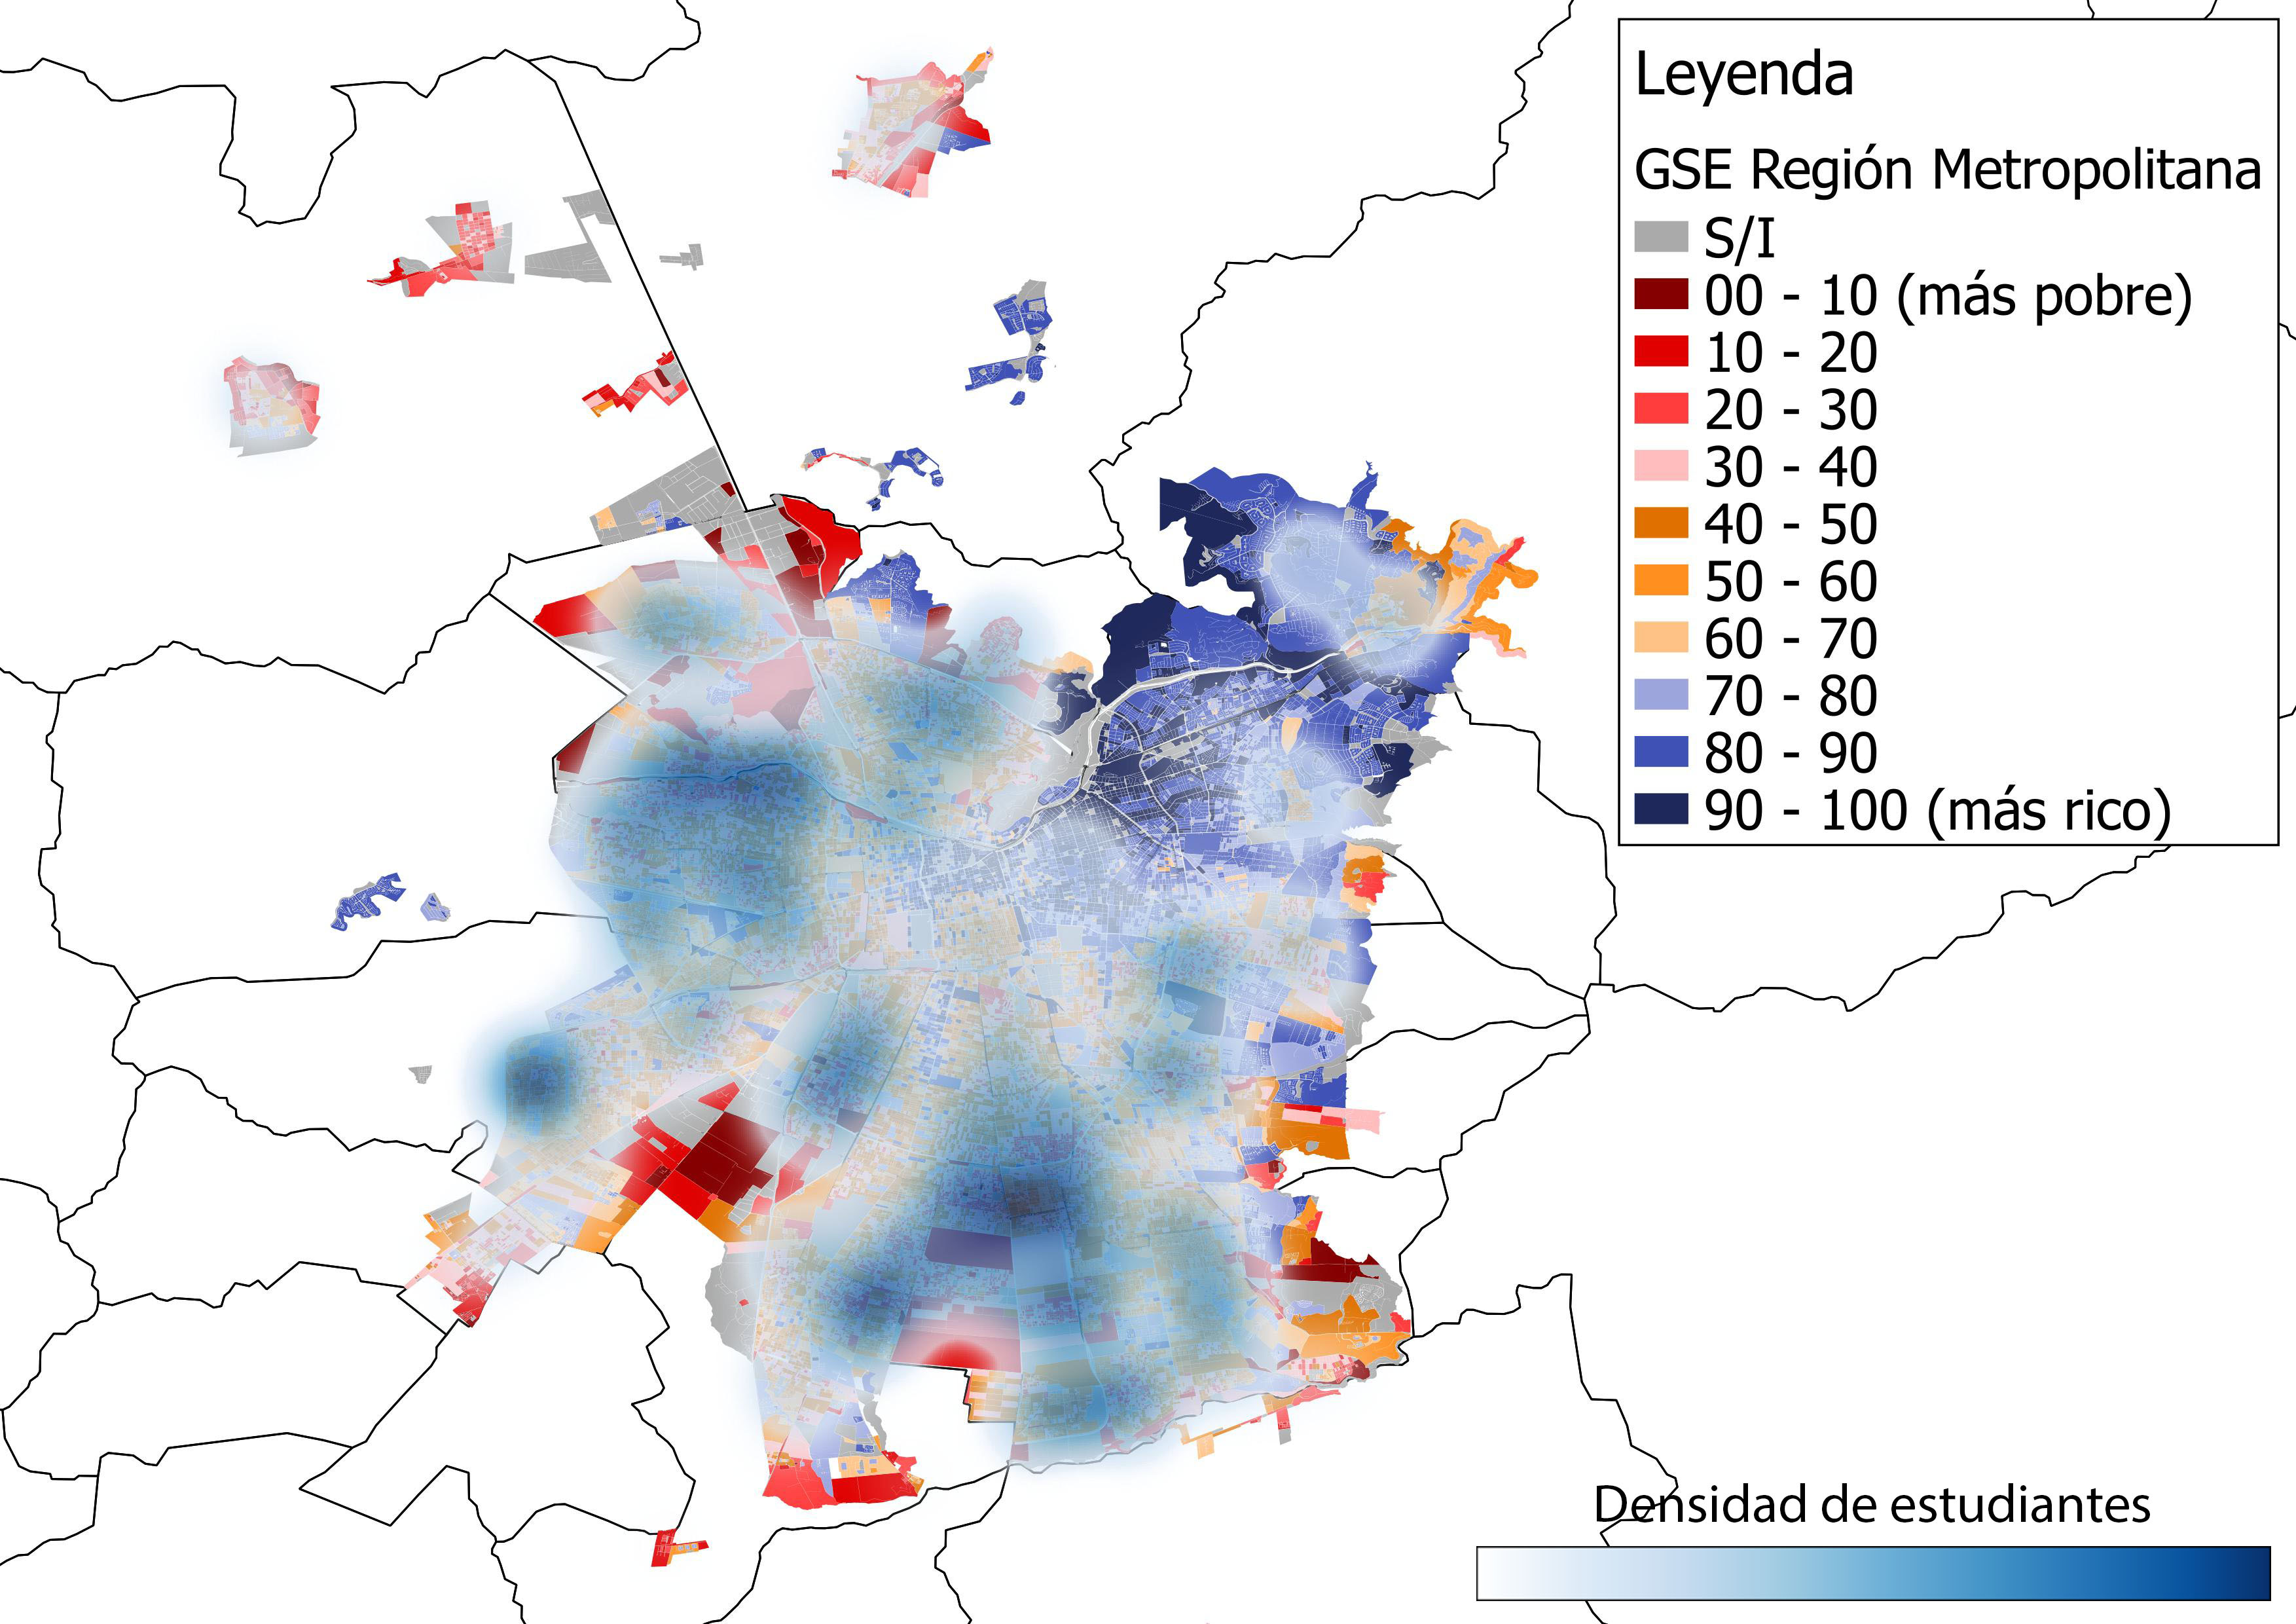
\includegraphics[width=7.5cm]{images/matriculas/E_CON_1_final.jpg}}\hspace{1mm}
  \subfloat[Matrículas en colegios de E\_TODOS\_CON\_2.]{
   \label{f:}
    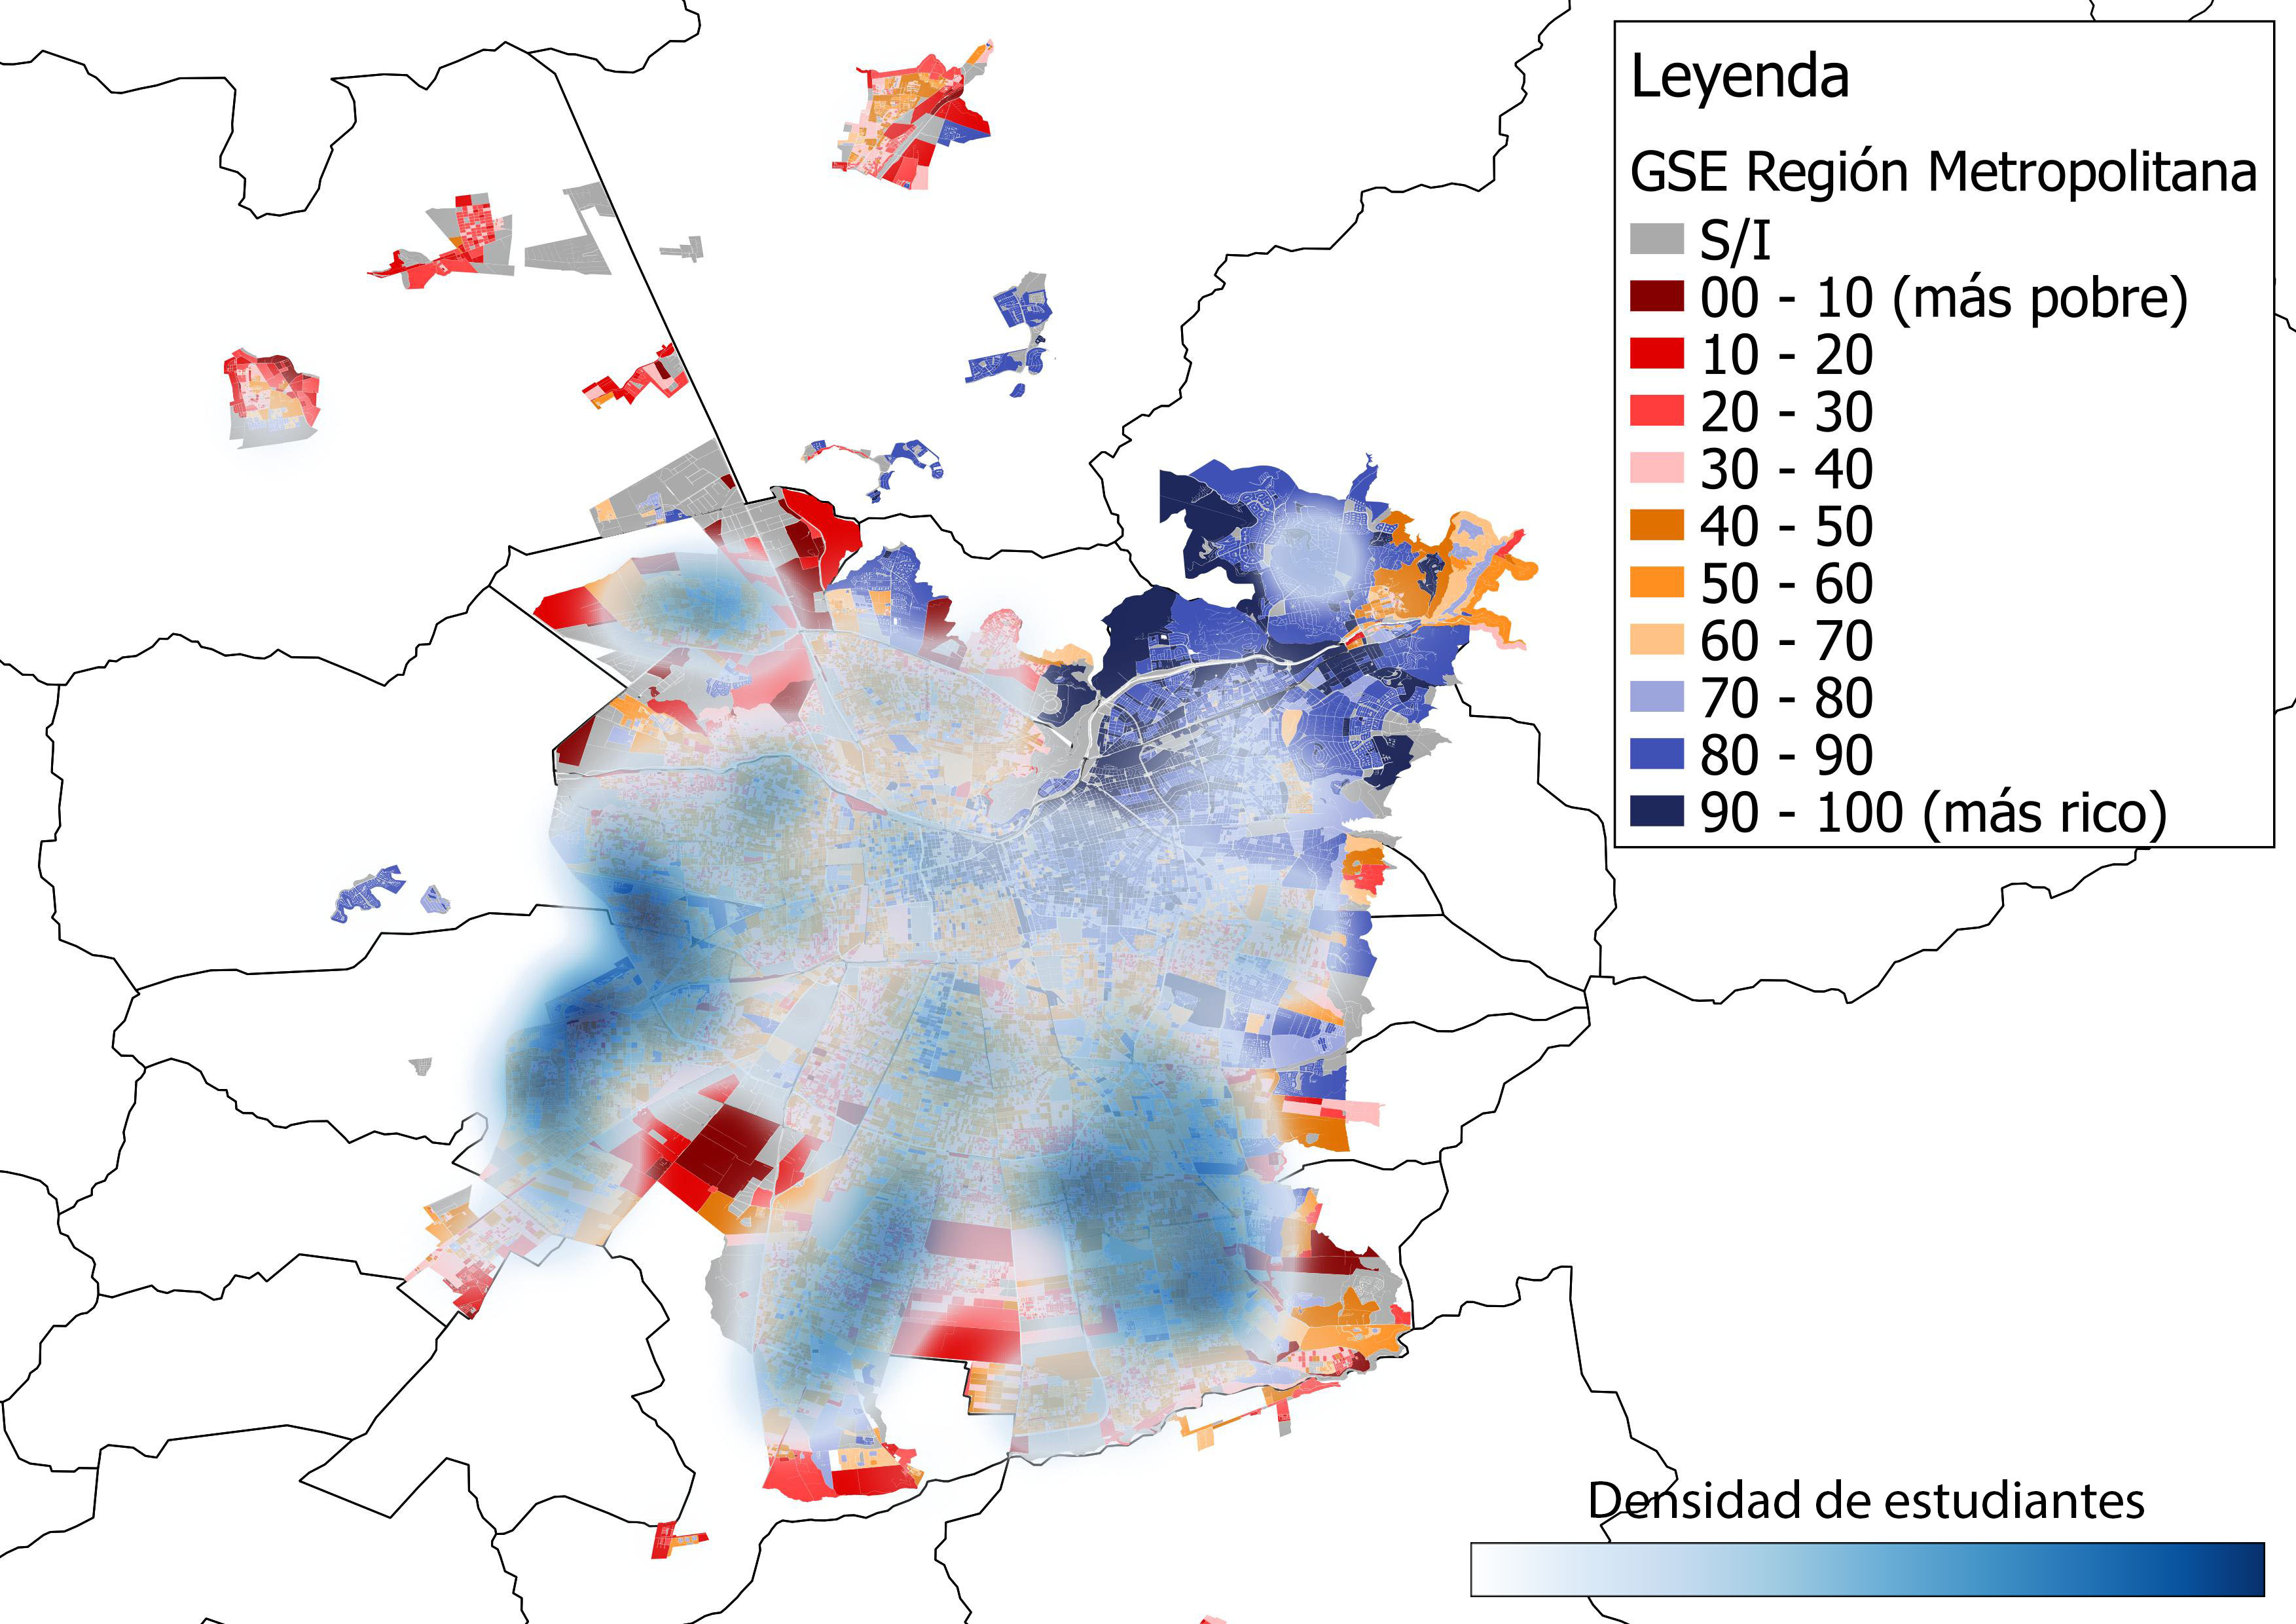
\includegraphics[width=7.5cm]{images/matriculas/E_CON_2_final.jpg}}
  \subfloat[Matrículas en colegios de E\_TODOS\_CON\_3.]{
   \label{f:}
    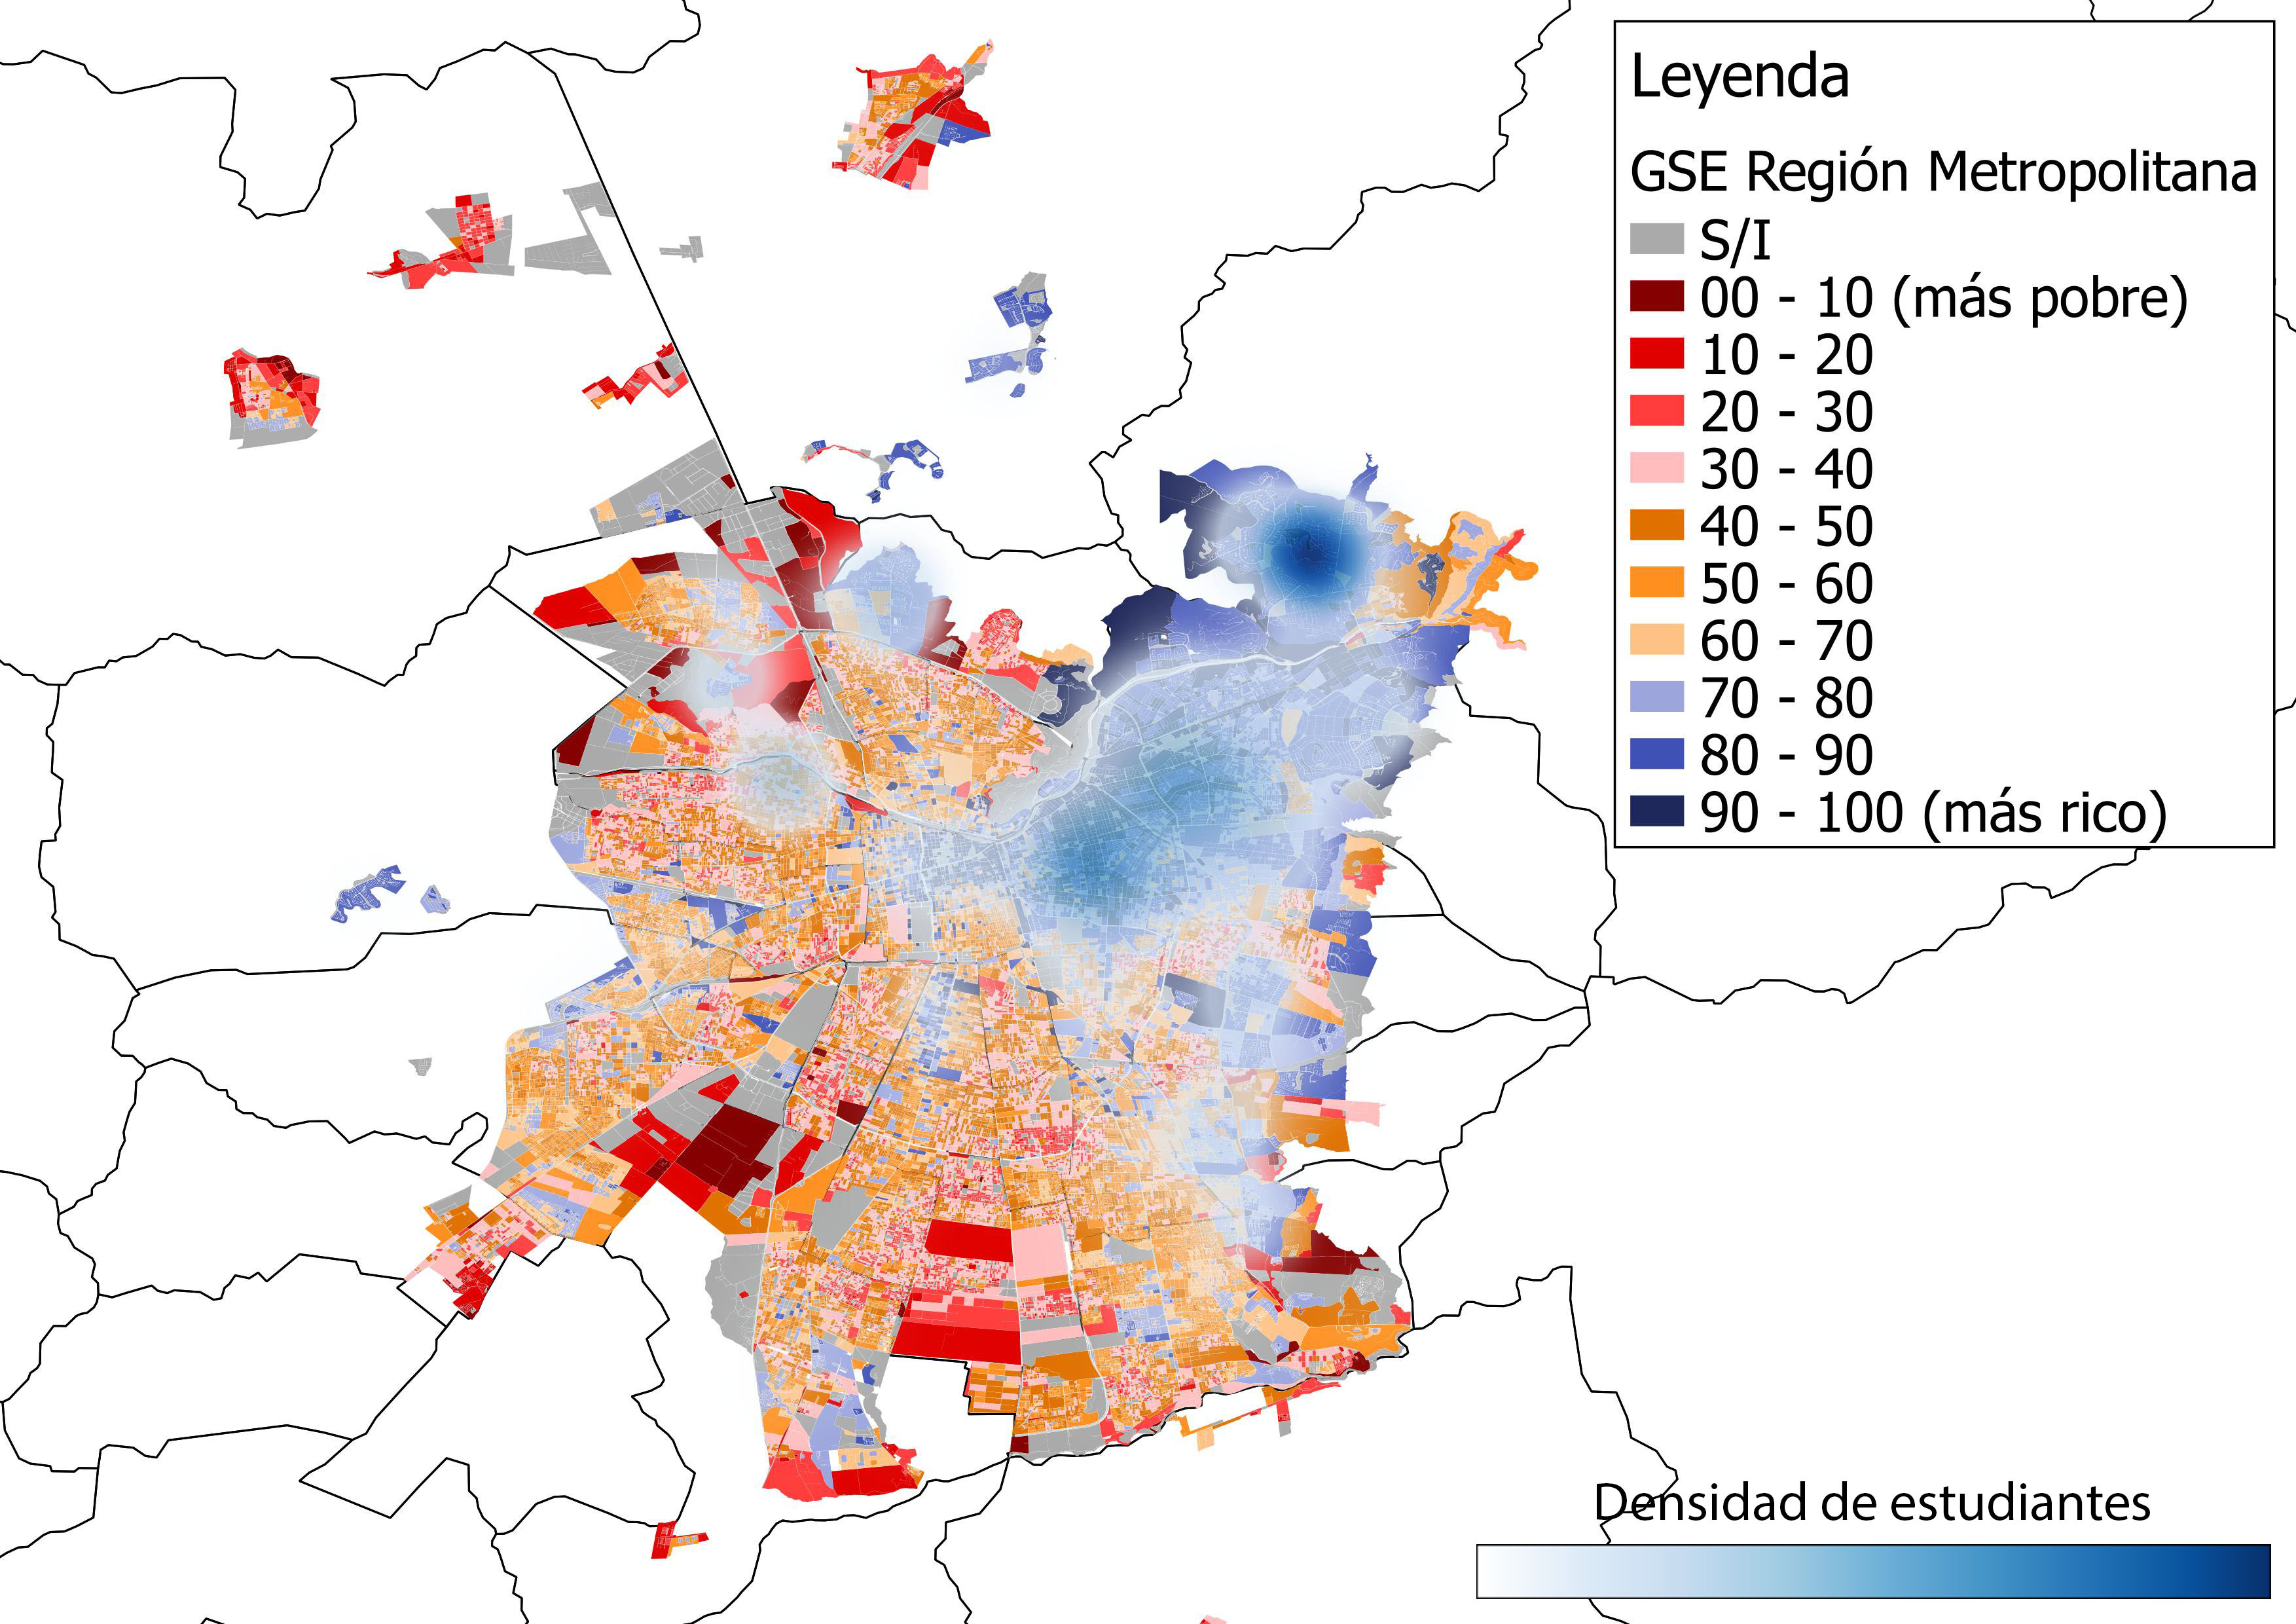
\includegraphics[width=7.5cm]{images/matriculas/E_CON_3_final.jpg}}
 \caption{Mapas de calor de matrículas (con atributos relacionales) en clústers de establecimientos sobre mapa GSE de la Región Metropolitana.}
 \label{f:}
\end{figure}

\begin{figure}[H]
 \centering
  \subfloat[Matrículas clúster M\_TODAS\_CON\_0.]{
   \label{f:}
    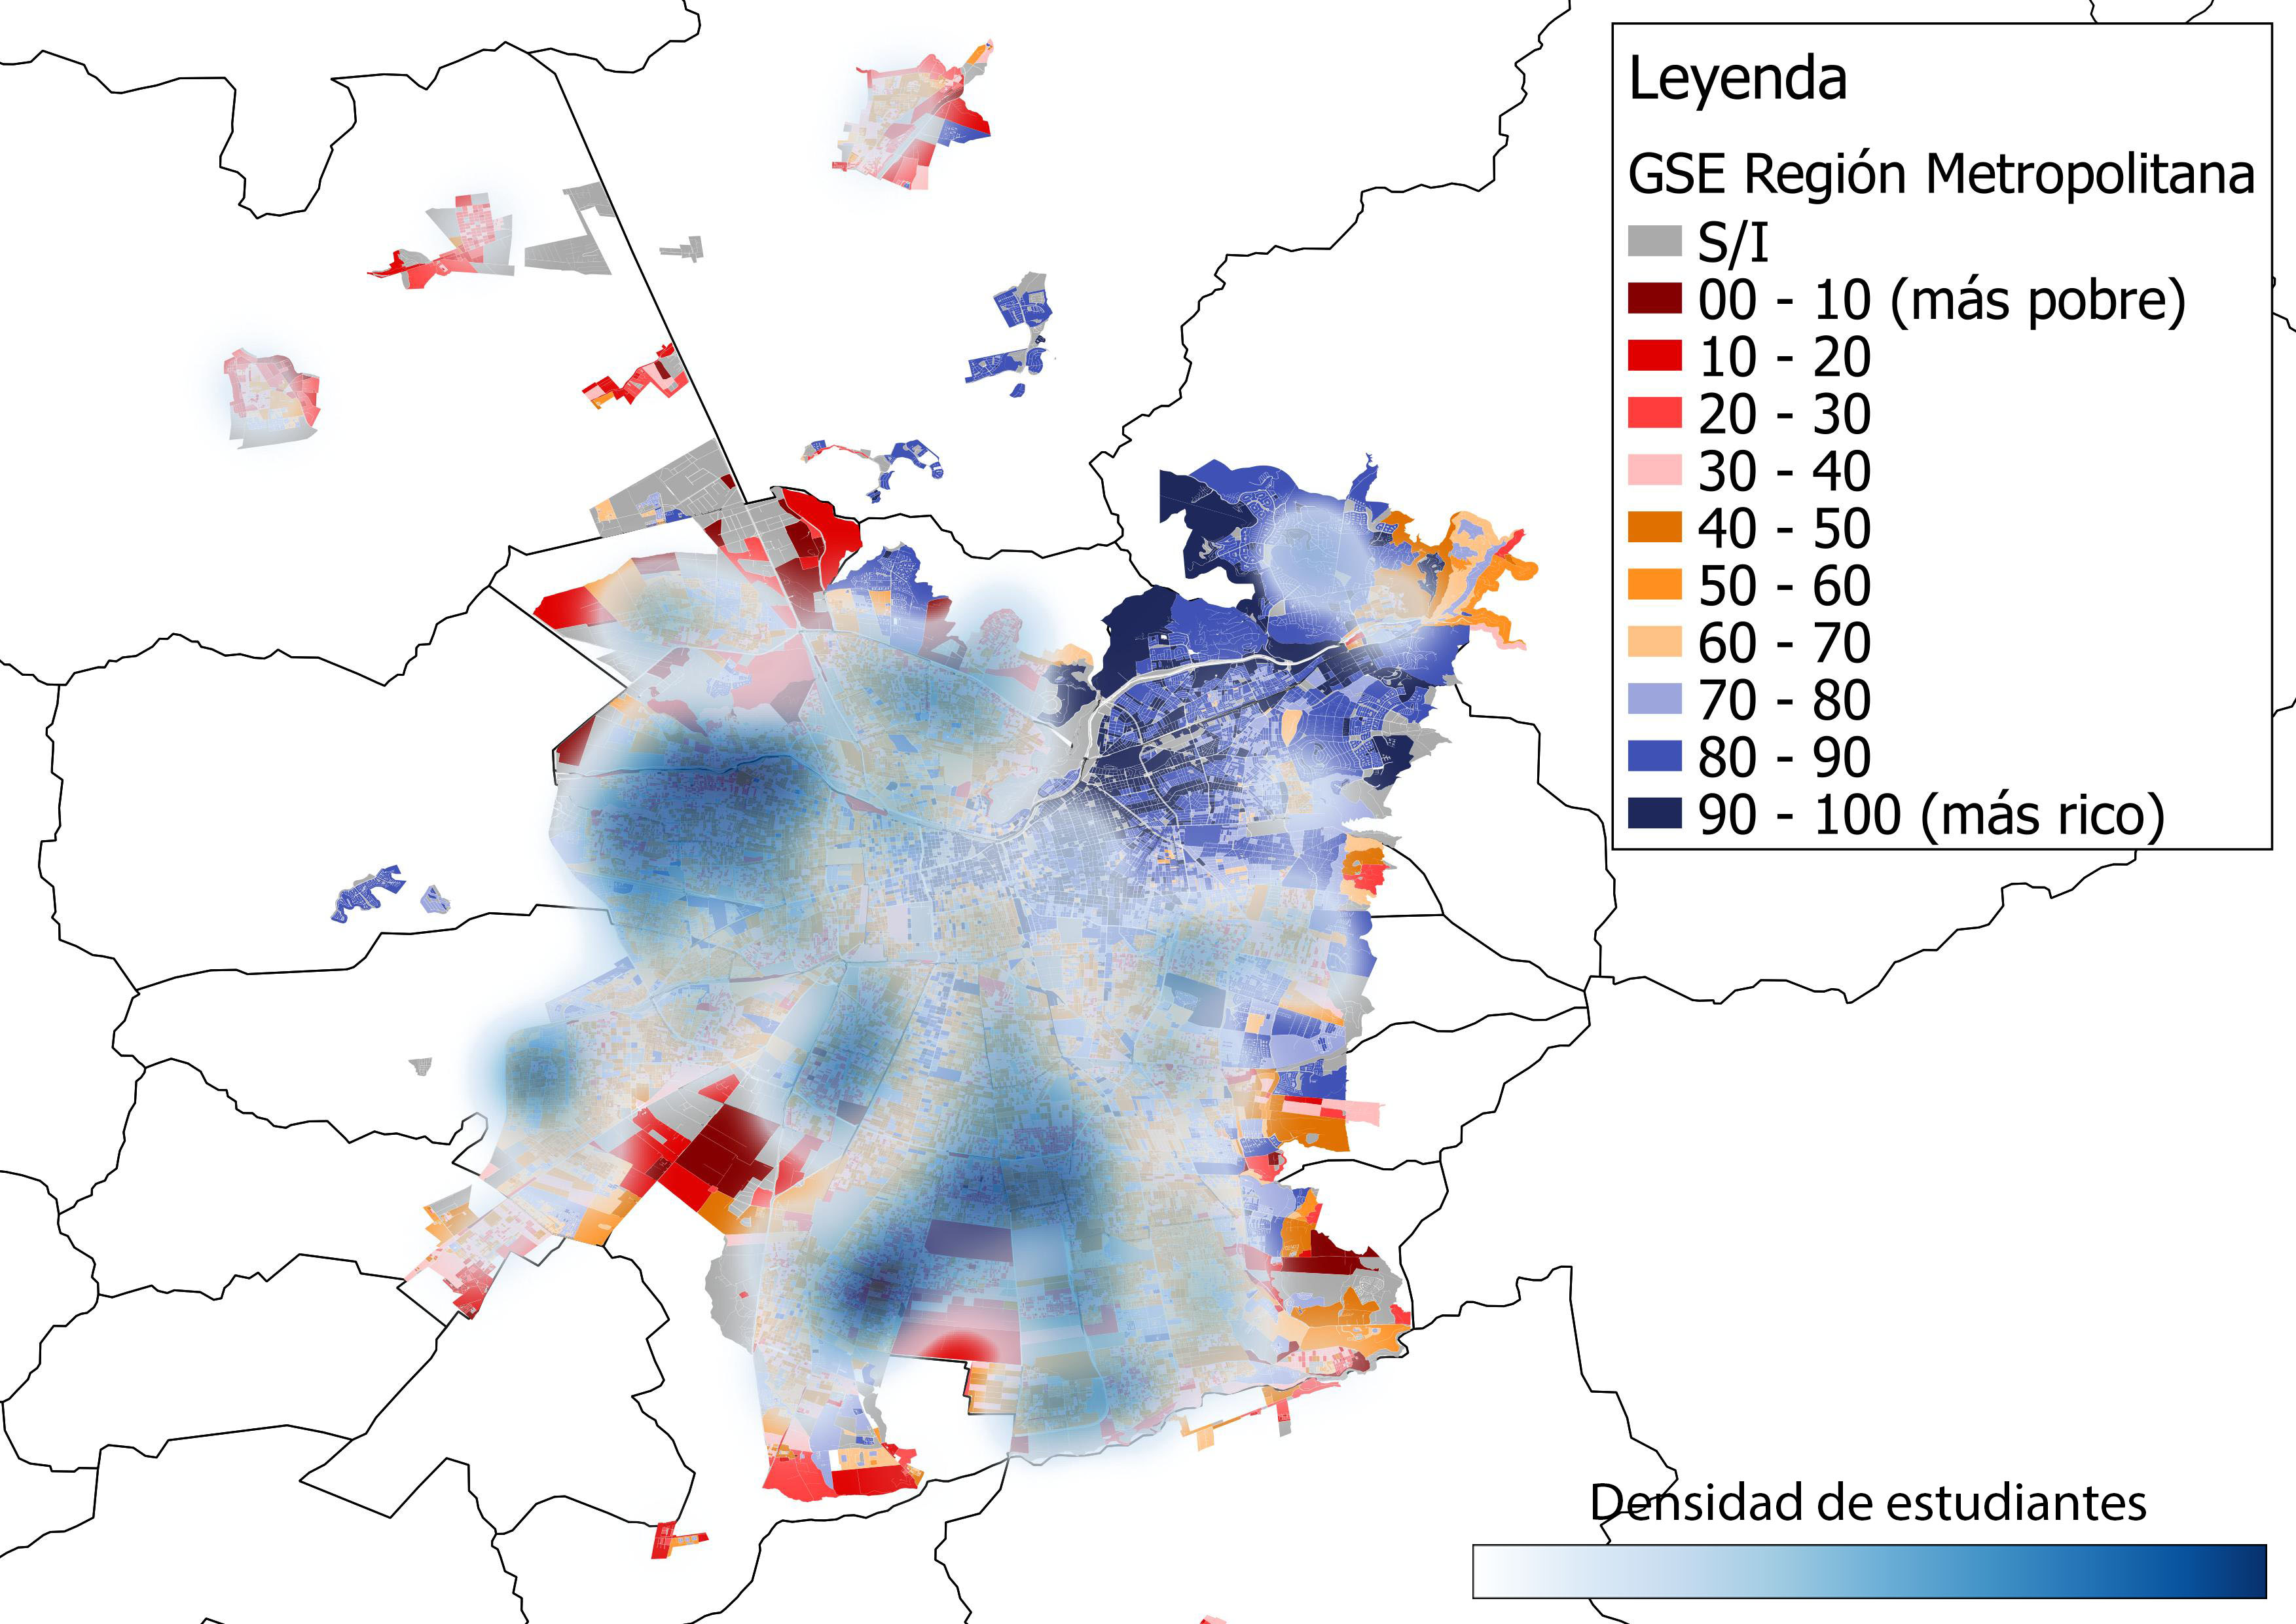
\includegraphics[width=7.5cm]{images/matriculas/M_CON_0_final.jpg}}
  \subfloat[Matrículas clúster M\_TODAS\_CON\_1.]{
   \label{f:}
    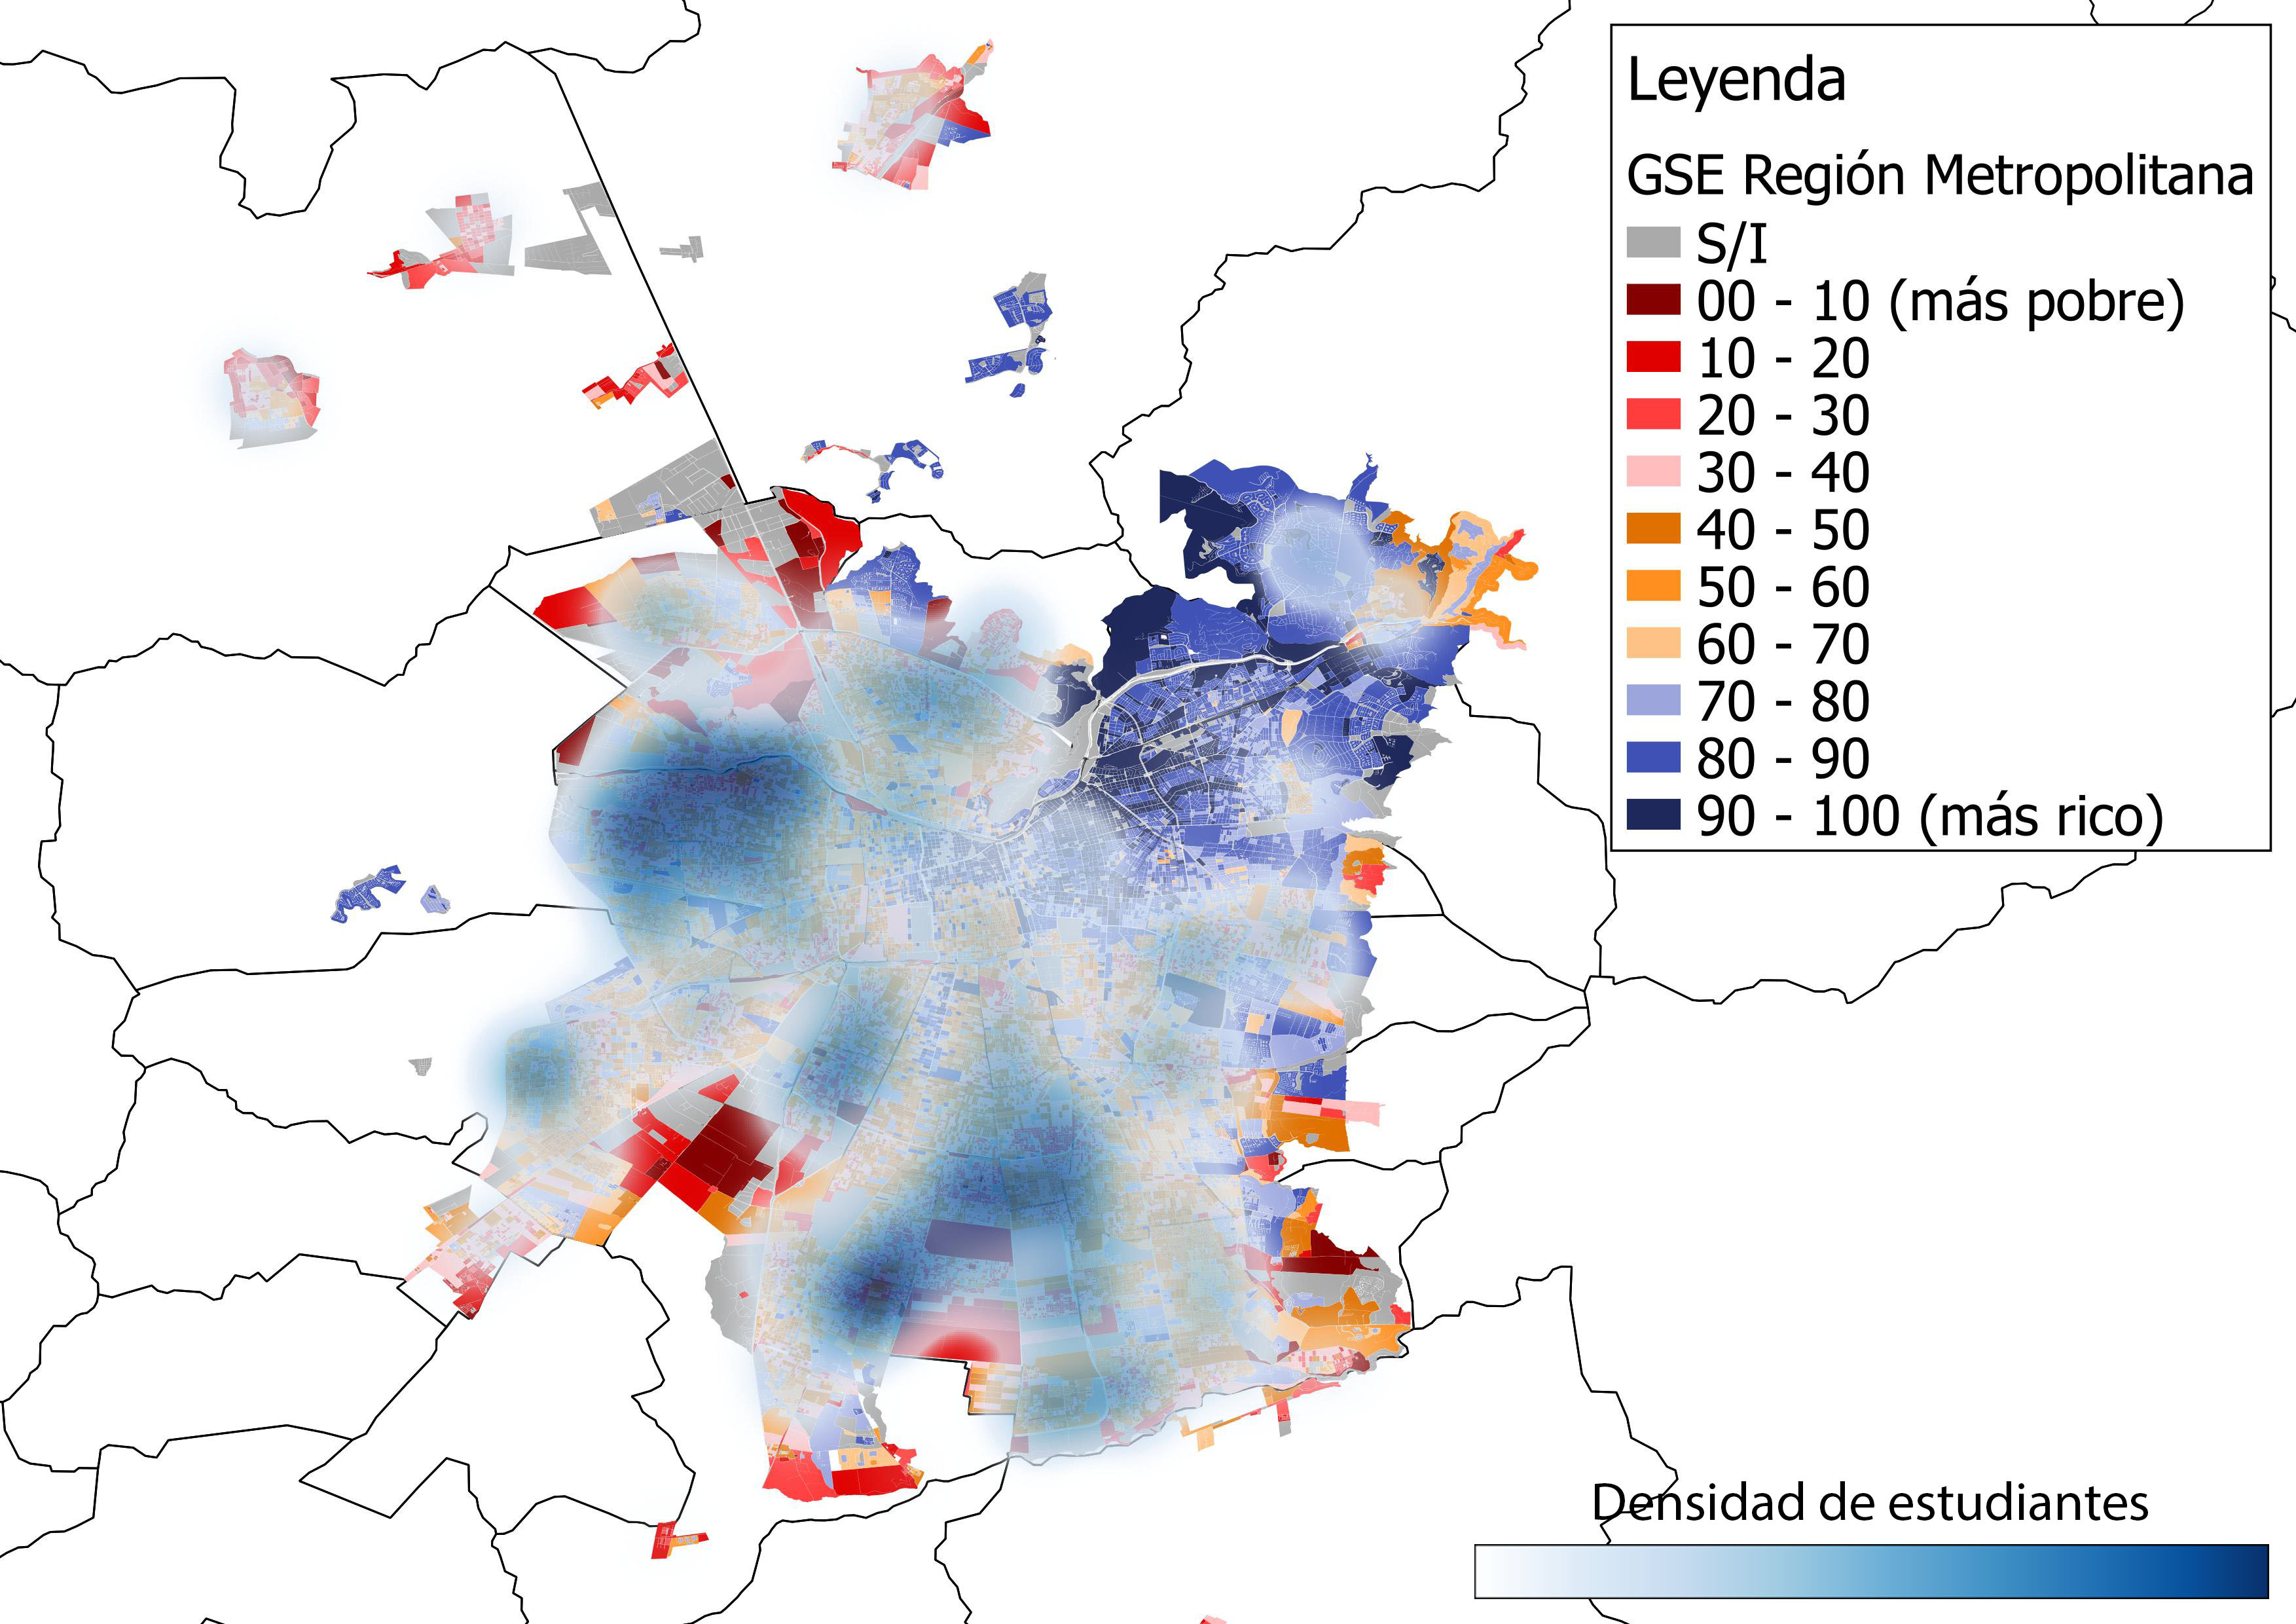
\includegraphics[width=7.5cm]{images/matriculas/M_CON_1_final.jpg}}\hspace{1mm}
  \subfloat[Matrículas clúster M\_TODAS\_CON\_2.]{
   \label{f:}
    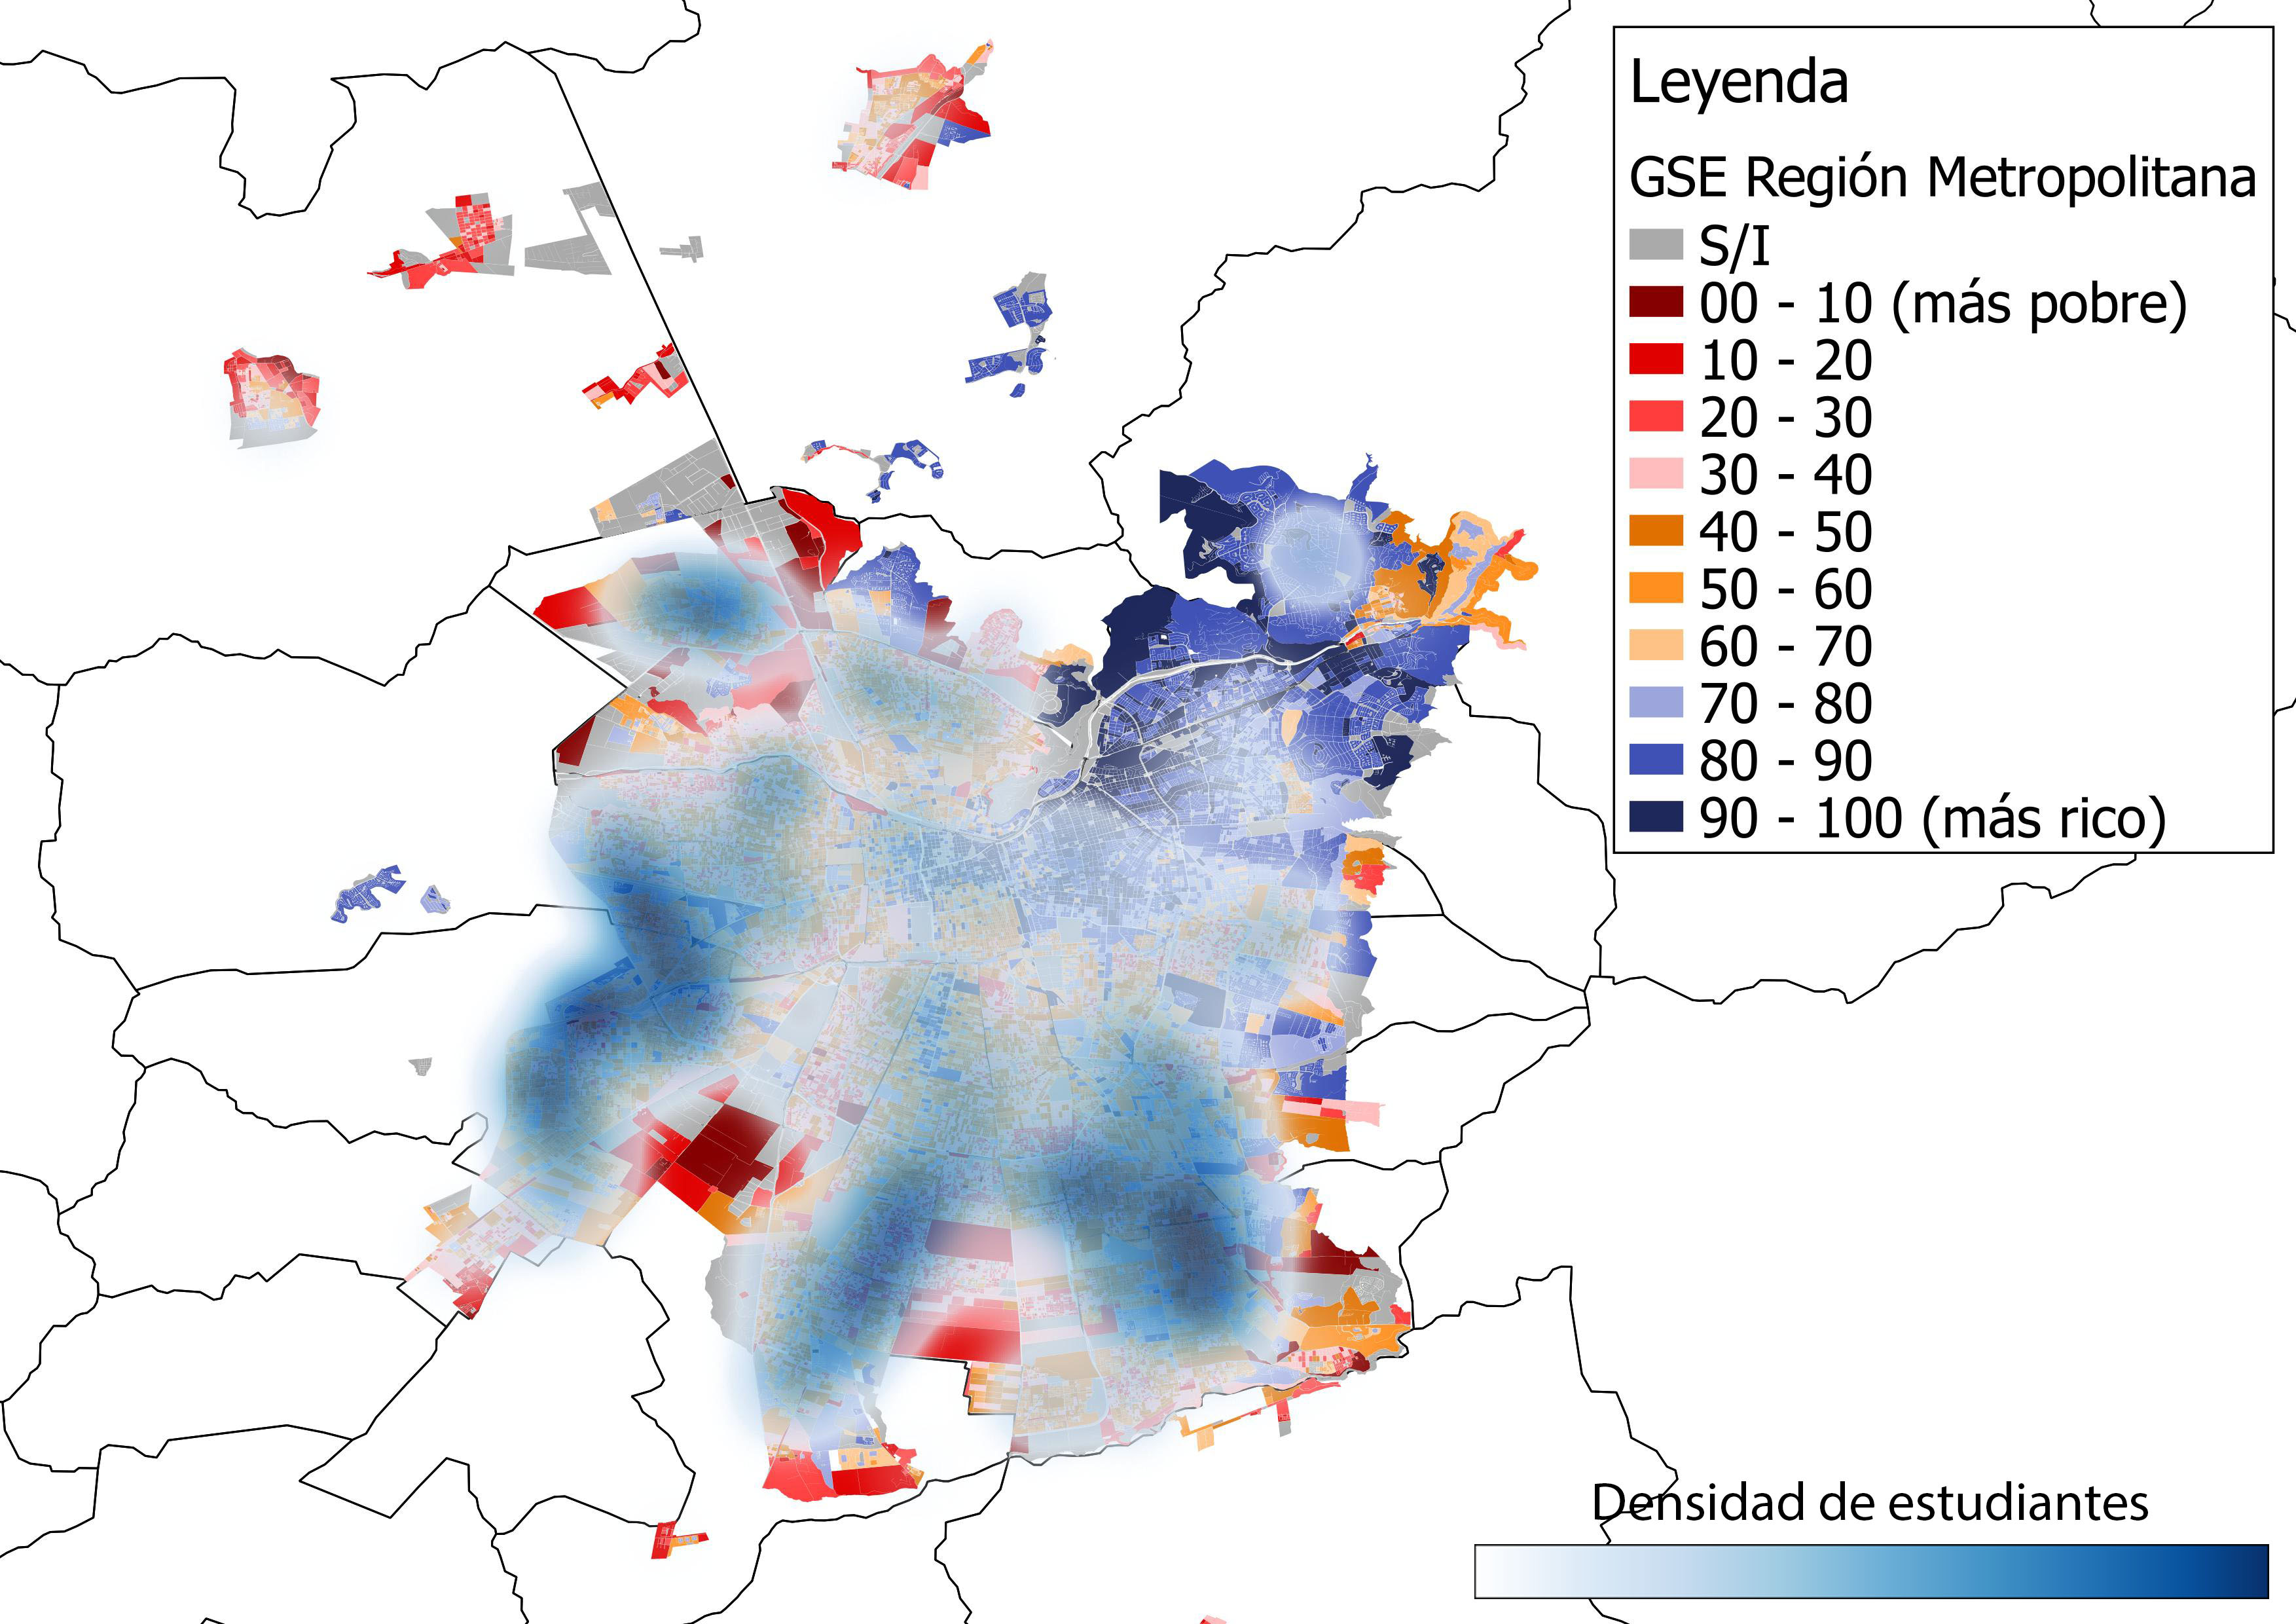
\includegraphics[width=7.5cm]{images/matriculas/M_CON_2_final.jpg}}
  \subfloat[Matrículas clúster M\_TODAS\_CON\_3.]{
   \label{f:}
    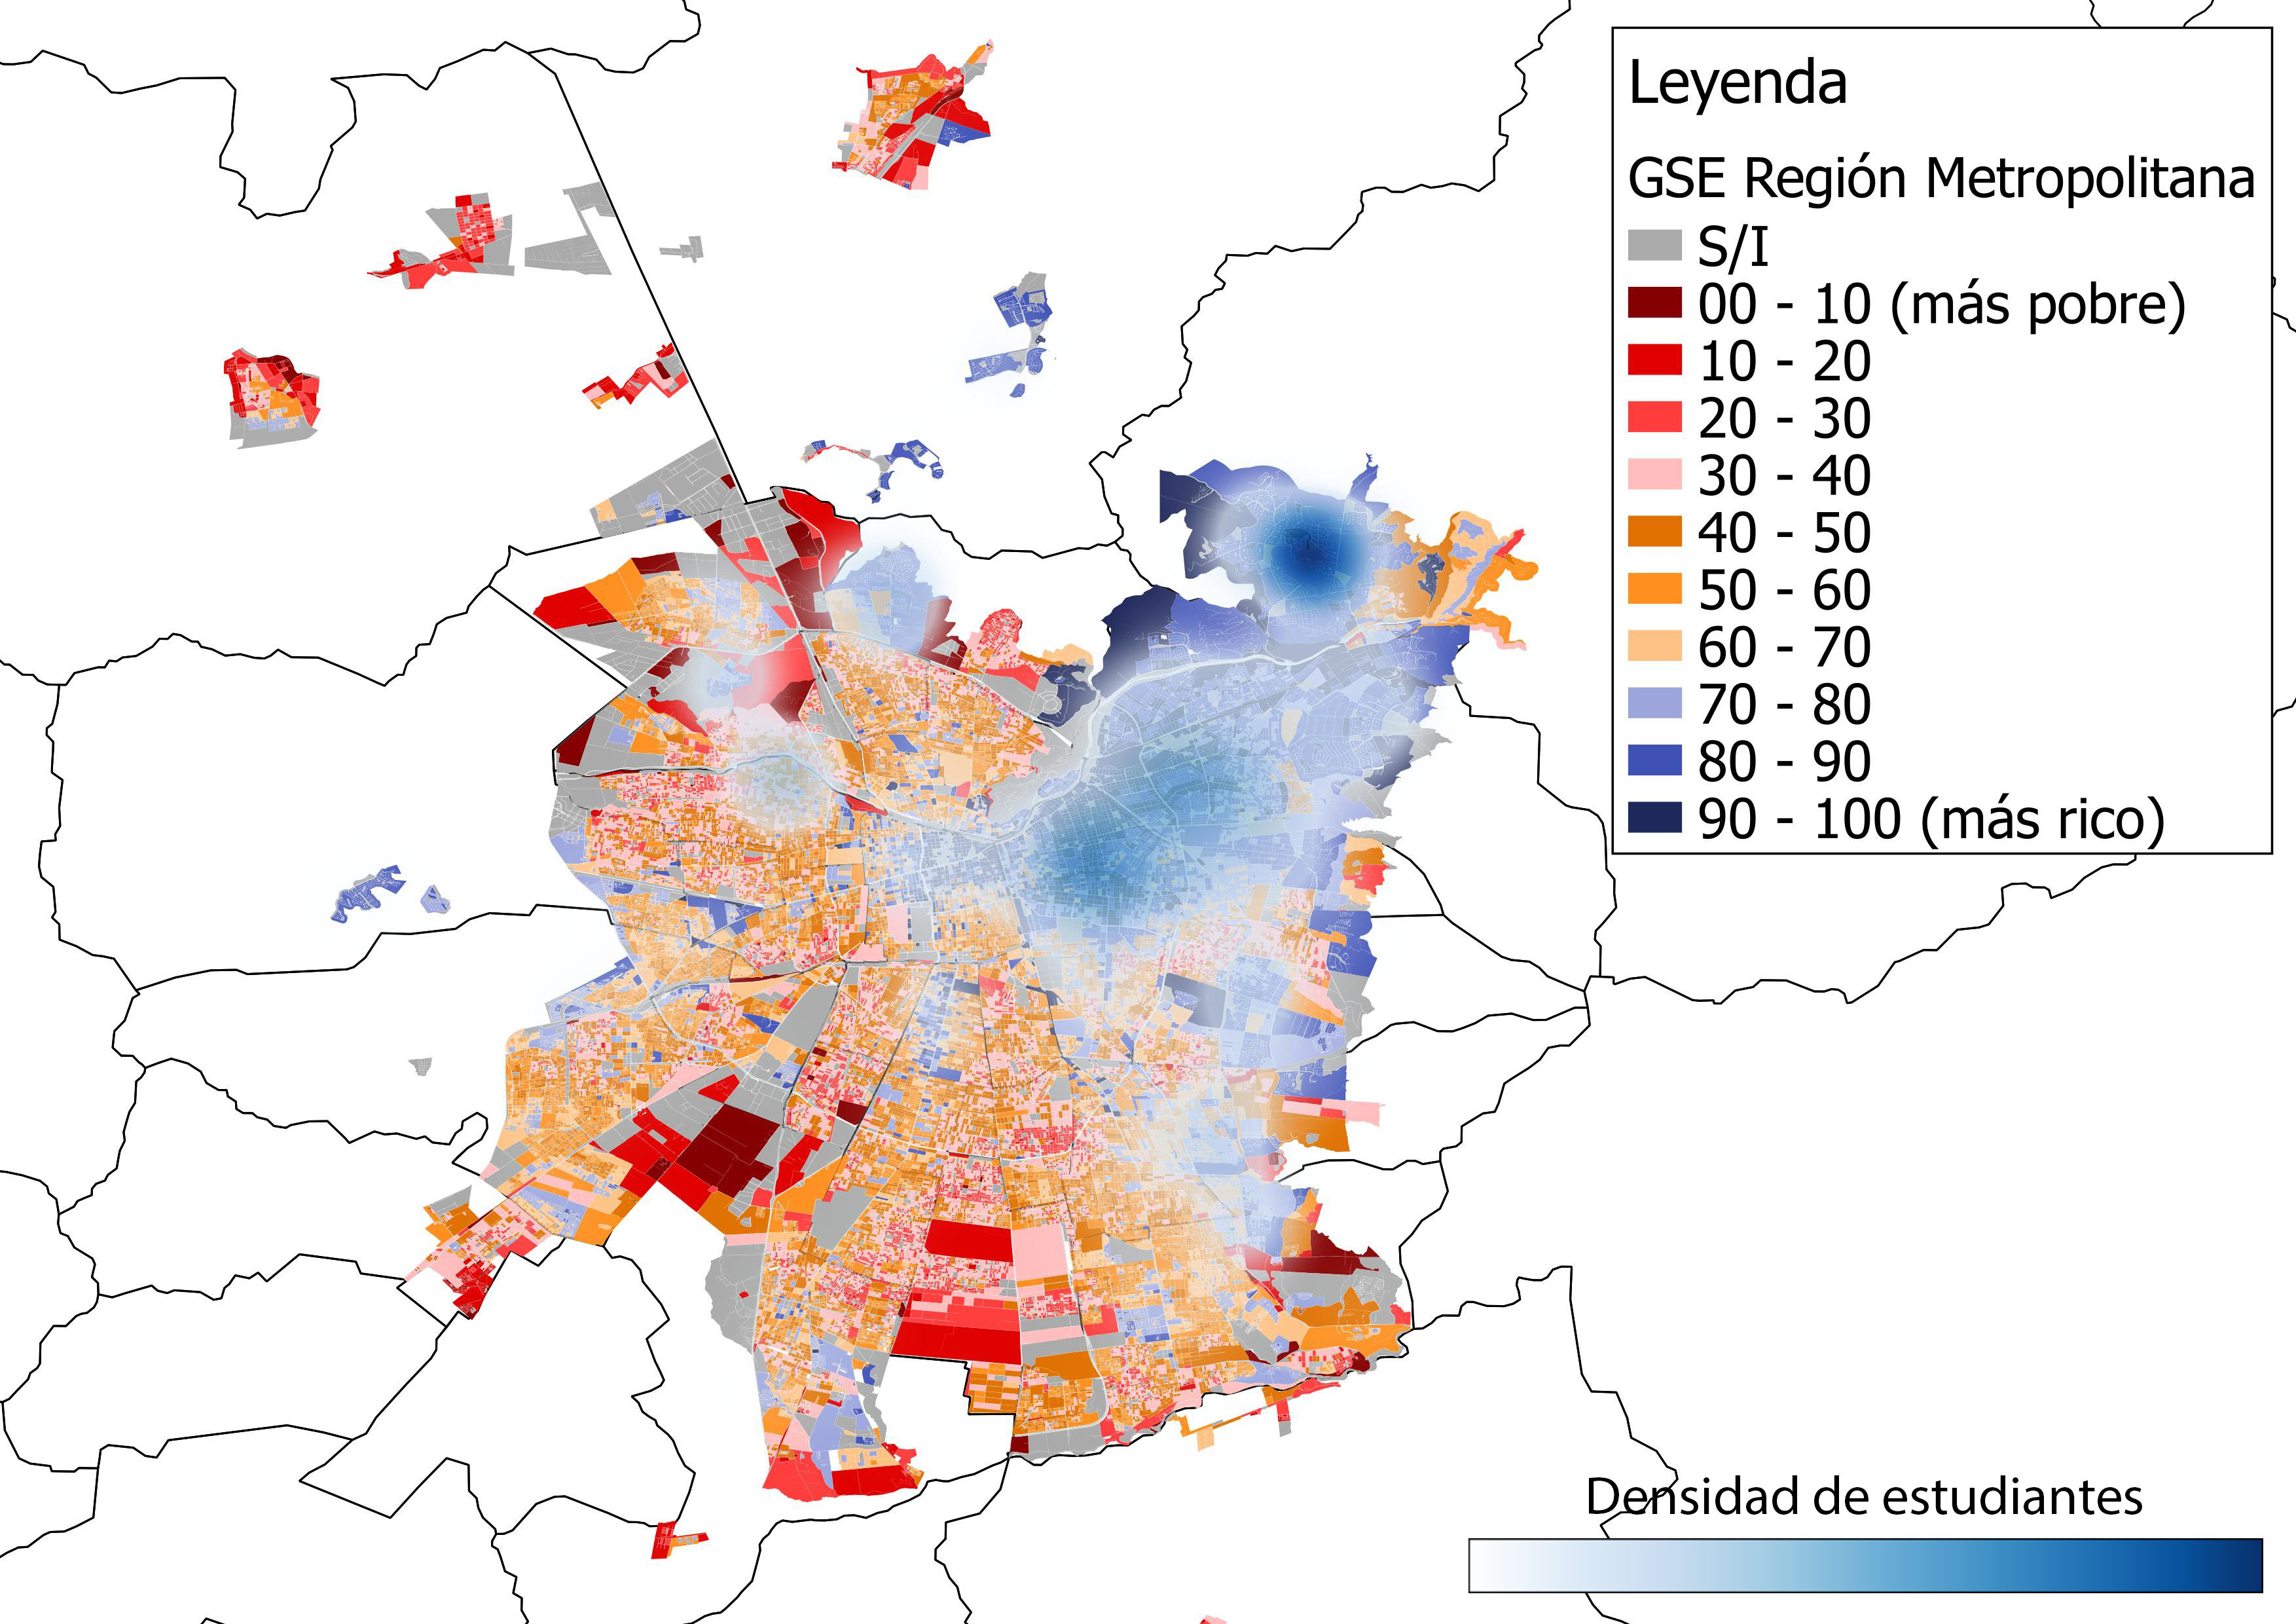
\includegraphics[width=7.5cm]{images/matriculas/M_CON_3_final.jpg}}
 \caption{Mapas de calor de clústers de matrículas (con atributos relacionales) sobre mapa GSE de la Región Metropolitana.}
 \label{f:}
\end{figure}